\documentclass[sigconf, anonymous]{acmart}

\fancyhf{} % Remove fancy page headers 
\fancyhead[C]{Anonymous submission \#9999 to ACM CCS 2017} % TODO: replace 9999 with your paper number
\fancyfoot[C]{\thepage}

\setcopyright{none} % No copyright notice required for submissions
\acmConference[Anonymous Submission to ACM CCS 2017]{ACM Conference on Computer and Communications Security}{Due 19 May 2017}{Dallas, Texas}
\acmYear{2017}

\settopmatter{printacmref=false, printccs=true, printfolios=true} % We want page numbers on submissions

%%\ccsPaper{9999} % TODO: replace with your paper number once obtained

%packages
\usepackage{natbib}
\usepackage{amsmath}
\usepackage{amsthm}
\usepackage{mathtools}
\usepackage{mdframed}
\usepackage{subfigure}
\usepackage{booktabs}
% \usepackage{hyperref}
\usepackage{subfigure}
\usepackage{siunitx} % Provides the \SI{}{} and \si{} command for typesetting SI units
\usepackage{graphicx} % Required for the inclusion of images
% \usepackage{natbib} % Required to change bibliography style to APA
\usepackage{datetime}
\usepackage{lscape}
\usepackage{algorithm}
\usepackage{algorithmic}
\usepackage{xspace}
\usepackage[english]{babel} % English language/hyphenation
\usepackage{proof}
\usepackage{booktabs} % Top and bottom rules for tables
\usepackage[colorlinks, allcolors = blue,]{hyperref}
\usepackage{accents}
\usepackage{amsfonts}
\usepackage{stmaryrd}
\usepackage{amsmath,amsthm,amssymb,latexsym} 
\usepackage{microtype}
\usepackage{graphicx}
\usepackage{subfigure}
\usepackage{booktabs} % for professional tables
\usepackage{hyperref}
\usepackage{icml2019}
\usepackage{lipsum}

\usepackage{authblk}


%new commands
\newcommand{\theHalgorithm}{\arabic{algorithm}}
\newtheorem{definition}{Definition}
\usepackage{cancel}
\usepackage[normalem]{ulem}
\newcommand{\dataobs}{\textbf{x}}
\newcommand{\adj}[2]{\textbf{adj}(#1,#2)}
\newcommand{\candidateset}{\mathcal{R}_{\textup{post}}}
\newcommand{\bprior}{\boldsymbol{\beta}_{\textup{prior}}}
\newcommand{\bysinfer}{\mathsf{Infer}}
\newcommand{\betad}{\mathsf{Beta}}
\newcommand{\betaf}{\textup{B}}
\newcommand{\mbetaf}{\boldsymbol{\textup{B}}}
\newcommand{\vtheta}{\boldsymbol{\theta}}
\newcommand{\valpha}{\boldsymbol{\alpha}}
\newcommand{\vbeta}{\boldsymbol{\beta}}
\newcommand{\lapmech}{\mathsf{LSDim}}
\newcommand{\ilapmech}{\mathsf{LSHist}}
\newcommand{\binomial}[2]{\mathsf{Bin}(#1, #2)}
\newcommand{\multinomial}[2]{\mathsf{Mult}(#1, #2)}
\newcommand{\expmech}{\mathsf{EHD}}
\newcommand{\hexpmech}{\mathsf{EHDS}}
\newcommand{\lexpmech}{\mathsf{EHDL}}
\newcommand{\hexpmechd}{\mathsf{expMech}^{D}_{\hellinger}}
\newcommand{\privinfer}{\mathsf{PrivInfer}}
\newcommand{\hlg}{\mathsf{H}}
\newcommand{\dirichlet}[1]{\mathsf{Dir}(#1)}
\newcommand{\alphas}{\boldsymbol{\alpha}}
\newcommand{\xis}{\boldsymbol{\xi}}
\newcommand{\iverson}[1]{[#1]}
\newcommand{\datauni}{\mathcal{X}}
\newcommand{\hellinger}{\mathcal{H}}
\newcommand{\ux}[1]{u(\textbf{x}, {#1})}
\newcommand{\uxadj}[1]{u(\textbf{x}', {#1})}
\newcommand{\cardinality}[2]{\mathcal{C}^{#1}_{#2}}
\newcommand{\range}{\mathcal{O}}
\newcommand{\nomalizer}[1]{\sum\limits_{r'\in \mathcal{R}_{\textup{post}}} \exp \big(\frac{-\epsilon\cdot \mathcal{H} (\mathsf{BI}(#1),r')}{4 \cdot S(#1)}\big)}

\newcommand{\unomalizer}[1]{\sum\limits_{r'\in \mathcal{R}_{\textup{post}}} \exp \big(\frac{-\epsilon\cdot u(#1, r')}{4 \cdot S(#1)}\big)}


\newcommand{\hexpmechPr}[2]{\underset{z \thicksim \hexpmech(#1)}{\Pr}\left[ #2 \right]}
\newcommand{\lapmechPr}[2]{\underset{z \thicksim \lapmech(#1)}{\Pr}\left[ #2 \right]}

\newcommand{\ilapmechPr}[2]{\underset{
{z \thicksim \ilapmech(#1)}
}{\Pr}\left[ #2 \right]}

\newtheorem{thm}{Theorem}[section]

\newtheorem{lem}{Lemma}[section]

\newtheorem{assert}{Assertion}[lem]
\newcommand{\lap}[2]{\mathsf{Lap}(#1, #2)}
\newcommand{\todo}[1]{{\footnotesize \color{red}\textbf{[[ #1 ]]}}}

\begin{document}
\title{Sketch of DP - Bayesian Inference} % TODO: replace with your title

\begin{abstract}
  Bayesian inference is a statistical method which allows to derive a
\emph{posterior} distribution over a parameter, starting from a
\emph{prior} distribution and observed data.  Many works have focused
on making this process differentially private adding noise on the
parameters representing the distributions\todo{cite?}.  Also, the
accuracy was measured using metrics on  the numeric
parameters representing the posterior distribution, e.g. $\ell_1$-norm
\todo{cite?}.
  
In this work we present a new mechanism for differentially private Bayesian
inference where the noise is calibrated w.r.t  a smooth
sensitivity computed with a metric on probability distributions.
We also measure the accuracy of the process by using a metric over
probability measures.  We compared the accuracy of this approach with
the one based on the $\ell_1$-norm.  We present experimental results
showing that the former outperforms the latter.

\end{abstract}


% TODO: replace this section with code generated by the tool at https://dl.acm.org/ccs.cfm
\begin{CCSXML}
<ccs2012>
<concept>
<concept_id>10002978.10003029.10011703</concept_id>
<concept_desc>Security and privacy~Usability in security and privacy</concept_desc>
<concept_significance>500</concept_significance>
</concept>
</ccs2012>
\end{CCSXML}

\ccsdesc{Security and privacy~Use https://dl.acm.org/ccs.cfm to generate actual concepts section for your paper}
% -- end of section to replace with generated code

\keywords{differential privacy, Bayesian inference, Hellinger distance} % TODO: replace with your keywords

\maketitle

% \documentclass[sigconf, anonymous]{acmart}

\fancyhf{} % Remove fancy page headers 
\fancyhead[C]{Anonymous submission \#9999 to ACM CCS 2017} % TODO: replace 9999 with your paper number
\fancyfoot[C]{\thepage}

\setcopyright{none} % No copyright notice required for submissions
\acmConference[Anonymous Submission to ACM CCS 2017]{ACM Conference on Computer and Communications Security}{Due 19 May 2017}{Dallas, Texas}
\acmYear{2017}

\settopmatter{printacmref=false, printccs=true, printfolios=true} % We want page numbers on submissions

%%\ccsPaper{9999} % TODO: replace with your paper number once obtained

%packages
\usepackage{natbib}
\usepackage{amsmath}
\usepackage{amsthm}
\usepackage{mathtools}
\usepackage{mdframed}
\usepackage{subfigure}
\usepackage{booktabs}
% \usepackage{hyperref}
\usepackage{subfigure}
\usepackage{siunitx} % Provides the \SI{}{} and \si{} command for typesetting SI units
\usepackage{graphicx} % Required for the inclusion of images
% \usepackage{natbib} % Required to change bibliography style to APA
\usepackage{datetime}
\usepackage{lscape}
\usepackage{algorithm}
\usepackage{algorithmic}
\usepackage{xspace}
\usepackage[english]{babel} % English language/hyphenation
\usepackage{proof}
\usepackage{booktabs} % Top and bottom rules for tables
\usepackage[colorlinks, allcolors = blue,]{hyperref}
\usepackage{accents}
\usepackage{amsfonts}
\usepackage{stmaryrd}
\usepackage{amsmath,amsthm,amssymb,latexsym} 
\usepackage{microtype}
\usepackage{graphicx}
\usepackage{subfigure}
\usepackage{booktabs} % for professional tables
\usepackage{hyperref}
\usepackage{icml2019}
\usepackage{lipsum}

\usepackage{authblk}


%new commands
\newcommand{\theHalgorithm}{\arabic{algorithm}}
\newtheorem{definition}{Definition}
\usepackage{cancel}
\usepackage[normalem]{ulem}
\newcommand{\dataobs}{\textbf{x}}
\newcommand{\adj}[2]{\textbf{adj}(#1,#2)}
\newcommand{\candidateset}{\mathcal{R}_{\textup{post}}}
\newcommand{\bprior}{\boldsymbol{\beta}_{\textup{prior}}}
\newcommand{\bysinfer}{\mathsf{Infer}}
\newcommand{\betad}{\mathsf{Beta}}
\newcommand{\betaf}{\textup{B}}
\newcommand{\mbetaf}{\boldsymbol{\textup{B}}}
\newcommand{\vtheta}{\boldsymbol{\theta}}
\newcommand{\valpha}{\boldsymbol{\alpha}}
\newcommand{\vbeta}{\boldsymbol{\beta}}
\newcommand{\lapmech}{\mathsf{LSDim}}
\newcommand{\ilapmech}{\mathsf{LSHist}}
\newcommand{\binomial}[2]{\mathsf{Bin}(#1, #2)}
\newcommand{\multinomial}[2]{\mathsf{Mult}(#1, #2)}
\newcommand{\expmech}{\mathsf{EHD}}
\newcommand{\hexpmech}{\mathsf{EHDS}}
\newcommand{\lexpmech}{\mathsf{EHDL}}
\newcommand{\hexpmechd}{\mathsf{expMech}^{D}_{\hellinger}}
\newcommand{\privinfer}{\mathsf{PrivInfer}}
\newcommand{\hlg}{\mathsf{H}}
\newcommand{\dirichlet}[1]{\mathsf{Dir}(#1)}
\newcommand{\alphas}{\boldsymbol{\alpha}}
\newcommand{\xis}{\boldsymbol{\xi}}
\newcommand{\iverson}[1]{[#1]}
\newcommand{\datauni}{\mathcal{X}}
\newcommand{\hellinger}{\mathcal{H}}
\newcommand{\ux}[1]{u(\textbf{x}, {#1})}
\newcommand{\uxadj}[1]{u(\textbf{x}', {#1})}
\newcommand{\cardinality}[2]{\mathcal{C}^{#1}_{#2}}
\newcommand{\range}{\mathcal{O}}
\newcommand{\nomalizer}[1]{\sum\limits_{r'\in \mathcal{R}_{\textup{post}}} \exp \big(\frac{-\epsilon\cdot \mathcal{H} (\mathsf{BI}(#1),r')}{4 \cdot S(#1)}\big)}

\newcommand{\unomalizer}[1]{\sum\limits_{r'\in \mathcal{R}_{\textup{post}}} \exp \big(\frac{-\epsilon\cdot u(#1, r')}{4 \cdot S(#1)}\big)}


\newcommand{\hexpmechPr}[2]{\underset{z \thicksim \hexpmech(#1)}{\Pr}\left[ #2 \right]}
\newcommand{\lapmechPr}[2]{\underset{z \thicksim \lapmech(#1)}{\Pr}\left[ #2 \right]}

\newcommand{\ilapmechPr}[2]{\underset{
{z \thicksim \ilapmech(#1)}
}{\Pr}\left[ #2 \right]}

\newtheorem{thm}{Theorem}[section]

\newtheorem{lem}{Lemma}[section]

\newtheorem{assert}{Assertion}[lem]
\newcommand{\lap}[2]{\mathsf{Lap}(#1, #2)}
\newcommand{\todo}[1]{{\footnotesize \color{red}\textbf{[[ #1 ]]}}}

\begin{document}
\title{Sketch of DP - Bayesian Inference} % TODO: replace with your title

\begin{abstract}
Bayesian inference is a statistical method which allows to derive a
\emph{posterior} distribution over a parameter, starting from a
\emph{prior} distribution and observed data.  In a setting where the
data must be protected, different approaches have been taken to make
this process differentially private. \citet{dimitrakakis2014robust},
and \citet{wang2015privacy}, for instance, proved that, under specific
conditions, sampling from the posterior distribution is already
differentially private. Other works,
e.g. \cite{zhang2016differential,foulds2016theory}, designed
differentially private mechanisms that output a representation of the
full posterior distribution. Also, accuracy of the mechanisms was
measured using metrics on the space of the numeric parameters of the
posterior distribution, e.g. $\ell_1$-norm .

In this work we present a new differentially private algorithm to
compute the posterior in a Beta-Binomial system and in Dirichlet-Multinomial system.
The noise is calibrated w.r.t. a smooth
sensitivity computed with a metric on probability distributions; we
measured the accuracy of the process by using a metric over
probability measures. We compared the accuracy of this approach with
the one based on $\ell_1$-norm. Experimental results show that when
the data size is small or when the parameters of the prior
distribution are large, the former outperforms the latter.

\end{abstract}


% TODO: replace this section with code generated by the tool at https://dl.acm.org/ccs.cfm
\begin{CCSXML}
<ccs2012>
<concept>
<concept_id>10002978.10003029.10011703</concept_id>
<concept_desc>Security and privacy~Usability in security and privacy</concept_desc>
<concept_significance>500</concept_significance>
</concept>
</ccs2012>
\end{CCSXML}

\ccsdesc{Security and privacy~Use https://dl.acm.org/ccs.cfm to generate actual concepts section for your paper}
% -- end of section to replace with generated code

\keywords{differential privacy, Bayesian inference, Hellinger distance} % TODO: replace with your keywords

\maketitle

% \documentclass[sigconf, anonymous]{acmart}

\fancyhf{} % Remove fancy page headers 
\fancyhead[C]{Anonymous submission \#9999 to ACM CCS 2017} % TODO: replace 9999 with your paper number
\fancyfoot[C]{\thepage}

\setcopyright{none} % No copyright notice required for submissions
\acmConference[Anonymous Submission to ACM CCS 2017]{ACM Conference on Computer and Communications Security}{Due 19 May 2017}{Dallas, Texas}
\acmYear{2017}

\settopmatter{printacmref=false, printccs=true, printfolios=true} % We want page numbers on submissions

%%\ccsPaper{9999} % TODO: replace with your paper number once obtained

%packages
\usepackage{natbib}
\usepackage{amsmath}
\usepackage{amsthm}
\usepackage{mathtools}
\usepackage{mdframed}
\usepackage{subfigure}
\usepackage{booktabs}
% \usepackage{hyperref}
\usepackage{subfigure}
\usepackage{siunitx} % Provides the \SI{}{} and \si{} command for typesetting SI units
\usepackage{graphicx} % Required for the inclusion of images
% \usepackage{natbib} % Required to change bibliography style to APA
\usepackage{datetime}
\usepackage{lscape}
\usepackage{algorithm}
\usepackage{algorithmic}
\usepackage{xspace}
\usepackage[english]{babel} % English language/hyphenation
\usepackage{proof}
\usepackage{booktabs} % Top and bottom rules for tables
\usepackage[colorlinks, allcolors = blue,]{hyperref}
\usepackage{accents}
\usepackage{amsfonts}
\usepackage{stmaryrd}
\usepackage{amsmath,amsthm,amssymb,latexsym} 
\usepackage{microtype}
\usepackage{graphicx}
\usepackage{subfigure}
\usepackage{booktabs} % for professional tables
\usepackage{hyperref}
\usepackage{icml2019}
\usepackage{lipsum}

\usepackage{authblk}


%new commands
\newcommand{\theHalgorithm}{\arabic{algorithm}}
\newtheorem{definition}{Definition}
\usepackage{cancel}
\usepackage[normalem]{ulem}
\newcommand{\dataobs}{\textbf{x}}
\newcommand{\adj}[2]{\textbf{adj}(#1,#2)}
\newcommand{\candidateset}{\mathcal{R}_{\textup{post}}}
\newcommand{\bprior}{\boldsymbol{\beta}_{\textup{prior}}}
\newcommand{\bysinfer}{\mathsf{Infer}}
\newcommand{\betad}{\mathsf{Beta}}
\newcommand{\betaf}{\textup{B}}
\newcommand{\mbetaf}{\boldsymbol{\textup{B}}}
\newcommand{\vtheta}{\boldsymbol{\theta}}
\newcommand{\valpha}{\boldsymbol{\alpha}}
\newcommand{\vbeta}{\boldsymbol{\beta}}
\newcommand{\lapmech}{\mathsf{LSDim}}
\newcommand{\ilapmech}{\mathsf{LSHist}}
\newcommand{\binomial}[2]{\mathsf{Bin}(#1, #2)}
\newcommand{\multinomial}[2]{\mathsf{Mult}(#1, #2)}
\newcommand{\expmech}{\mathsf{EHD}}
\newcommand{\hexpmech}{\mathsf{EHDS}}
\newcommand{\lexpmech}{\mathsf{EHDL}}
\newcommand{\hexpmechd}{\mathsf{expMech}^{D}_{\hellinger}}
\newcommand{\privinfer}{\mathsf{PrivInfer}}
\newcommand{\hlg}{\mathsf{H}}
\newcommand{\dirichlet}[1]{\mathsf{Dir}(#1)}
\newcommand{\alphas}{\boldsymbol{\alpha}}
\newcommand{\xis}{\boldsymbol{\xi}}
\newcommand{\iverson}[1]{[#1]}
\newcommand{\datauni}{\mathcal{X}}
\newcommand{\hellinger}{\mathcal{H}}
\newcommand{\ux}[1]{u(\textbf{x}, {#1})}
\newcommand{\uxadj}[1]{u(\textbf{x}', {#1})}
\newcommand{\cardinality}[2]{\mathcal{C}^{#1}_{#2}}
\newcommand{\range}{\mathcal{O}}
\newcommand{\nomalizer}[1]{\sum\limits_{r'\in \mathcal{R}_{\textup{post}}} \exp \big(\frac{-\epsilon\cdot \mathcal{H} (\mathsf{BI}(#1),r')}{4 \cdot S(#1)}\big)}

\newcommand{\unomalizer}[1]{\sum\limits_{r'\in \mathcal{R}_{\textup{post}}} \exp \big(\frac{-\epsilon\cdot u(#1, r')}{4 \cdot S(#1)}\big)}


\newcommand{\hexpmechPr}[2]{\underset{z \thicksim \hexpmech(#1)}{\Pr}\left[ #2 \right]}
\newcommand{\lapmechPr}[2]{\underset{z \thicksim \lapmech(#1)}{\Pr}\left[ #2 \right]}

\newcommand{\ilapmechPr}[2]{\underset{
{z \thicksim \ilapmech(#1)}
}{\Pr}\left[ #2 \right]}

\newtheorem{thm}{Theorem}[section]

\newtheorem{lem}{Lemma}[section]

\newtheorem{assert}{Assertion}[lem]
\newcommand{\lap}[2]{\mathsf{Lap}(#1, #2)}
\newcommand{\todo}[1]{{\footnotesize \color{red}\textbf{[[ #1 ]]}}}

\begin{document}
\title{Sketch of DP - Bayesian Inference} % TODO: replace with your title

\begin{abstract}
Bayesian inference is a statistical method which allows to derive a
\emph{posterior} distribution over a parameter, starting from a
\emph{prior} distribution and observed data.  In a setting where the
data must be protected, different approaches have been taken to make
this process differentially private. \citet{dimitrakakis2014robust},
and \citet{wang2015privacy}, for instance, proved that, under specific
conditions, sampling from the posterior distribution is already
differentially private. Other works,
e.g. \cite{zhang2016differential,foulds2016theory}, designed
differentially private mechanisms that output a representation of the
full posterior distribution. Also, accuracy of the mechanisms was
measured using metrics on the space of the numeric parameters of the
posterior distribution, e.g. $\ell_1$-norm .

In this work we present a new differentially private algorithm to
compute the posterior in a Beta-Binomial system and in Dirichlet-Multinomial system.
The noise is calibrated w.r.t. a smooth
sensitivity computed with a metric on probability distributions; we
measured the accuracy of the process by using a metric over
probability measures. We compared the accuracy of this approach with
the one based on $\ell_1$-norm. Experimental results show that when
the data size is small or when the parameters of the prior
distribution are large, the former outperforms the latter.

\end{abstract}


% TODO: replace this section with code generated by the tool at https://dl.acm.org/ccs.cfm
\begin{CCSXML}
<ccs2012>
<concept>
<concept_id>10002978.10003029.10011703</concept_id>
<concept_desc>Security and privacy~Usability in security and privacy</concept_desc>
<concept_significance>500</concept_significance>
</concept>
</ccs2012>
\end{CCSXML}

\ccsdesc{Security and privacy~Use https://dl.acm.org/ccs.cfm to generate actual concepts section for your paper}
% -- end of section to replace with generated code

\keywords{differential privacy, Bayesian inference, Hellinger distance} % TODO: replace with your keywords

\maketitle

% \documentclass[sigconf, anonymous]{acmart}

\fancyhf{} % Remove fancy page headers 
\fancyhead[C]{Anonymous submission \#9999 to ACM CCS 2017} % TODO: replace 9999 with your paper number
\fancyfoot[C]{\thepage}

\setcopyright{none} % No copyright notice required for submissions
\acmConference[Anonymous Submission to ACM CCS 2017]{ACM Conference on Computer and Communications Security}{Due 19 May 2017}{Dallas, Texas}
\acmYear{2017}

\settopmatter{printacmref=false, printccs=true, printfolios=true} % We want page numbers on submissions

%%\ccsPaper{9999} % TODO: replace with your paper number once obtained
\input{macros}

\begin{document}
\title{Sketch of DP - Bayesian Inference} % TODO: replace with your title

\begin{abstract}
Bayesian inference is a statistical method which allows to derive a
\emph{posterior} distribution over a parameter, starting from a
\emph{prior} distribution and observed data.  In a setting where the
data must be protected, different approaches have been taken to make
this process differentially private. \citet{dimitrakakis2014robust},
and \citet{wang2015privacy}, for instance, proved that, under specific
conditions, sampling from the posterior distribution is already
differentially private. Other works,
e.g. \cite{zhang2016differential,foulds2016theory}, designed
differentially private mechanisms that output a representation of the
full posterior distribution. Also, accuracy of the mechanisms was
measured using metrics on the space of the numeric parameters of the
posterior distribution, e.g. $\ell_1$-norm .

In this work we present a new differentially private algorithm to
compute the posterior in a Beta-Binomial system and in Dirichlet-Multinomial system.
The noise is calibrated w.r.t. a smooth
sensitivity computed with a metric on probability distributions; we
measured the accuracy of the process by using a metric over
probability measures. We compared the accuracy of this approach with
the one based on $\ell_1$-norm. Experimental results show that when
the data size is small or when the parameters of the prior
distribution are large, the former outperforms the latter.

\end{abstract}


% TODO: replace this section with code generated by the tool at https://dl.acm.org/ccs.cfm
\begin{CCSXML}
<ccs2012>
<concept>
<concept_id>10002978.10003029.10011703</concept_id>
<concept_desc>Security and privacy~Usability in security and privacy</concept_desc>
<concept_significance>500</concept_significance>
</concept>
</ccs2012>
\end{CCSXML}

\ccsdesc{Security and privacy~Use https://dl.acm.org/ccs.cfm to generate actual concepts section for your paper}
% -- end of section to replace with generated code

\keywords{differential privacy, Bayesian inference, Hellinger distance} % TODO: replace with your keywords

\maketitle

% \input{main-sketch} % TODO: replace with your brilliant paper!
% \input{macros}

\section{Bayesian Inference Background}
Given a prior belief $\Pr(\theta)$ on some parameter $\theta$,
and given an observation $\dataobs$,
the posterior distribution on $\theta$ given $\dataobs$ is computed as:
\[
  \Pr(\theta | \dataobs) = \frac{Pr(\dataobs | \theta) \cdot \Pr(\xis)}{\Pr(\dataobs)}
\]
where the expression  $\Pr(\dataobs | \theta)$ denotes the \emph{likelihood} of $\theta$ when
\dataobs~ is observed. Since we consider \dataobs to be fixed the likelihood is a function of $\theta$.
For the same reason $\Pr(\dataobs)$ is a constant independent of $\theta$.
Usually in statistics the prior distribution $\Pr(\theta)$ is chosen so that it represents
the initial belief on $\theta$. That is, when no data has been observed. In practice though,
prior distributions and likelihood functions are usually chosen so that the posterior
belongs to the same \emph{family} of distributions. In this case we say that the prior
is conjugate of the likelihood function. Using conjugate priors simplify calculcations and allows
for inference to be performed in a recursive fashion over the data.
In this work we will consider a specific instance of Bayesian inference and one of its generalizations.
Specifically, we will consider the situation where $\theta$ represents the parameter --informally called \emph{bias})--
of a Bernoulli distributed random variable, and its immediate generalization where the parameter $\vtheta$ represents
the the vector of parameters of a categorical distributed random variable.
In the former case the prior distribution over $\theta\in [0,1]$ is going to be a beta distribution, $\betad(\alpha, \beta)$, with parameters
$\alpha,\beta\in\mathbb{R}^{+}$, and with p.d.f:
\[
  \Pr(\theta)\equiv \frac{\theta^{\alpha} (1- \theta)^{\beta}}{\betaf(\alpha,\beta)}
\]
where $\betaf(\cdot,\cdot)$ is the beta function.
The data $\dataobs$ will be a sequence of $n\in\mathbb{N}$ 0/1 values, that is $\dataobs=\ll x_1,\dots x_n \gg, x_i\in\{0,1\}$, and the likelihood function is:
\[
  \Pr(\dataobs | \theta)\equiv \theta^{a}(1-\theta)^{n-a}
\]
where $a=\displaystyle\sum_{i=1}^{n}\mathrm{x_i}$.
From this it can easily be derived that the posterior distribution is:
\[
  \Pr(\theta|\dataobs)=\betad(\alpha+a,\beta+n-a)
\]
In the latter case the prior distribution over $\vtheta\in [0,1]^{k}$ is given by a Dirichelet distribution, $\dirichlet(\vtheta)$, for $k\in\mathbf{N}$,
and $\valpha\in(\mathbf{R^{+}})^{k}$, with p.d.f:
\[
  \Pr(\vtheta)\equiv\frac{1}{\mbetaf(\valpha)}\cdot \displaystyle\prod_{i=1}^{k}{\theta_i^{\alpha_i-1}}
\]
where $\mbetaf(\cdot)$ is the generealised beta function.
The data $\dataobs$ will be a sequence of $n\in\mathbb{N}$ values coming from a universe $\datauni$, such that $\mid\datauni \mid=k$.
The likelihood function will be:
\[
  \Pr(\dataobs|\vtheta)\equiv \displaystyle\prod_{a\in\datauni}\alpha_{a}^{z_a}
\todo{to check}\]
where $z_a=\displaystyle\sum_{i=1}^{n}\iverson{x_i=a}$, where in $\iverson{\cdot}$ we use
Iverson bracket notation. The posterior distribution over $\vtheta$ turns out to be
\[
  \Pr(\vtheta|\dataobs)=\todo{to type down}\dirichlet(\vtheta+...)
\]
\section{Problem Statement}
% When we try
% to make this distribution public, sensitive information of the data
% based on which the posterior drew from can be compromised. So, it is
% important to protect this posterior distribution. When our protection
% objective is a distribution rather than a numeric value or vector, it
% would be better to measure the accuracy by distance over
% distributions, for instance, Hellinger distance, than by numeric
% metrics like $\ell_1$-norm.
This work will show that the same mechanism can
perform differently when its accuracy is computed w.r.t to a metric
over probability measures (e.g total variation distance, or Hellinger distance)
from when the metric (e.g. $\ell_1$-norm) is over the parameters.  
\section{Technical Problem Statement}
\label{sec_bayesInfer}
The posterior belief about parameters $\xis$ is inferred from the
group of sensitive data. Because it is usually published in form of a
distribution, for example, $\betad(\alpha',\beta'), \cdots,$ itself
can relieve a lot of information about sensitive data. So, the
sensitive information we want to protect here is the posterior belief,
i.e., $Pr(\xis | \dataobs)$, rather than just a sample drew from
it\cite{foulds2016theory}. Then it will be better if we can use a
distance over two distributions to measure the accuracy than a
distance over just parameters or values when we are protecting a
distribution, for instance, Hellinger distance in our paper. When we
measure the accuracy between true posterior and protected posterior
using Hellinger distance, it would be better we can have a protection
mechanism based on Hellinger distance. However, current mechanisms are
mainly based on $l_1$ norm by Laplace mechanism
\cite{zhang2016differential} \cite{xiao2012bayesian}. That's why we
design our exponential mechanism over Hellinger distance to protect
the whole posterior distribution.


\section{Baseline Approach - Laplace Mechanism}
\label{sec_lap}
Based on the posterior results from Bayesian inference, we calculate the Laplace mechanism updates on posterior and get the private results under Laplace mechanism. In the case of $m$ dimension Dirichlet distribution, we will add $(m-1)$ i.i.d. Laplace noises $\{| Lap_1 |, | Lap_2 |, \cdots, | Lap_{m-1} |\}$ to the output, where $Lap_i = floor(Y)$, $Y \sim Lap(\frac{2}{\epsilon})$. The private posterior then will be $\dirichlet(\alpha_1 + n_1 + | Lap_1 |, \alpha_2 + n_2 + | Lap_2 |, \cdots, \alpha_m + n - (Lap_1 + \cdots + Lap_{m-1}))$.

\section{Our Approach - Exponential Mechanism with Smooth Sensitivity}
\label{sec_smoo}

% \subsection{Algorithm Setting up}
We define a new mechanism $\hexpmech(x)$ which is similar to the exponential mechanism where we use $\mathcal{R}$ as the set $\betaset$ of beta distributions with integer parameters summing up to $n+2$, as scoring function we use the Hellinger distance from $\bysinfer(x)$, i.e. $\hlg(\bysinfer(x),-)$, and we calibrate the noise to the smooth sensitivity~\cite{nissim2007smooth}. The only difference is in the sensitivity part, since now we use the smooth sensitivity.

\begin{definition}
\label{def_smoo}
The mechanism $\hexpmech(x)$ outputs a candidate $r \in \betaset$ with probability
\begin{equation*}
\underset{z \thicksim \hexpmech(x)}{Pr}[z=r] = \frac
{exp(\frac{-\epsilon\hlg(\bysinfer(x),r)}{2 S_\beta(x)})}
{\Sigma_{r' \in R}\ exp(\frac{-\epsilon \hlg(\bysinfer(x),r')}{2 S_\beta(x)})},
\end{equation*}
where $s_\beta(x)$ is the smooth sensitivity of $\hlg(\bysinfer(x),-)$, calculated by:
\begin{equation*}
S_{\beta}(x) = \max(\Delta_{l}\hlg(\bysinfer(x),-), \max_{y \neq x; y \in D^{n}}(\Delta_{l}\hlg(\bysinfer(y),-)\cdot e^{-\beta d(x,y)})),
\end{equation*}
where $d$ is the Hamming distance between two datasets, and $\beta =
\beta(\epsilon, \delta)$ is a function of $\epsilon$ and $\delta$. 
\end{definition}


In what follows, we will use a correspondence between the probability
 $\underset{z \thicksim \hexpmech(x)}{Pr}[z = r]$ of every
 $r\in\betaset$ and the probability 
 $\underset{z \thicksim \hexpmech(x)}{Pr}[\hlg(\bysinfer(x),z) =
 \hlg(\bysinfer(x),r)]$ for the utility score for $r$. In particular, for every
 $r\in\betaset$ we have:
$$
\underset{z \thicksim \hexpmech(x)}{Pr}[z = r]=
\frac{1}{2}\Big (\underset{z \thicksim \hexpmech(x)}{Pr}[\hlg(\bysinfer(x),z) =
 \hlg(\bysinfer(x),r)]\Big )
$$
To see this, it is enough to notice that: $\underset{z \thicksim \hexpmech(x)}{Pr}[z = r]$ is proportional too $\hlg(\bysinfer(x),r)$, i.e., $u(x,z)$. We can derive, if $u(r,x) = u(r',x)$ then $\underset{z \thicksim \hexpmech(x)}{Pr}[z = r] = \underset{z \thicksim \hexpmech(x)}{Pr}[z = r']$. We assume the number of candidates $z \in \mathcal{R}$ that satisfy $u(z,x) = u(r,x)$ is $|r|$, we have  $\underset{z \thicksim \hexpmech(x)}{Pr}[u(z,x) = u(r,x)] = |r| \underset{z \thicksim \hexpmech(x)}{Pr}[z = r]$. Because Hellinger distance  $\hlg(\bysinfer(x),z)$ is axial symmetry, where the $\bysinfer(x)$ is the symmetry axis. It can be infer that $|z| = 2$ for any candidates, apart from the true output, i.e., $\underset{z \thicksim \hexpmech(x)}{Pr}[u(z,x) = u(r,x)] = 2 \underset{z \thicksim \hexpmech(x)}{Pr}[z = r]$. This parameter can be eliminate in both sides in proof.

In our private Bayesian inference mechanism, we set the $\beta$ as $\ln(1 - \frac{\epsilon}{2 \ln (\frac{\delta}{2 (n + 1)})})$. 





% \subsection{Sliding Property of Exponential Mechanism}
% \begin{lem}
% Consider the exponential mechanism  $\sexpmech(x,u,\mathcal{R})$
% calibrated on the smooth sensitivity. Let $\lambda = f(\epsilon,
% \delta)$, $\epsilon\geq 0$ and $|\delta| < 1$. Then, the following \emph{sliding property} holds:
% \begin{equation*}
% \underset{r \thicksim \hexpmech(x)}{Pr}[u(r,x) = \hat{s}]
% \leq
% e^{\frac{\epsilon}{2}} \underset{r \thicksim \hexpmech(x)}{Pr}[u(r,x) = (\Delta + \hat{s})] + \frac{\delta}{2},
% \end{equation*}

% \end{lem}

% \begin{proof}

% We denote the normalizer of the probability mass in $\hexpmech(x)$: $\sum_{r' \in \mathcal{R}}exp(\frac{\epsilon u(r',x)}{2 S(x)})$ as $NL(x)$:
% \begin{equation*}
% \begin{split}
% LHS 
%   = \underset{r \thicksim \hexpmech(x)}{Pr}[u(r,x) = \hat{s}]
% & = \frac{exp(\frac{\epsilon \hat{s}}{2 S(x)})}{NL(x)}\\
% & = \frac{exp(\frac{\epsilon (\hat{s} + \Delta - \Delta)}{2 S(x)})}{NL(x)}\\
% & = \frac{exp(\frac{\epsilon (\hat{s} + \Delta)}{2 S(x)} + \frac{- \epsilon \Delta}{2 S(x)})}{NL(x)}\\
% & = \frac{exp(\frac{\epsilon (\hat{s} + \Delta)}{2 S(x)})}{NL(x)} \cdot e^{\frac{- \epsilon \Delta}{2 S(x)})}.\\
% \end{split}
% \end{equation*}

% By bounding the $\Delta \geq -S(x)$, we can get:

% \begin{equation*}
% \begin{split}
% \frac{exp(\frac{\epsilon (\hat{s} + \Delta)}{2 S(x)})}{NL(x)} \cdot e^{\frac{- \epsilon \Delta}{2 S(x)}}
% & \leq \frac{exp(\frac{\epsilon (\hat{s} + \Delta)}{2 S(x)})}{NL(x)} \cdot e^{\frac{\epsilon}{2}}\\
% &  =  e^{\frac{\epsilon}{2}} \underset{z \thicksim \hexpmech(x)}{Pr}[u(r,x) = (\Delta + \hat{s})] \leq RHS\\
% \end{split}
% \end{equation*}

% \end{proof}

% \subsection{Dilation Property of Exponential Mechanism}
% \begin{lem}
% for any exponential mechanism $\hexpmech(x)$, $\lambda < |\beta|$, $\epsilon$, $|\delta| < 1$ and $\beta \leq \ln(1 - \frac{\epsilon}{2 \ln (\frac{\delta}{2 (n + 1)})})$, the dilation property holds:

% \begin{equation*}
% \underset{z \thicksim \hexpmech(x)}{Pr}[u(z,x) = c]
% \leq
% e^{\frac{\epsilon}{2}} \underset{z \thicksim \hexpmech(x)}{Pr}[u(z,x) = e^{\lambda} c] + \frac{\delta}{2},
% \end{equation*}
% where the sensitivity in mechanism is still smooth sensitivity as above.
% \end{lem}

% \begin{proof}

% The sensitivity is always greater than 0, and our utility function $-\hlg(\bysinfer(x),z)$ is smaller than zero, i.e., $u(z,x) \leq 0$, we need to consider two cases where $\lambda < 0$, and $\lambda > 0$:

% We set the $h(c) = Pr[u(\hexpmech(x)) = c] = 2\frac{exp(\frac{\epsilon z}{2 S(x)})}{NL(x)}$.

% We first consider $\lambda < 0$. In this case, $1 < e ^ {\lambda}$, so the ratio $\frac{h(c)}{h(e^{\lambda}c)} = \frac{exp(\frac{\epsilon c}{2 S(x)})}{exp(\frac{\epsilon (c \cdot e^{\lambda})}{2 S(x)})}$ is at most $\frac{\epsilon}{2}$.

% Next, we proof the dilation property for $\lambda > 0$, The ratio of $\frac{h(c)}{h(e^{\lambda}c)}$ is $\exp(\frac{\epsilon}{2} \cdot \frac{u(\hexpmech(x)) (1 - e^{\lambda})}{S(x)})$. Consider the event $G = \{ \hexpmech(x) : u(\hexpmech(x)) \leq \frac{S(x)}{(1 - e^{\lambda})}\}$. Under this event, the log-ratio above is at most $\frac{\epsilon}{2}$. The probability of $G$ under density $h(c)$ is $1 - \frac{\delta}{2}$. Thus, the probability of a given event $z$ is at most $Pr[c \cap G] + Pr[\overline{G}] \leq e^{\frac{\epsilon}{2}} Pr[e^{\lambda}c \cap G] + \frac{\delta}{2} \leq e^{\frac{\epsilon}{2}} Pr[e^{\lambda}c] + \frac{\delta}{2}$.\\


% \textbf{Detail proof:}
% \begin{itemize}

% 	\item $\lambda < 0$

% 		The left hand side will always be smaller than 0 and the right hand side greater than 0. This will always holds, i.e.
% 		\begin{equation*}
% 		\end{equation*}
% 	\item $\lambda > 0$


% Because $\hat{s} = u(r)$ where $r \thicksim \hexpmech(x)$, we can substitute $\hat{s}$ with $u(\hexpmech(x))$. Then, what we need to proof under the case $\lambda > 0$ is:
% \begin{equation*}
% u(\hexpmech(x)) \leq \frac{S(x)}{(1 - e ^ {\lambda})}
% \end{equation*}
% By applying the accuracy property of exponential mechanism, we bound the probability that the equation holds with probability:
% \begin{equation*}
% \begin{split}
% Pr[u(\hexpmech(x)) \leq \frac{S(x)}{(1 - e ^ {\lambda})}] 
% & \leq \frac{|\mathcal{R}|exp(\frac{\epsilon S(x)}{(1 - e ^ {\lambda})}/2 S(x))}{|\mathcal{R}_{OPT}| exp(\epsilon OPT_{u(x)}/2 S(x))}\\
% \end{split}
% \end{equation*}

% In our Bayesian Inference mechanism, the size of the candidate set $\mathcal{R}$ is equal to the size of observed data set plus 1, i.e., $n + 1$, and $OPT_{u(x)} = 0$, then we have:
% \begin{equation*}
% \begin{split}
% Pr[u(\hexpmech(x)) \leq \frac{S(x)}{(1 - e ^ {\lambda})}] 
% & = (n + 1)exp(\frac{\epsilon S(x)}{(1 - e ^ {\lambda})}/2 S(x))\\
% & = (n + 1)exp(\frac{\epsilon}{2 (1 - e ^ {\lambda})})\\
% \end{split}
% \end{equation*}

% When we set $\lambda \leq \ln(1 - \frac{\epsilon}{2 \ln (\frac{\delta}{2 (n + 1)})})$, it is easily to derive that $Pr[u(\hexpmech(x)) \leq \frac{S(x)}{(1 - e ^ {\lambda})}] \leq \frac{\delta}{2}$.

% \end{itemize}

% \end{proof}

% \subsection{Privacy Analysis}
% \begin{lem}
% \label{lem_hexpmech_privacy}
% $\hexpmech$ is $(\epsilon, \delta)$-differential privacy.
% \end{lem}

% \begin{proof}
% of Lemma \ref{lem_hexpmech_privacy}: For all neighboring $x, y \in D^n$ and all sets $\mathcal{S}$, we need to show that:
% \begin{equation*}
% \underset{z \thicksim \hexpmech(x)}{Pr}[ z \in \mathcal{S}] \leq e^{\epsilon} \underset{z \thicksim \hexpmech(y)}{Pr}[z \in \mathcal{S}] + \delta. 
% \end{equation*}
% Given that $2\Big( \underset{z \thicksim \hexpmech(x)}{Pr}[ z \in \mathcal{S}]\Big) = \underset{z \thicksim \hexpmech(x)}{Pr}[ u(x,z) \in \mathcal{U}]$, let $\mathcal{U}_1 = \frac{u(y,z) - u(x,z)}{S(x)}$, $\mathcal{U}_2 = \mathcal{U} + \mathcal{U}_1$ and $\mathcal{U}_3 = \mathcal{U}_2 \cdot \frac{S(x)}{S(y)} \cdot \ln(\frac{NL(x)}{NL(y)})$. Then,

% \begin{equation*}
% \begin{split}
% 2\Big( \underset{z \thicksim \hexpmech(x)}{Pr}[ z \in \mathcal{S}]\Big)
% & = \underset{z \thicksim \hexpmech(x)}{Pr}[ u(x,z) \in \mathcal{U}]\\
% & \leq e^{\epsilon / 2} \cdot \underset{z \thicksim \hexpmech(x)}{Pr}[ u(x,z) \in \mathcal{U}_2]\\
% & \leq e^{\epsilon} \cdot \underset{z \thicksim \hexpmech(x)}{Pr}[ u(x,z) \in \mathcal{U}_3] + e^{\epsilon/2} \cdot \frac{\delta'}{2}\\
% & = e^{\epsilon} \cdot \underset{z \thicksim \hexpmech(y)}{Pr}[ u(y,z) \in \mathcal{U}] + \delta = 2\Big( e^{\epsilon} \cdot \underset{z \thicksim \hexpmech(x)}{Pr}[ z \in \mathcal{S}] \Big) + \delta\\
% \end{split}
% \end{equation*}

% The first inequality holds by the sliding property, since the $\mathcal{U}_1 \geq -S(x)$. The second inequality holds by the dilation property, since $\frac{S(x)}{S(y)} \cdot \ln(\frac{NL(x)}{NL(y)}) \leq 1 - \frac{\epsilon}{2 \ln (\frac{\delta}{2 (n + 1)})}$.

% \end{proof}

\section{Preliminary Experimental Results}
\label{sec_experiment}


\subsection{Accuracy Trade-off Evaluation wrt. Different Variables}
\label{subsec_vs_variables}

In this section, we evaluate the accuracy wrt. four variables, including data size, dimension, data variance and prior distribution, and some combinations of these variables. We experiment 1000 times under each value of variables and produce 4-quantile plots for each variable. In following 4-quantile plots, the y-axis is accuracy measured by Hellinger distance, x-axis is different value of variables. The blue boxes in plots represent our exponential mechanism and the next yellow box represents the Laplace mechanism under the same setting.

\subsubsection{Accuracy Evaluation wrt. Datasize}
\label{subsubsec_vs_datasize}

\begin{figure}[ht]
\begin{center}
\centering
  \subfigure[two dimensions with $\betad (1,1)$ prior distribution]{
    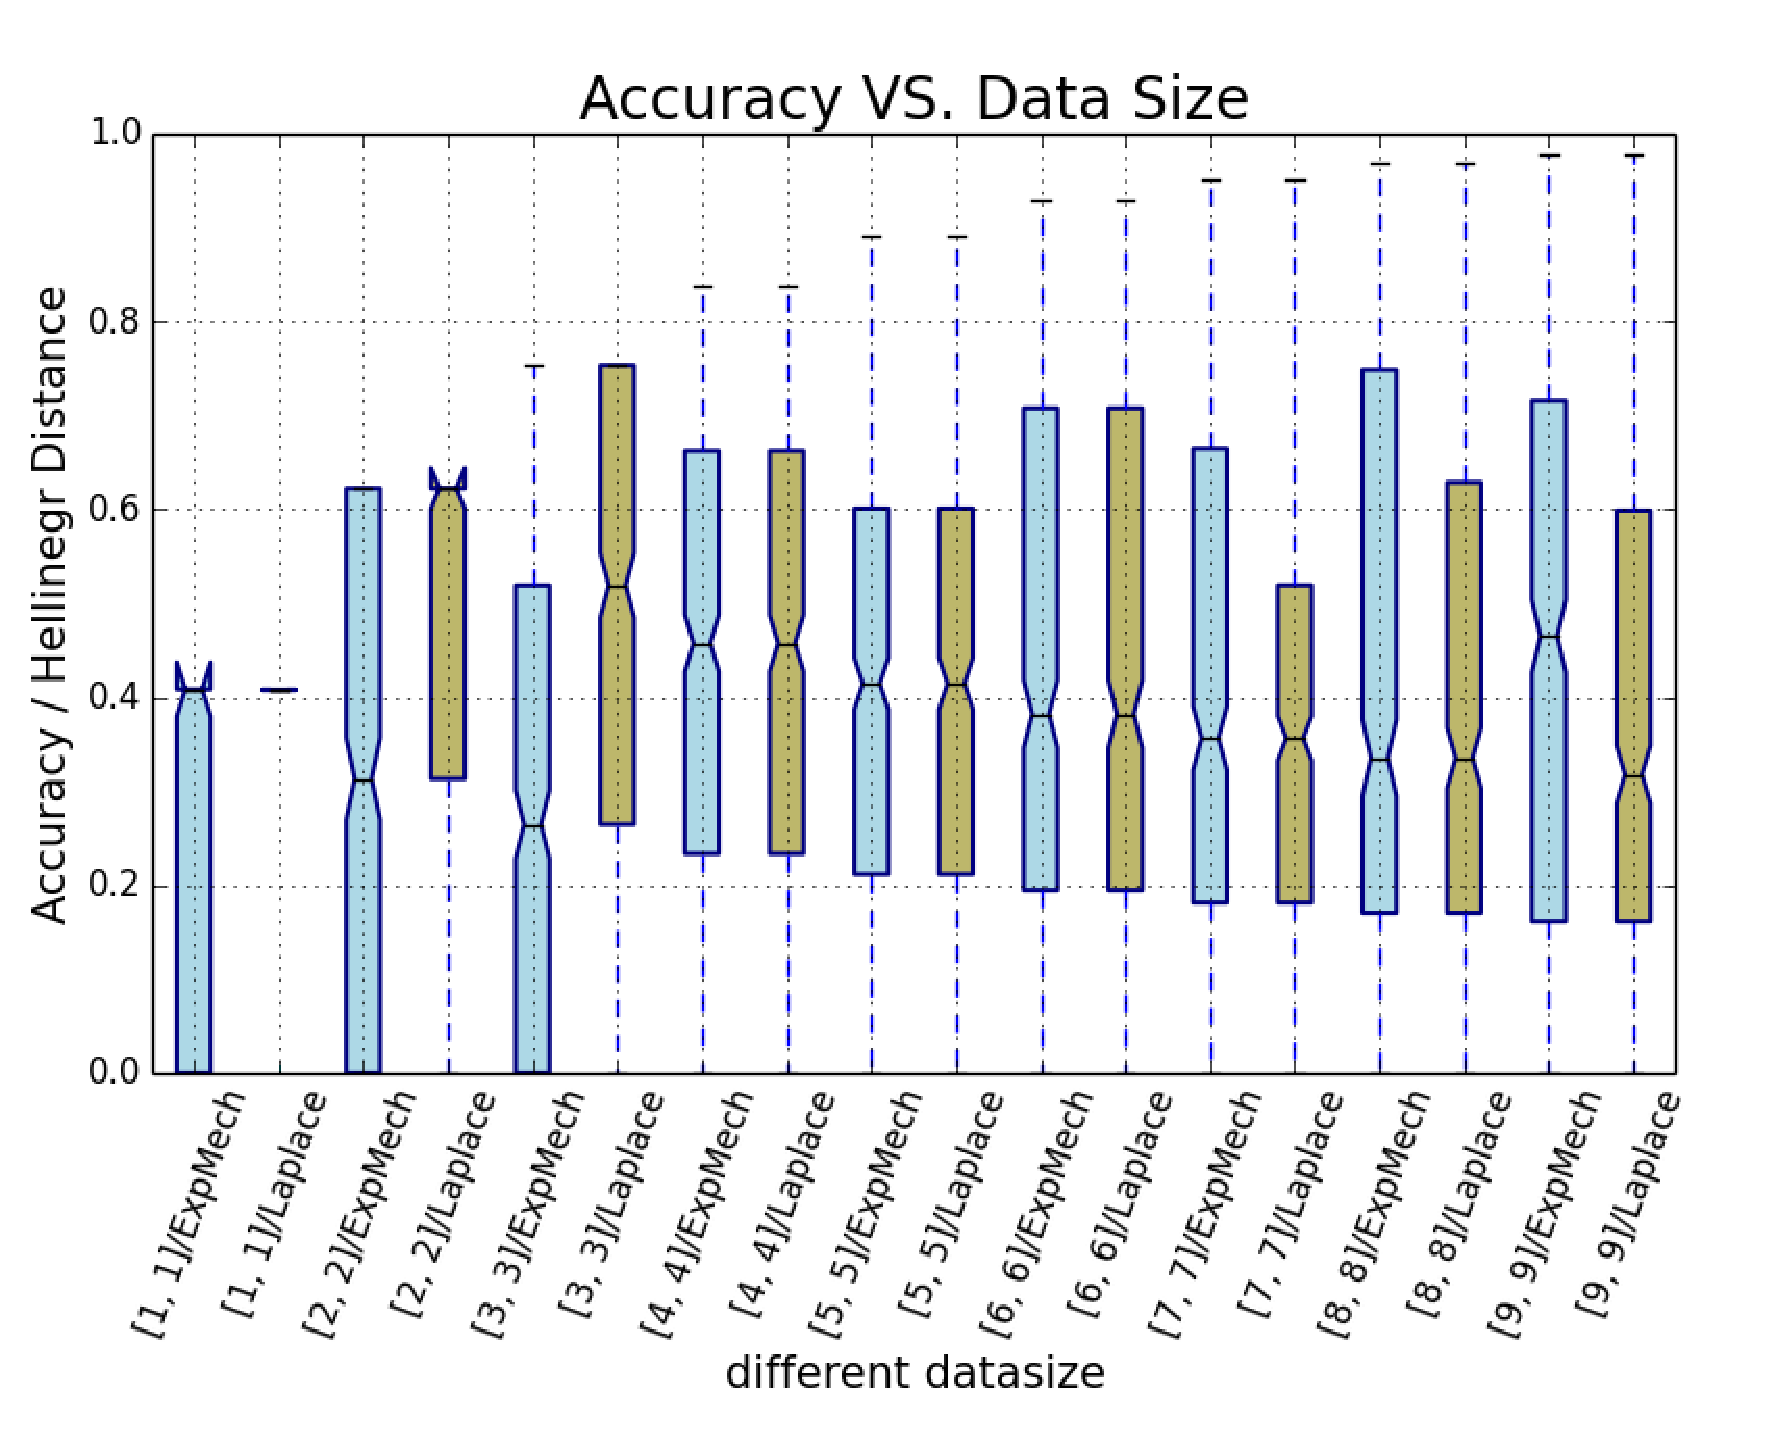
\includegraphics[width=0.3\textwidth]{accuracy_vs_datasize_1_1.eps}}
  \subfigure[three dimensions with $\dirichlet (1,1,1)$ prior distribution]{
    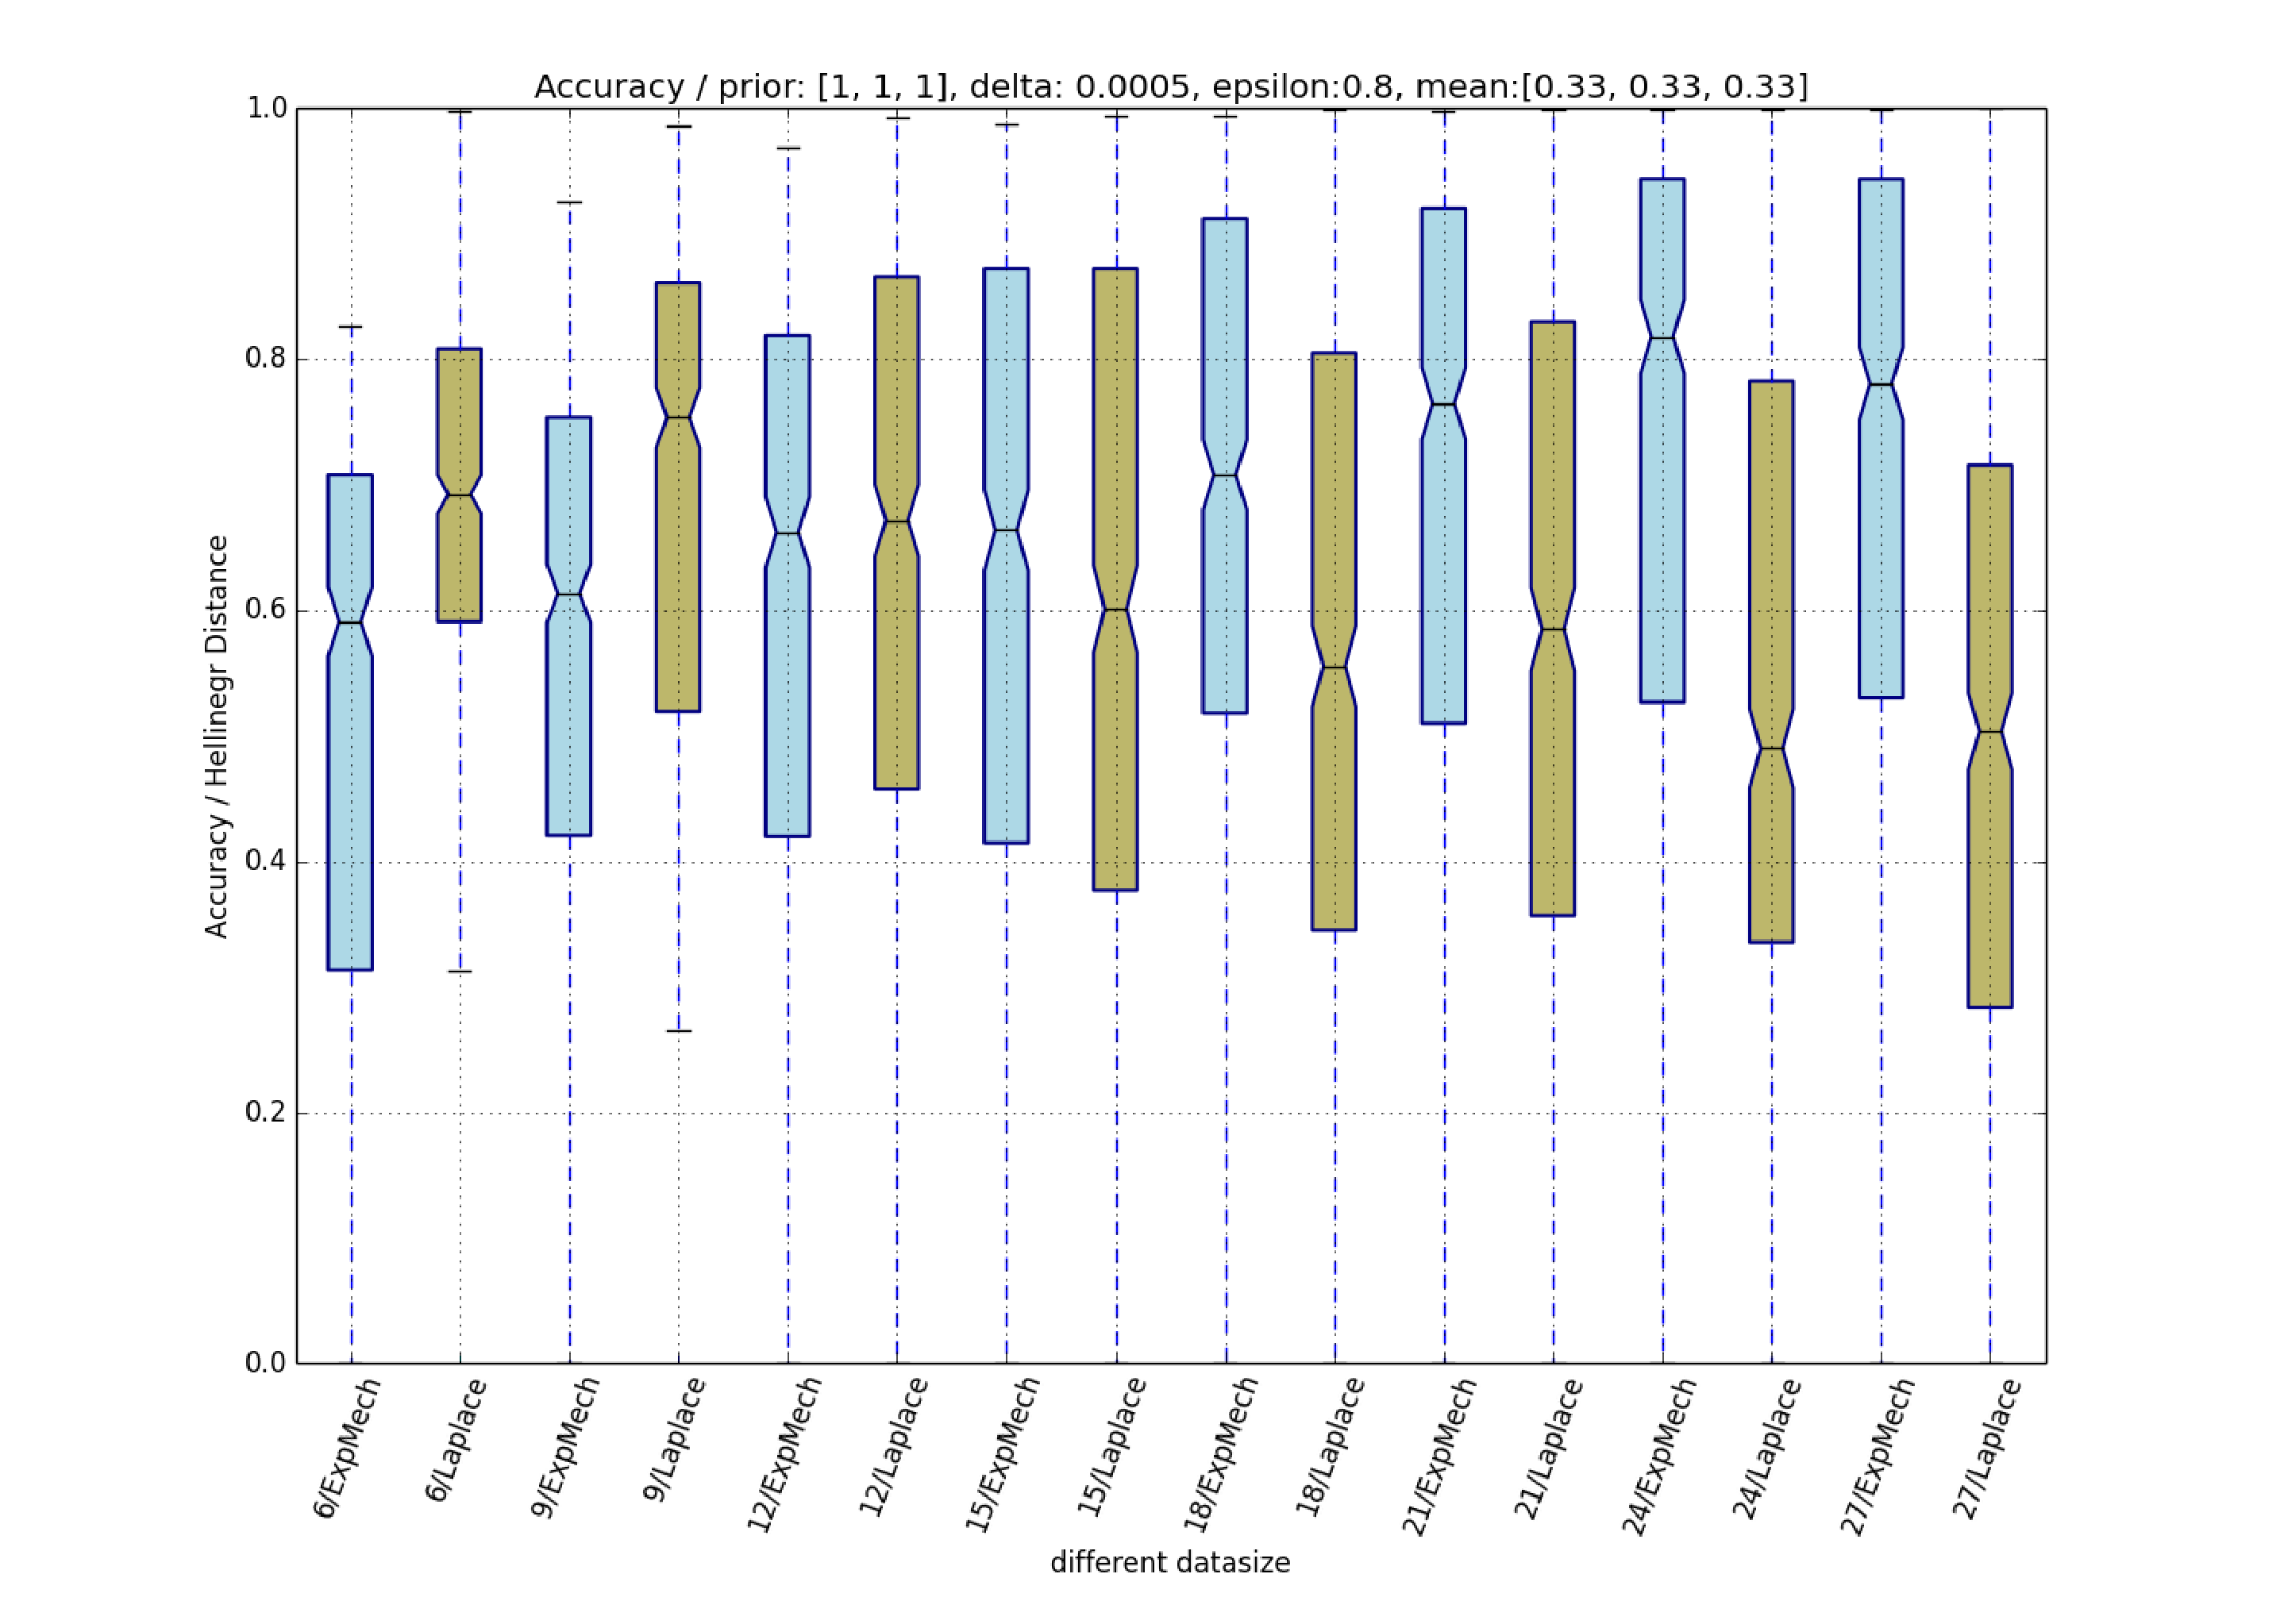
\includegraphics[width=0.3\textwidth]{accuracy_vs_datasize_1_1_1.eps}} 
\caption{Accuracy measurement based on Hellinger distance wrt. different datasizes. Settings: observed data are uniformly distributed, $\epsilon = 0.8$ and $\delta = 0.00000001$}
\label{fig_vs_datasize}
\end{center}
\end{figure}

In Fig. \ref{fig_vs_datasize}, both of the two plots show that when data size go larger, accuracy of our exponential mechanism are decreasing. In Fig. \ref{fig_vs_datasize}(a), when the data size is smaller than 12, we can beta Laplace mechanism but fail when data size larger than or equal to 12. Same as in Fig. \ref{fig_vs_datasize}(b), we can beat Laplace mechanism when data size is smaller than 15 and fail otherwise.

\subsubsection{Accuracy Evaluation wrt. Dimensions}
\label{subsubsec_vs_dimension}


\begin{figure}[ht]
\centering
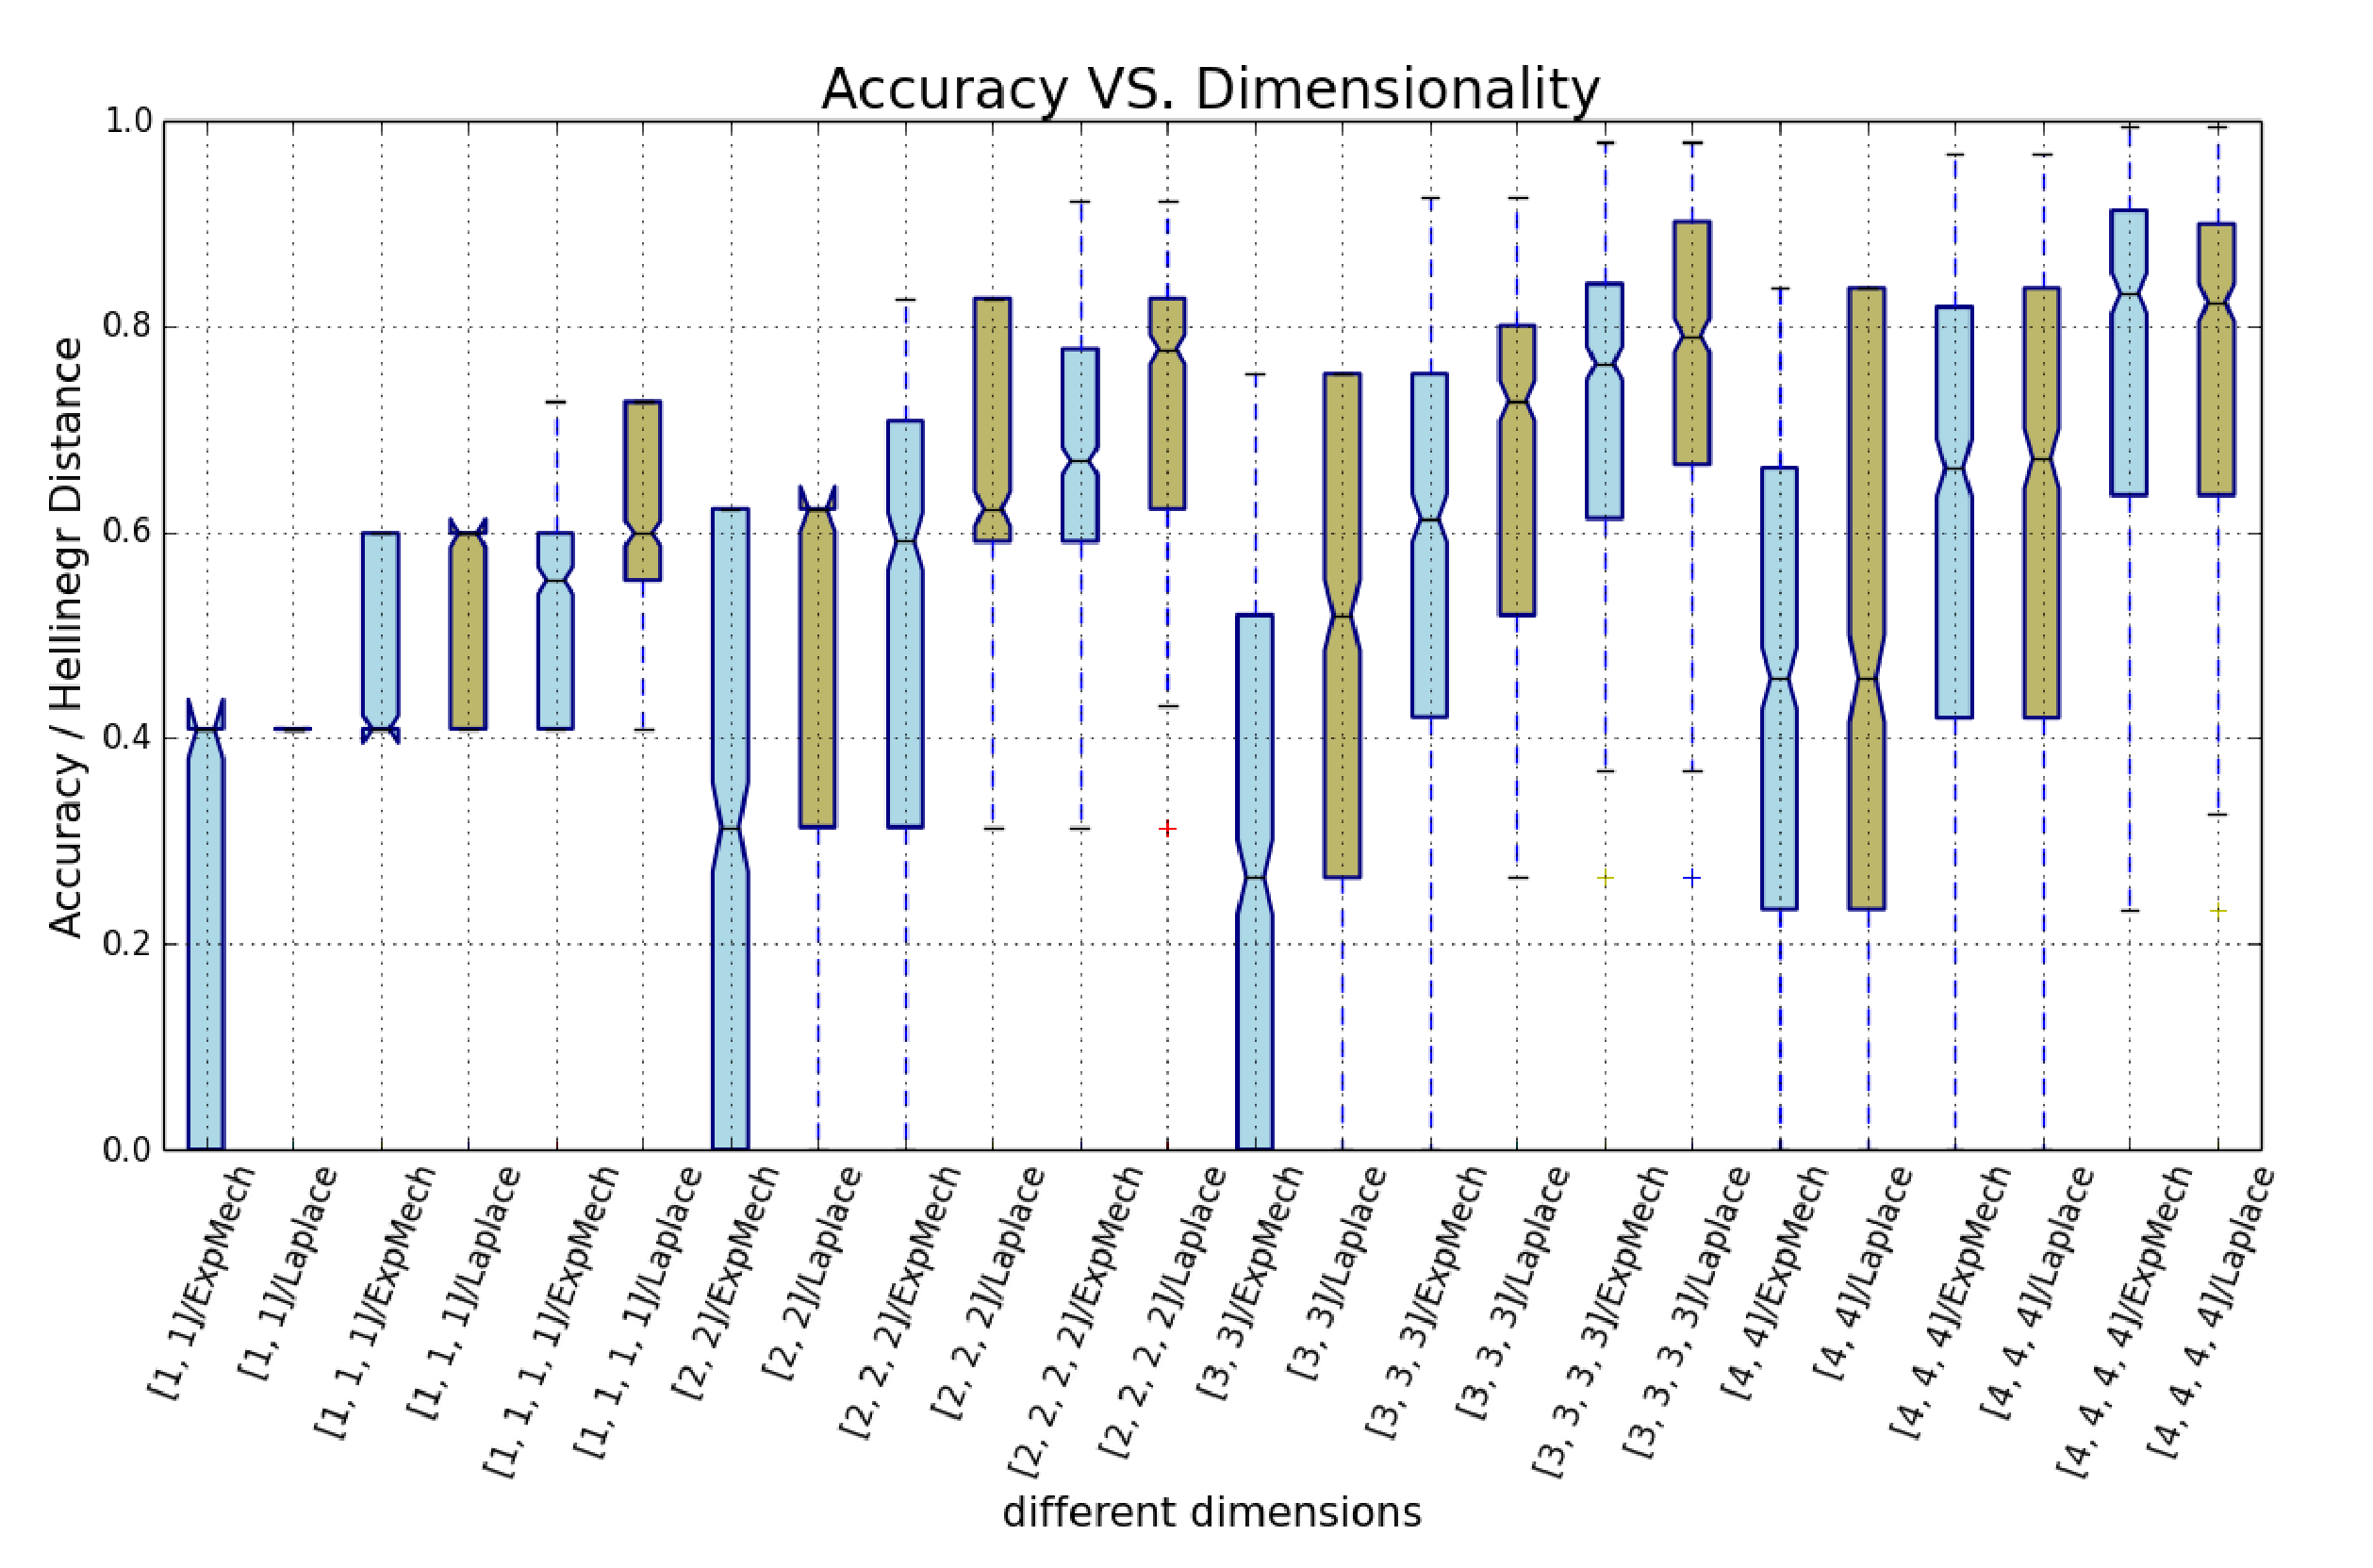
\includegraphics[width=0.45\textwidth]{accuracy_vs_dimension.eps}
\caption{Accuracy measurement based on Hellinger distance wrt. different dimensions and data size. Settings: observed data are uniformly distributed, $\epsilon = 0.8$ and $\delta = 0.00000001$, prior distributions are all $1$ in every dimension}
\label{fig_vs_dimension}
\end{figure}

In Fig. \ref{fig_vs_dimension}, x-axis are observed data sets of different size and dimensions. The plot shows that dimensions have similar influence on our exponential mechanism and the Laplace mechanism. Accuracy of two mechanisms both decrease when dimensions go larger. We will be beat by Laplace mechanism when data size increase but will not be affected when dimensions increase. In other words, dimension has little influence on whether we will beat Laplace mechanism.


\subsubsection{Accuracy Evaluation wrt. Data variance}
\label{subsubsec_vs_variance}

\begin{figure}[ht]
\centering
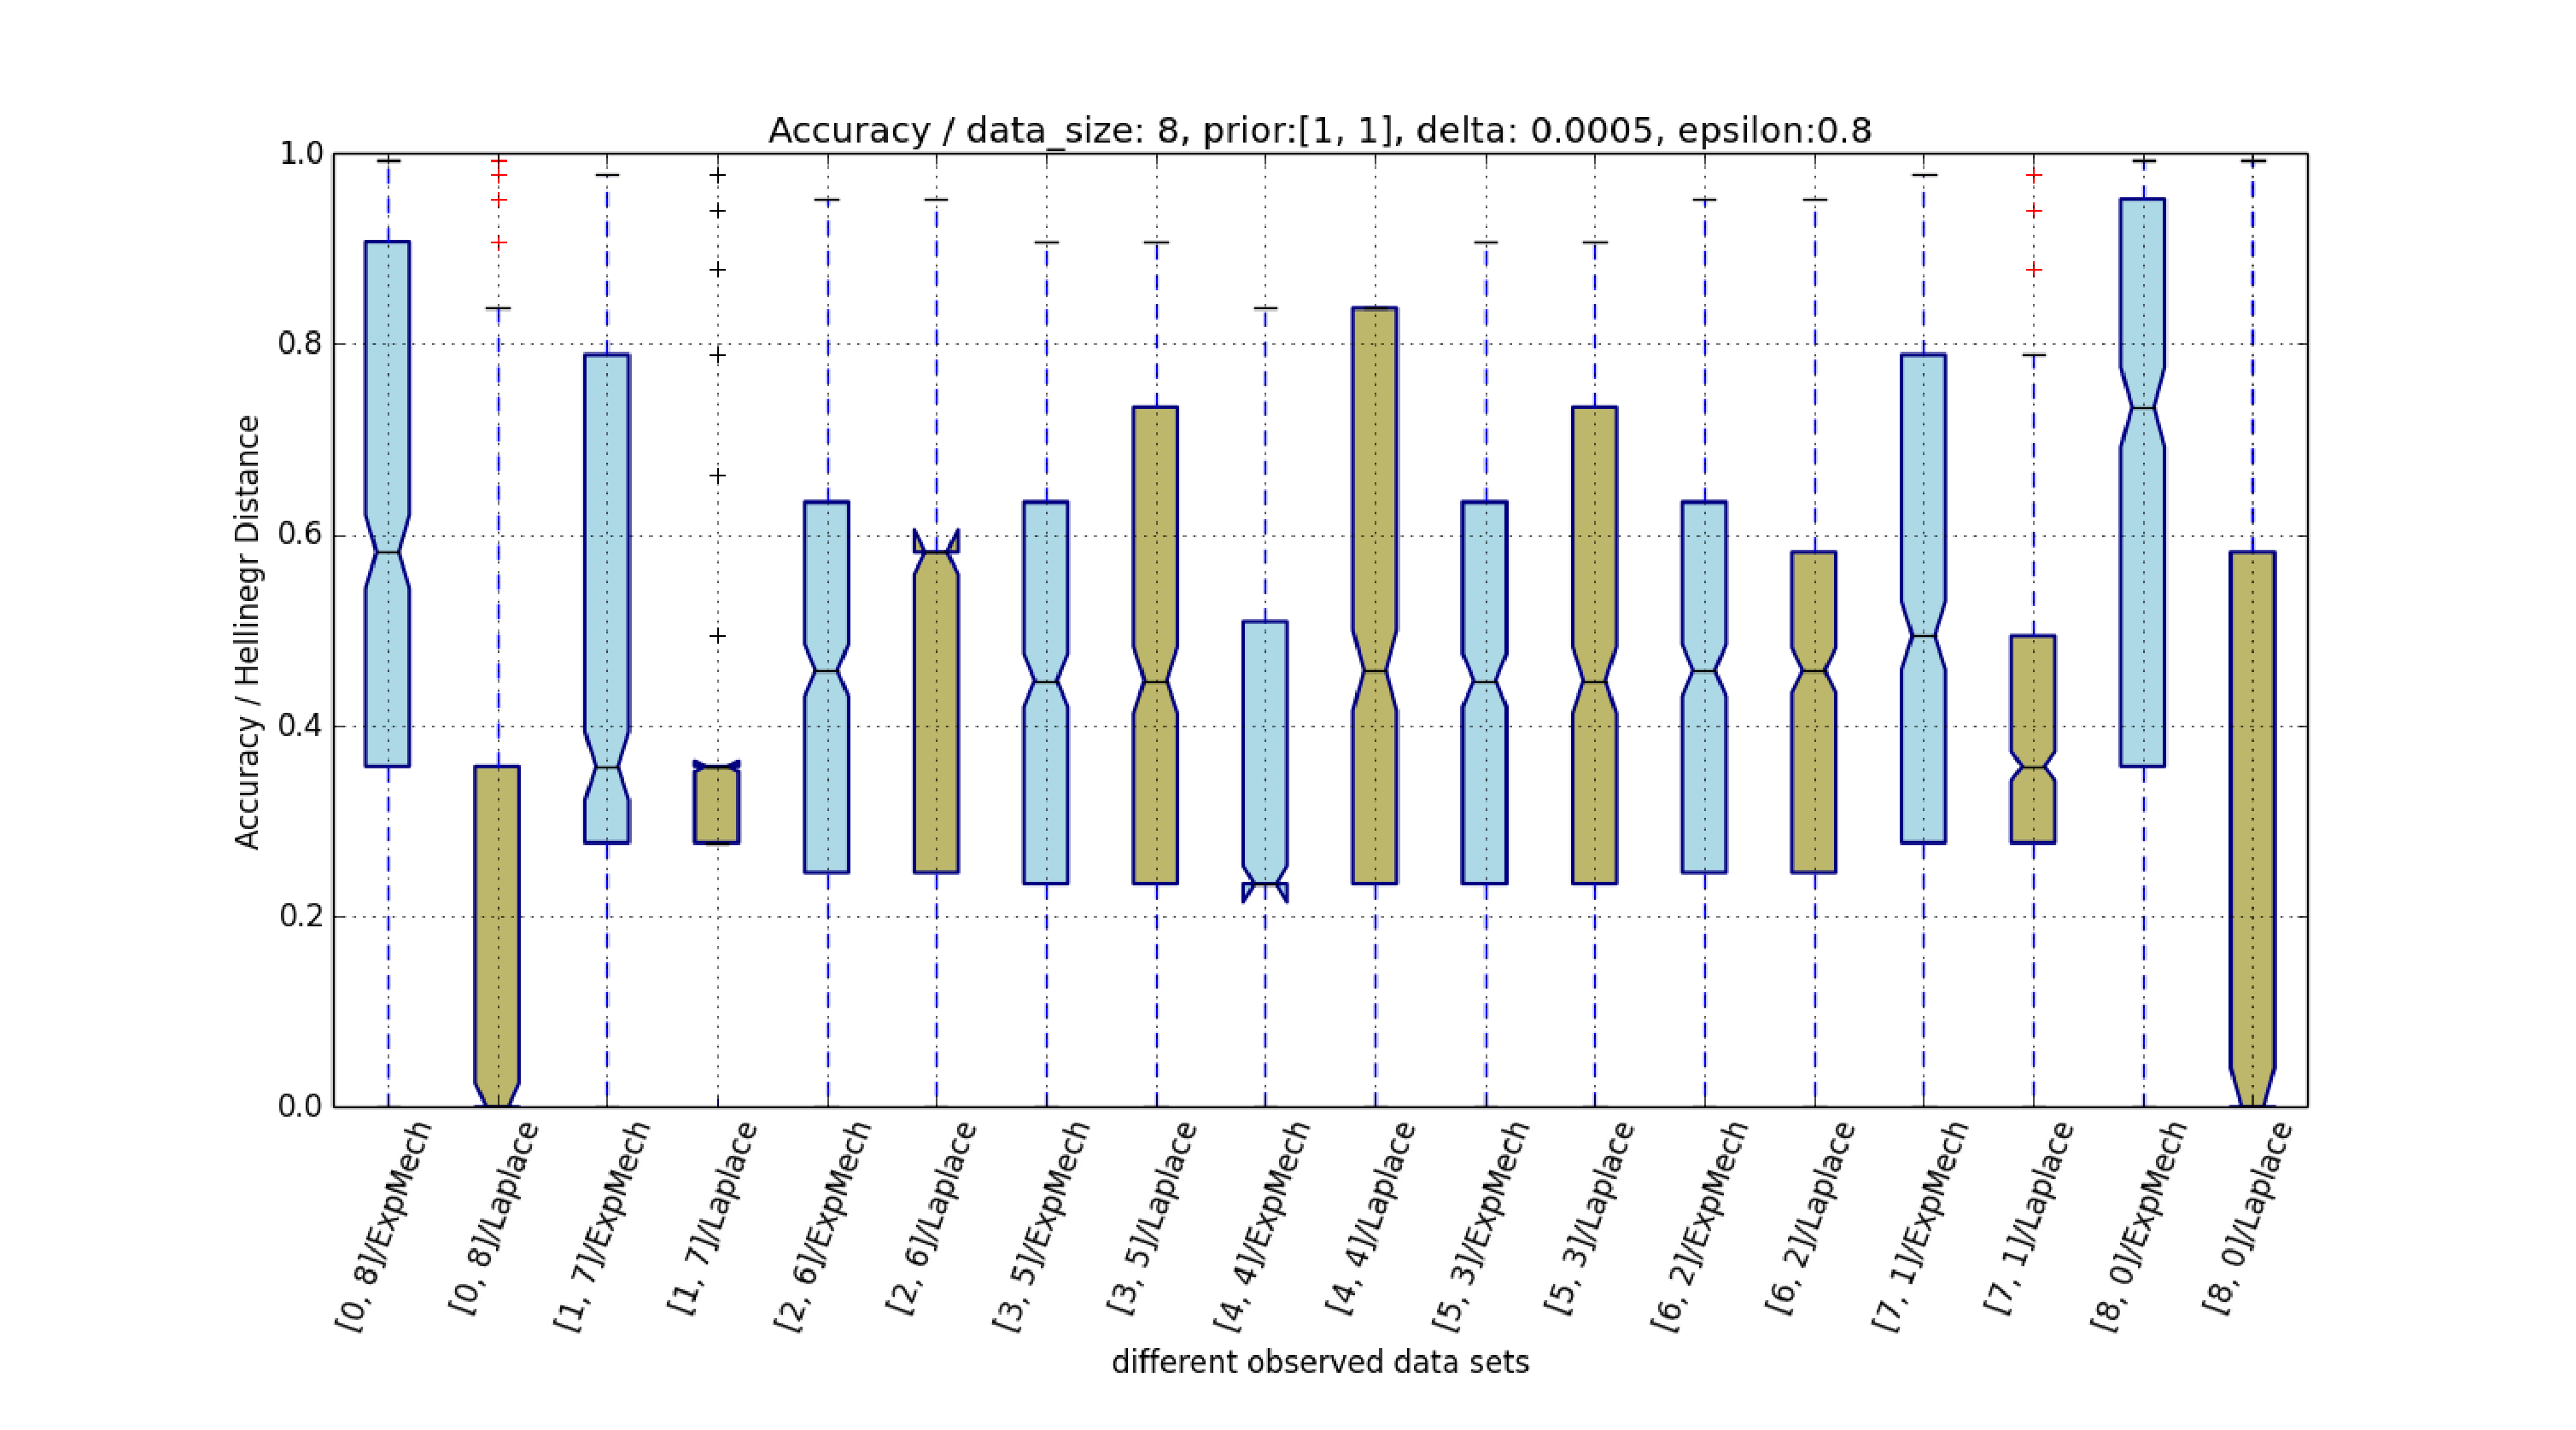
\includegraphics[width=0.45\textwidth]{accuracy_vs_mean_1_1.eps}
\caption{Accuracy measurement based on Hellinger distance wrt. different data variance. Settings: $\epsilon = 0.8$ and $\delta = 0.00000001$, prior distributions are all $1$ in every dimension}
\label{fig_vs_variance}
\end{figure}

In Fig. \ref{fig_vs_variance}, x-axis are observed data sets of different variances (or means). We study this variable under two-dimension $\betad$ distribution in order to be concise. It shows that our mechanism's accuracy is better when data variance go smaller, meanwhile Laplace mechanism go worse. We will beat Laplace mechanism when observed data are more uniformly.



\subsubsection{Accuracy Evaluation wrt. Prior Distribution}
\label{subsubsec_vs_prior}

\begin{figure}[ht]
\centering
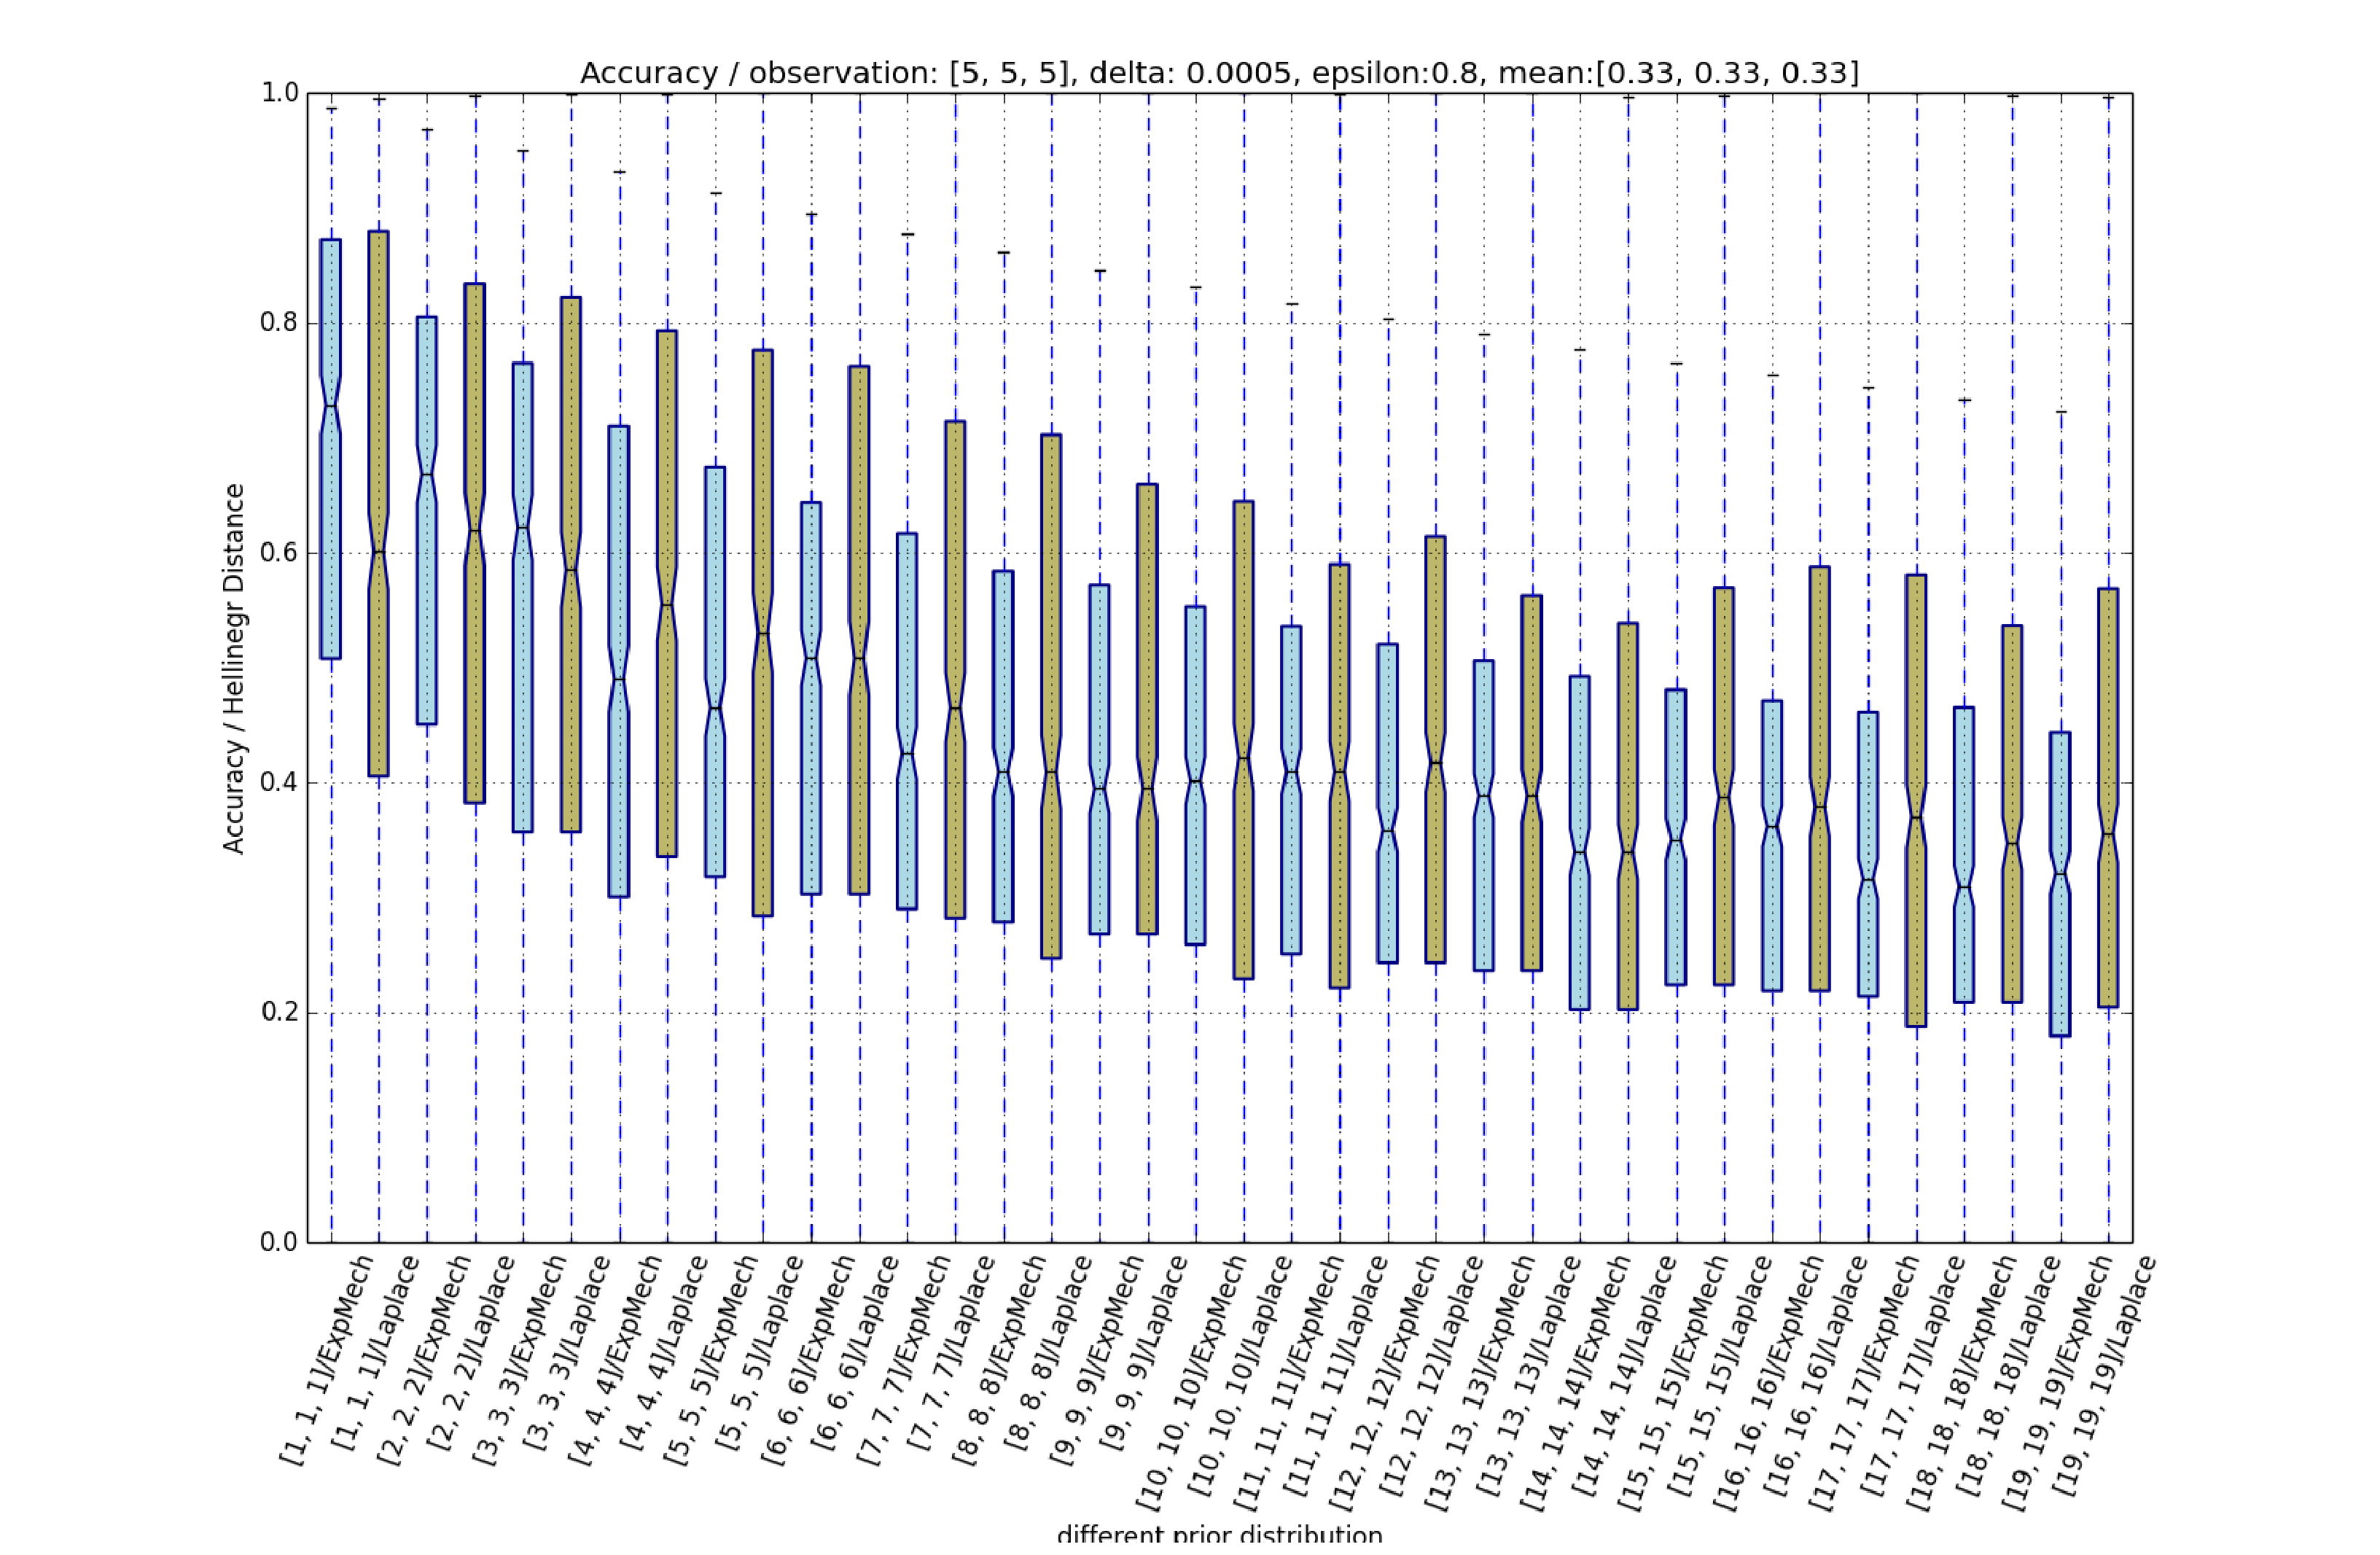
\includegraphics[width=0.45\textwidth]{accuracy_vs_prior_5_5_5.eps}
\caption{Accuracy measurement based on Hellinger distance wrt. different prior distribution. Settings: $\epsilon = 0.8$ and $\delta = 0.00000001$, observed data set is: $[5,5,5]$}
\label{fig_vs_prior}
\end{figure}

In Fig. \ref{fig_vs_prior}, we study this variable under setting that observed data set is $[5,5,5]$ because in Fig. \ref{fig_vs_datasize} Laplace mechanism beat us when data size is 15 and uniformly distributed. The plot shows that in the beginning we cannot beat Laplace but when prior distribution grow larger, we perform better and better and beat Laplace mechanism finally.



% \subsubsection{Accuracy Evaluation wrt. Prior Distribution and Data Variance}
% \label{subsubsec_vs_prior_variance}

% \begin{figure}[ht]
% \centering
% 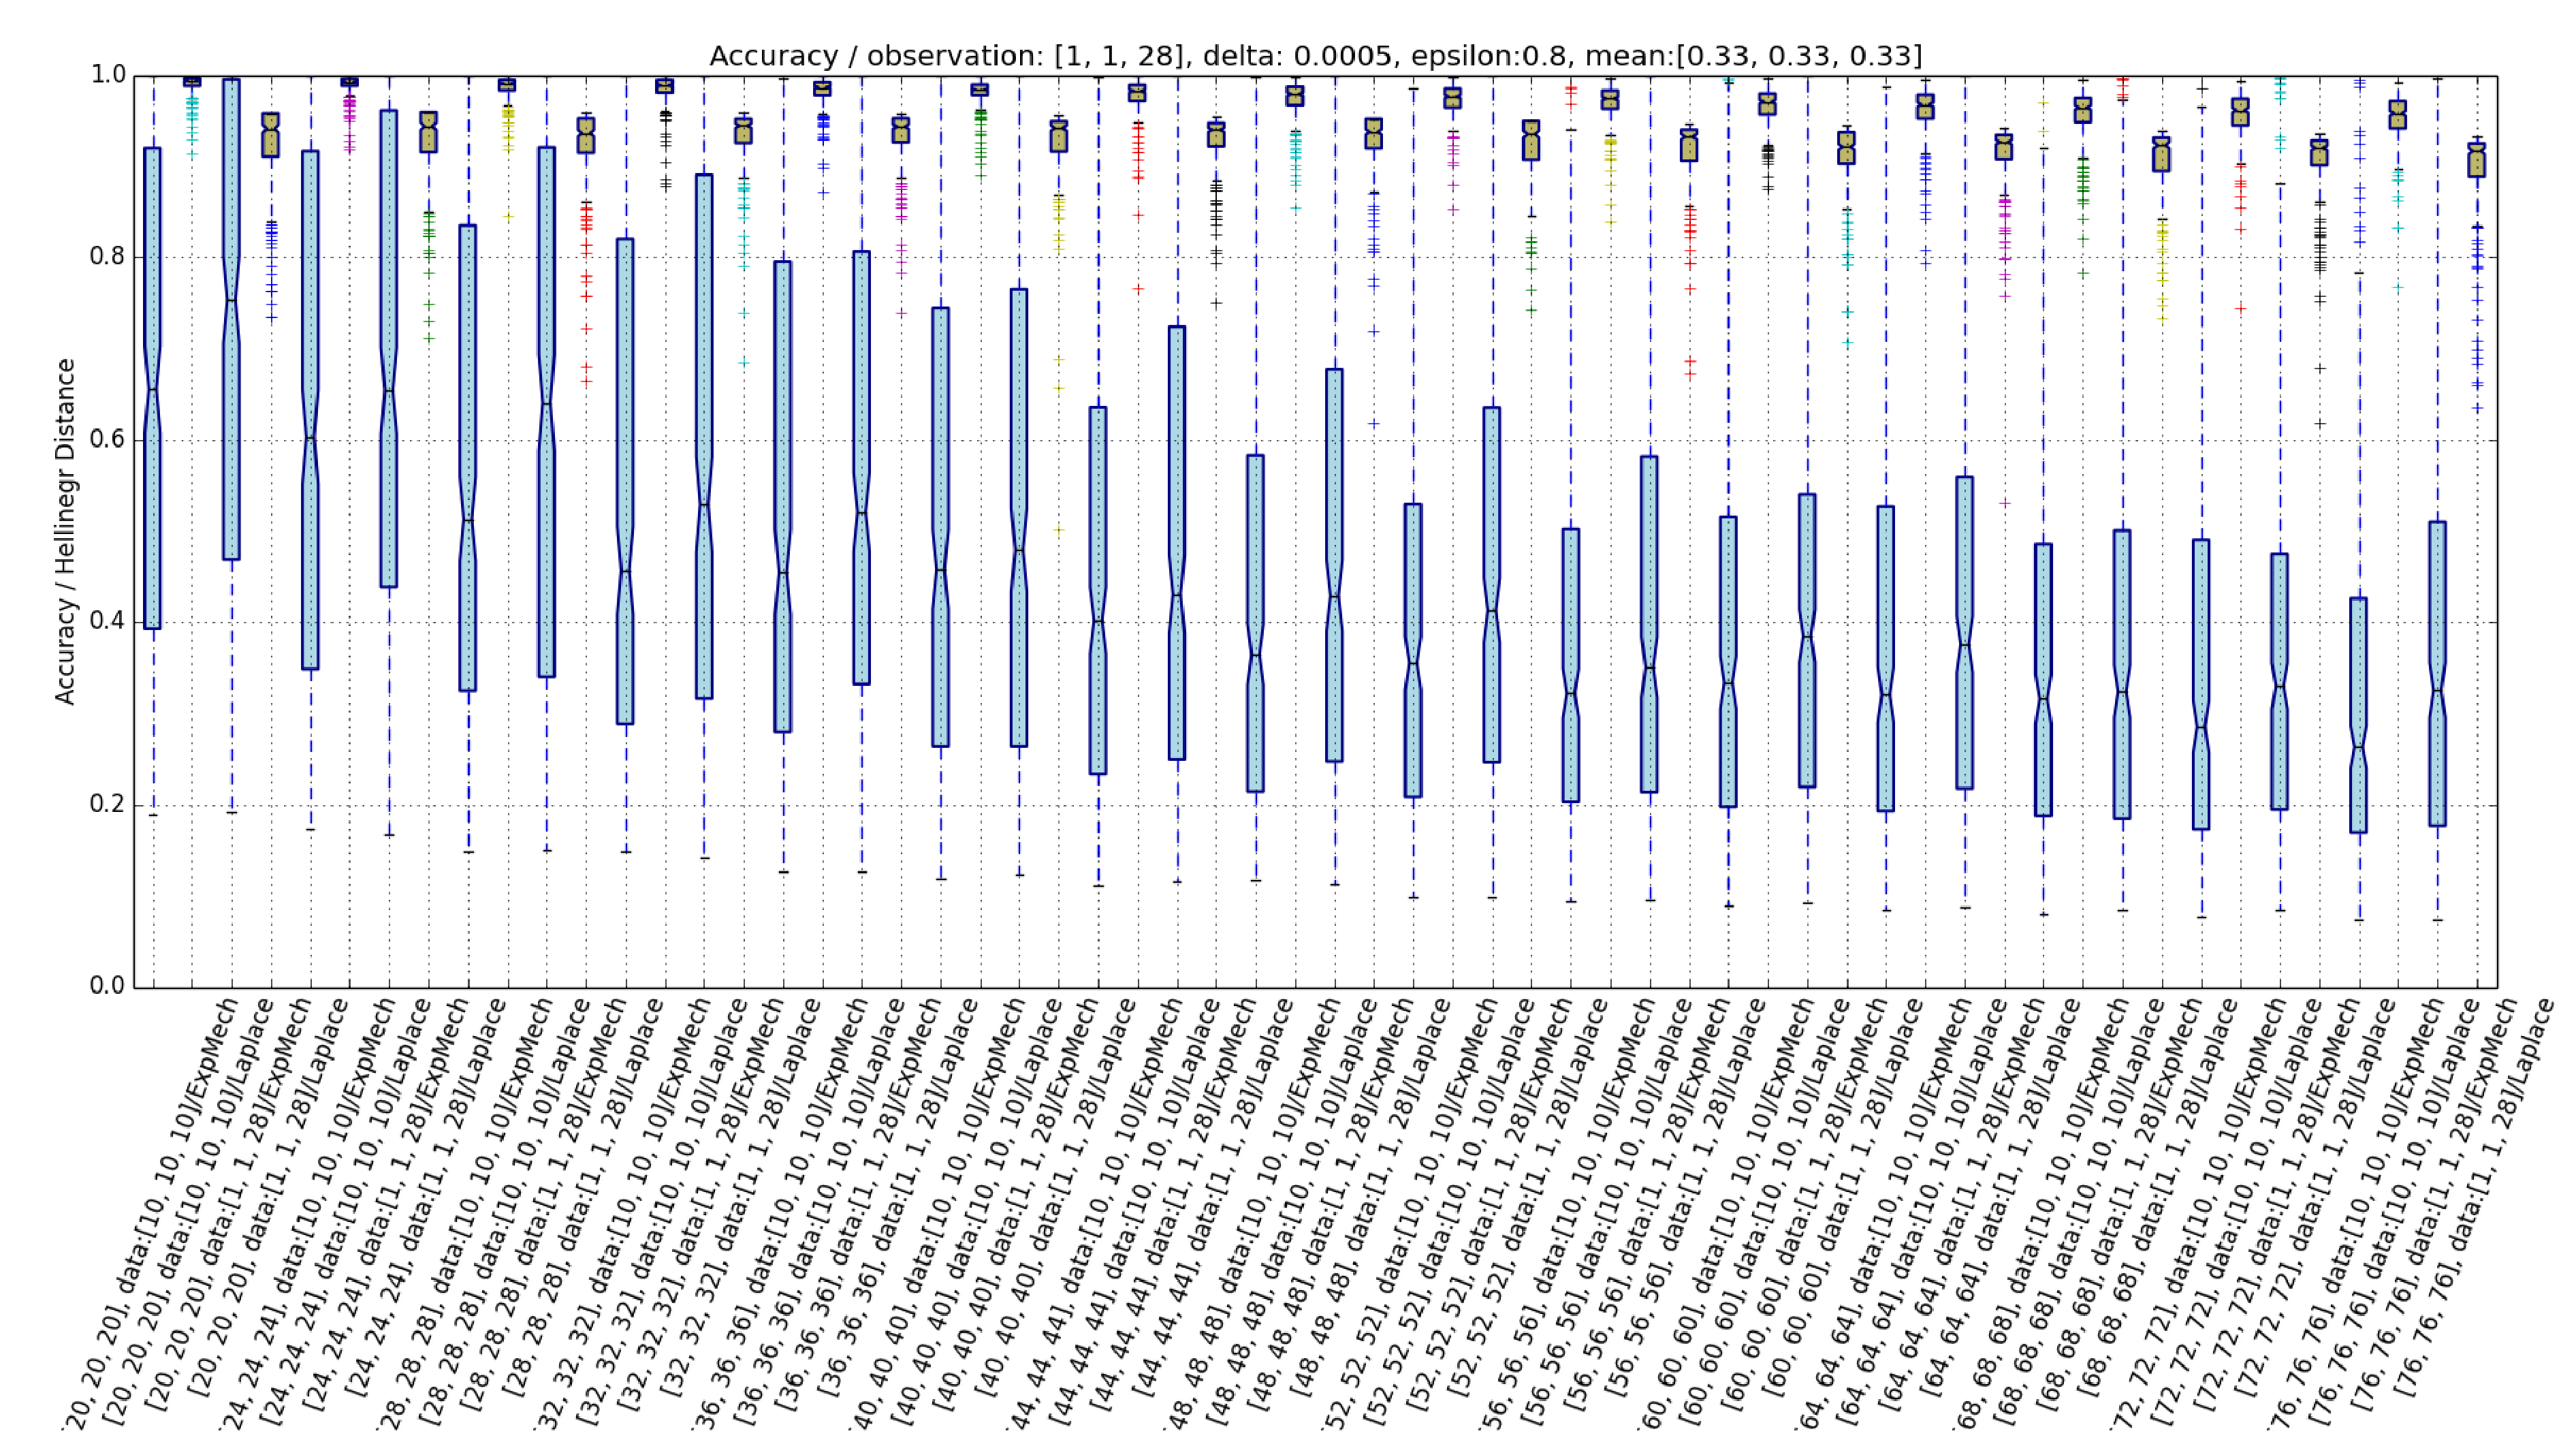
\includegraphics[width=0.45\textwidth]{Accuracy_VS_Prior_mean.eps}
% \caption{Accuracy measurement based on Hellinger distance wrt. different prior distribution and data variances. Settings: $\epsilon = 0.8$ and $\delta = 0.00000001$, observed data sets are $[10,10,10]$ and $[1,1,28]$ and prior distributions are range from $[20,20,20]$ to $[76,76,76]$}
% \label{fig_vs_prior_variance}
% \end{figure}

% Here, we change the prior distribution and data variance in the same time. As shown in Fig. \ref{fig_vs_prior_variance}, our exponential mechanism do better in uniform data set than in edging data set while Laplace mechanism on the contrary. Moreover, our mechanism is improving continuously and significantly as prior distribution increasing while Laplace mechanism isn't.


\section{Conclusions}
We can obtain some preliminary conclusions: 
\begin{enumerate}
	\item We can beat Laplace mechanism when data size is small.
	\item We will beat Laplace mechanism when observed data are more uniformly.
  \item When prior distribution grow larger, we perform better and better and beat Laplace mechanism finally.
\end{enumerate} 

In consequence, we have a better accuracy in small data size, in larger prior and in uniformly data.



\bibliographystyle{ACM-Reference-Format}
\bibliography{bayesian.bib}

\end{document}
 % TODO: replace with your brilliant paper!
% 
%packages
\usepackage{natbib}
\usepackage{amsmath}
\usepackage{amsthm}
\usepackage{mathtools}
\usepackage{mdframed}
\usepackage{subfigure}
\usepackage{booktabs}
% \usepackage{hyperref}
\usepackage{subfigure}
\usepackage{siunitx} % Provides the \SI{}{} and \si{} command for typesetting SI units
\usepackage{graphicx} % Required for the inclusion of images
% \usepackage{natbib} % Required to change bibliography style to APA
\usepackage{datetime}
\usepackage{lscape}
\usepackage{algorithm}
\usepackage{algorithmic}
\usepackage{xspace}
\usepackage[english]{babel} % English language/hyphenation
\usepackage{proof}
\usepackage{booktabs} % Top and bottom rules for tables
\usepackage[colorlinks, allcolors = blue,]{hyperref}
\usepackage{accents}
\usepackage{amsfonts}
\usepackage{stmaryrd}
\usepackage{amsmath,amsthm,amssymb,latexsym} 
\usepackage{microtype}
\usepackage{graphicx}
\usepackage{subfigure}
\usepackage{booktabs} % for professional tables
\usepackage{hyperref}
\usepackage{icml2019}
\usepackage{lipsum}

\usepackage{authblk}


%new commands
\newcommand{\theHalgorithm}{\arabic{algorithm}}
\newtheorem{definition}{Definition}
\usepackage{cancel}
\usepackage[normalem]{ulem}
\newcommand{\dataobs}{\textbf{x}}
\newcommand{\adj}[2]{\textbf{adj}(#1,#2)}
\newcommand{\candidateset}{\mathcal{R}_{\textup{post}}}
\newcommand{\bprior}{\boldsymbol{\beta}_{\textup{prior}}}
\newcommand{\bysinfer}{\mathsf{Infer}}
\newcommand{\betad}{\mathsf{Beta}}
\newcommand{\betaf}{\textup{B}}
\newcommand{\mbetaf}{\boldsymbol{\textup{B}}}
\newcommand{\vtheta}{\boldsymbol{\theta}}
\newcommand{\valpha}{\boldsymbol{\alpha}}
\newcommand{\vbeta}{\boldsymbol{\beta}}
\newcommand{\lapmech}{\mathsf{LSDim}}
\newcommand{\ilapmech}{\mathsf{LSHist}}
\newcommand{\binomial}[2]{\mathsf{Bin}(#1, #2)}
\newcommand{\multinomial}[2]{\mathsf{Mult}(#1, #2)}
\newcommand{\expmech}{\mathsf{EHD}}
\newcommand{\hexpmech}{\mathsf{EHDS}}
\newcommand{\lexpmech}{\mathsf{EHDL}}
\newcommand{\hexpmechd}{\mathsf{expMech}^{D}_{\hellinger}}
\newcommand{\privinfer}{\mathsf{PrivInfer}}
\newcommand{\hlg}{\mathsf{H}}
\newcommand{\dirichlet}[1]{\mathsf{Dir}(#1)}
\newcommand{\alphas}{\boldsymbol{\alpha}}
\newcommand{\xis}{\boldsymbol{\xi}}
\newcommand{\iverson}[1]{[#1]}
\newcommand{\datauni}{\mathcal{X}}
\newcommand{\hellinger}{\mathcal{H}}
\newcommand{\ux}[1]{u(\textbf{x}, {#1})}
\newcommand{\uxadj}[1]{u(\textbf{x}', {#1})}
\newcommand{\cardinality}[2]{\mathcal{C}^{#1}_{#2}}
\newcommand{\range}{\mathcal{O}}
\newcommand{\nomalizer}[1]{\sum\limits_{r'\in \mathcal{R}_{\textup{post}}} \exp \big(\frac{-\epsilon\cdot \mathcal{H} (\mathsf{BI}(#1),r')}{4 \cdot S(#1)}\big)}

\newcommand{\unomalizer}[1]{\sum\limits_{r'\in \mathcal{R}_{\textup{post}}} \exp \big(\frac{-\epsilon\cdot u(#1, r')}{4 \cdot S(#1)}\big)}


\newcommand{\hexpmechPr}[2]{\underset{z \thicksim \hexpmech(#1)}{\Pr}\left[ #2 \right]}
\newcommand{\lapmechPr}[2]{\underset{z \thicksim \lapmech(#1)}{\Pr}\left[ #2 \right]}

\newcommand{\ilapmechPr}[2]{\underset{
{z \thicksim \ilapmech(#1)}
}{\Pr}\left[ #2 \right]}

\newtheorem{thm}{Theorem}[section]

\newtheorem{lem}{Lemma}[section]

\newtheorem{assert}{Assertion}[lem]
\newcommand{\lap}[2]{\mathsf{Lap}(#1, #2)}
\newcommand{\todo}[1]{{\footnotesize \color{red}\textbf{[[ #1 ]]}}}

\section{Bayesian Inference Background}
Given a prior belief $\Pr(\theta)$ on some parameter $\theta$,
and given an observation $\dataobs$,
the posterior distribution on $\theta$ given $\dataobs$ is computed as:
\[
  \Pr(\theta | \dataobs) = \frac{Pr(\dataobs | \theta) \cdot \Pr(\xis)}{\Pr(\dataobs)}
\]
where the expression  $\Pr(\dataobs | \theta)$ denotes the \emph{likelihood} of $\theta$ when
\dataobs~ is observed. Since we consider \dataobs to be fixed the likelihood is a function of $\theta$.
For the same reason $\Pr(\dataobs)$ is a constant independent of $\theta$.
Usually in statistics the prior distribution $\Pr(\theta)$ is chosen so that it represents
the initial belief on $\theta$. That is, when no data has been observed. In practice though,
prior distributions and likelihood functions are usually chosen so that the posterior
belongs to the same \emph{family} of distributions. In this case we say that the prior
is conjugate of the likelihood function. Using conjugate priors simplify calculcations and allows
for inference to be performed in a recursive fashion over the data.
In this work we will consider a specific instance of Bayesian inference and one of its generalizations.
Specifically, we will consider the situation where $\theta$ represents the parameter --informally called \emph{bias})--
of a Bernoulli distributed random variable, and its immediate generalization where the parameter $\vtheta$ represents
the the vector of parameters of a categorical distributed random variable.
In the former case the prior distribution over $\theta\in [0,1]$ is going to be a beta distribution, $\betad(\alpha, \beta)$, with parameters
$\alpha,\beta\in\mathbb{R}^{+}$, and with p.d.f:
\[
  \Pr(\theta)\equiv \frac{\theta^{\alpha} (1- \theta)^{\beta}}{\betaf(\alpha,\beta)}
\]
where $\betaf(\cdot,\cdot)$ is the beta function.
The data $\dataobs$ will be a sequence of $n\in\mathbb{N}$ 0/1 values, that is $\dataobs=\ll x_1,\dots x_n \gg, x_i\in\{0,1\}$, and the likelihood function is:
\[
  \Pr(\dataobs | \theta)\equiv \theta^{a}(1-\theta)^{n-a}
\]
where $a=\displaystyle\sum_{i=1}^{n}\mathrm{x_i}$.
From this it can easily be derived that the posterior distribution is:
\[
  \Pr(\theta|\dataobs)=\betad(\alpha+a,\beta+n-a)
\]
In the latter case the prior distribution over $\vtheta\in [0,1]^{k}$ is given by a Dirichelet distribution, $\dirichlet(\vtheta)$, for $k\in\mathbf{N}$,
and $\valpha\in(\mathbf{R^{+}})^{k}$, with p.d.f:
\[
  \Pr(\vtheta)\equiv\frac{1}{\mbetaf(\valpha)}\cdot \displaystyle\prod_{i=1}^{k}{\theta_i^{\alpha_i-1}}
\]
where $\mbetaf(\cdot)$ is the generealised beta function.
The data $\dataobs$ will be a sequence of $n\in\mathbb{N}$ values coming from a universe $\datauni$, such that $\mid\datauni \mid=k$.
The likelihood function will be:
\[
  \Pr(\dataobs|\vtheta)\equiv \displaystyle\prod_{a\in\datauni}\alpha_{a}^{z_a}
\todo{to check}\]
where $z_a=\displaystyle\sum_{i=1}^{n}\iverson{x_i=a}$, where in $\iverson{\cdot}$ we use
Iverson bracket notation. The posterior distribution over $\vtheta$ turns out to be
\[
  \Pr(\vtheta|\dataobs)=\todo{to type down}\dirichlet(\vtheta+...)
\]
\section{Problem Statement}
% When we try
% to make this distribution public, sensitive information of the data
% based on which the posterior drew from can be compromised. So, it is
% important to protect this posterior distribution. When our protection
% objective is a distribution rather than a numeric value or vector, it
% would be better to measure the accuracy by distance over
% distributions, for instance, Hellinger distance, than by numeric
% metrics like $\ell_1$-norm.
This work will show that the same mechanism can
perform differently when its accuracy is computed w.r.t to a metric
over probability measures (e.g total variation distance, or Hellinger distance)
from when the metric (e.g. $\ell_1$-norm) is over the parameters.  
\section{Technical Problem Statement}
\label{sec_bayesInfer}
The posterior belief about parameters $\xis$ is inferred from the
group of sensitive data. Because it is usually published in form of a
distribution, for example, $\betad(\alpha',\beta'), \cdots,$ itself
can relieve a lot of information about sensitive data. So, the
sensitive information we want to protect here is the posterior belief,
i.e., $Pr(\xis | \dataobs)$, rather than just a sample drew from
it\cite{foulds2016theory}. Then it will be better if we can use a
distance over two distributions to measure the accuracy than a
distance over just parameters or values when we are protecting a
distribution, for instance, Hellinger distance in our paper. When we
measure the accuracy between true posterior and protected posterior
using Hellinger distance, it would be better we can have a protection
mechanism based on Hellinger distance. However, current mechanisms are
mainly based on $l_1$ norm by Laplace mechanism
\cite{zhang2016differential} \cite{xiao2012bayesian}. That's why we
design our exponential mechanism over Hellinger distance to protect
the whole posterior distribution.


\section{Baseline Approach - Laplace Mechanism}
\label{sec_lap}
Based on the posterior results from Bayesian inference, we calculate the Laplace mechanism updates on posterior and get the private results under Laplace mechanism. In the case of $m$ dimension Dirichlet distribution, we will add $(m-1)$ i.i.d. Laplace noises $\{| Lap_1 |, | Lap_2 |, \cdots, | Lap_{m-1} |\}$ to the output, where $Lap_i = floor(Y)$, $Y \sim Lap(\frac{2}{\epsilon})$. The private posterior then will be $\dirichlet(\alpha_1 + n_1 + | Lap_1 |, \alpha_2 + n_2 + | Lap_2 |, \cdots, \alpha_m + n - (Lap_1 + \cdots + Lap_{m-1}))$.

\section{Our Approach - Exponential Mechanism with Smooth Sensitivity}
\label{sec_smoo}

% \subsection{Algorithm Setting up}
We define a new mechanism $\hexpmech(x)$ which is similar to the exponential mechanism where we use $\mathcal{R}$ as the set $\betaset$ of beta distributions with integer parameters summing up to $n+2$, as scoring function we use the Hellinger distance from $\bysinfer(x)$, i.e. $\hlg(\bysinfer(x),-)$, and we calibrate the noise to the smooth sensitivity~\cite{nissim2007smooth}. The only difference is in the sensitivity part, since now we use the smooth sensitivity.

\begin{definition}
\label{def_smoo}
The mechanism $\hexpmech(x)$ outputs a candidate $r \in \betaset$ with probability
\begin{equation*}
\underset{z \thicksim \hexpmech(x)}{Pr}[z=r] = \frac
{exp(\frac{-\epsilon\hlg(\bysinfer(x),r)}{2 S_\beta(x)})}
{\Sigma_{r' \in R}\ exp(\frac{-\epsilon \hlg(\bysinfer(x),r')}{2 S_\beta(x)})},
\end{equation*}
where $s_\beta(x)$ is the smooth sensitivity of $\hlg(\bysinfer(x),-)$, calculated by:
\begin{equation*}
S_{\beta}(x) = \max(\Delta_{l}\hlg(\bysinfer(x),-), \max_{y \neq x; y \in D^{n}}(\Delta_{l}\hlg(\bysinfer(y),-)\cdot e^{-\beta d(x,y)})),
\end{equation*}
where $d$ is the Hamming distance between two datasets, and $\beta =
\beta(\epsilon, \delta)$ is a function of $\epsilon$ and $\delta$. 
\end{definition}


In what follows, we will use a correspondence between the probability
 $\underset{z \thicksim \hexpmech(x)}{Pr}[z = r]$ of every
 $r\in\betaset$ and the probability 
 $\underset{z \thicksim \hexpmech(x)}{Pr}[\hlg(\bysinfer(x),z) =
 \hlg(\bysinfer(x),r)]$ for the utility score for $r$. In particular, for every
 $r\in\betaset$ we have:
$$
\underset{z \thicksim \hexpmech(x)}{Pr}[z = r]=
\frac{1}{2}\Big (\underset{z \thicksim \hexpmech(x)}{Pr}[\hlg(\bysinfer(x),z) =
 \hlg(\bysinfer(x),r)]\Big )
$$
To see this, it is enough to notice that: $\underset{z \thicksim \hexpmech(x)}{Pr}[z = r]$ is proportional too $\hlg(\bysinfer(x),r)$, i.e., $u(x,z)$. We can derive, if $u(r,x) = u(r',x)$ then $\underset{z \thicksim \hexpmech(x)}{Pr}[z = r] = \underset{z \thicksim \hexpmech(x)}{Pr}[z = r']$. We assume the number of candidates $z \in \mathcal{R}$ that satisfy $u(z,x) = u(r,x)$ is $|r|$, we have  $\underset{z \thicksim \hexpmech(x)}{Pr}[u(z,x) = u(r,x)] = |r| \underset{z \thicksim \hexpmech(x)}{Pr}[z = r]$. Because Hellinger distance  $\hlg(\bysinfer(x),z)$ is axial symmetry, where the $\bysinfer(x)$ is the symmetry axis. It can be infer that $|z| = 2$ for any candidates, apart from the true output, i.e., $\underset{z \thicksim \hexpmech(x)}{Pr}[u(z,x) = u(r,x)] = 2 \underset{z \thicksim \hexpmech(x)}{Pr}[z = r]$. This parameter can be eliminate in both sides in proof.

In our private Bayesian inference mechanism, we set the $\beta$ as $\ln(1 - \frac{\epsilon}{2 \ln (\frac{\delta}{2 (n + 1)})})$. 





% \subsection{Sliding Property of Exponential Mechanism}
% \begin{lem}
% Consider the exponential mechanism  $\sexpmech(x,u,\mathcal{R})$
% calibrated on the smooth sensitivity. Let $\lambda = f(\epsilon,
% \delta)$, $\epsilon\geq 0$ and $|\delta| < 1$. Then, the following \emph{sliding property} holds:
% \begin{equation*}
% \underset{r \thicksim \hexpmech(x)}{Pr}[u(r,x) = \hat{s}]
% \leq
% e^{\frac{\epsilon}{2}} \underset{r \thicksim \hexpmech(x)}{Pr}[u(r,x) = (\Delta + \hat{s})] + \frac{\delta}{2},
% \end{equation*}

% \end{lem}

% \begin{proof}

% We denote the normalizer of the probability mass in $\hexpmech(x)$: $\sum_{r' \in \mathcal{R}}exp(\frac{\epsilon u(r',x)}{2 S(x)})$ as $NL(x)$:
% \begin{equation*}
% \begin{split}
% LHS 
%   = \underset{r \thicksim \hexpmech(x)}{Pr}[u(r,x) = \hat{s}]
% & = \frac{exp(\frac{\epsilon \hat{s}}{2 S(x)})}{NL(x)}\\
% & = \frac{exp(\frac{\epsilon (\hat{s} + \Delta - \Delta)}{2 S(x)})}{NL(x)}\\
% & = \frac{exp(\frac{\epsilon (\hat{s} + \Delta)}{2 S(x)} + \frac{- \epsilon \Delta}{2 S(x)})}{NL(x)}\\
% & = \frac{exp(\frac{\epsilon (\hat{s} + \Delta)}{2 S(x)})}{NL(x)} \cdot e^{\frac{- \epsilon \Delta}{2 S(x)})}.\\
% \end{split}
% \end{equation*}

% By bounding the $\Delta \geq -S(x)$, we can get:

% \begin{equation*}
% \begin{split}
% \frac{exp(\frac{\epsilon (\hat{s} + \Delta)}{2 S(x)})}{NL(x)} \cdot e^{\frac{- \epsilon \Delta}{2 S(x)}}
% & \leq \frac{exp(\frac{\epsilon (\hat{s} + \Delta)}{2 S(x)})}{NL(x)} \cdot e^{\frac{\epsilon}{2}}\\
% &  =  e^{\frac{\epsilon}{2}} \underset{z \thicksim \hexpmech(x)}{Pr}[u(r,x) = (\Delta + \hat{s})] \leq RHS\\
% \end{split}
% \end{equation*}

% \end{proof}

% \subsection{Dilation Property of Exponential Mechanism}
% \begin{lem}
% for any exponential mechanism $\hexpmech(x)$, $\lambda < |\beta|$, $\epsilon$, $|\delta| < 1$ and $\beta \leq \ln(1 - \frac{\epsilon}{2 \ln (\frac{\delta}{2 (n + 1)})})$, the dilation property holds:

% \begin{equation*}
% \underset{z \thicksim \hexpmech(x)}{Pr}[u(z,x) = c]
% \leq
% e^{\frac{\epsilon}{2}} \underset{z \thicksim \hexpmech(x)}{Pr}[u(z,x) = e^{\lambda} c] + \frac{\delta}{2},
% \end{equation*}
% where the sensitivity in mechanism is still smooth sensitivity as above.
% \end{lem}

% \begin{proof}

% The sensitivity is always greater than 0, and our utility function $-\hlg(\bysinfer(x),z)$ is smaller than zero, i.e., $u(z,x) \leq 0$, we need to consider two cases where $\lambda < 0$, and $\lambda > 0$:

% We set the $h(c) = Pr[u(\hexpmech(x)) = c] = 2\frac{exp(\frac{\epsilon z}{2 S(x)})}{NL(x)}$.

% We first consider $\lambda < 0$. In this case, $1 < e ^ {\lambda}$, so the ratio $\frac{h(c)}{h(e^{\lambda}c)} = \frac{exp(\frac{\epsilon c}{2 S(x)})}{exp(\frac{\epsilon (c \cdot e^{\lambda})}{2 S(x)})}$ is at most $\frac{\epsilon}{2}$.

% Next, we proof the dilation property for $\lambda > 0$, The ratio of $\frac{h(c)}{h(e^{\lambda}c)}$ is $\exp(\frac{\epsilon}{2} \cdot \frac{u(\hexpmech(x)) (1 - e^{\lambda})}{S(x)})$. Consider the event $G = \{ \hexpmech(x) : u(\hexpmech(x)) \leq \frac{S(x)}{(1 - e^{\lambda})}\}$. Under this event, the log-ratio above is at most $\frac{\epsilon}{2}$. The probability of $G$ under density $h(c)$ is $1 - \frac{\delta}{2}$. Thus, the probability of a given event $z$ is at most $Pr[c \cap G] + Pr[\overline{G}] \leq e^{\frac{\epsilon}{2}} Pr[e^{\lambda}c \cap G] + \frac{\delta}{2} \leq e^{\frac{\epsilon}{2}} Pr[e^{\lambda}c] + \frac{\delta}{2}$.\\


% \textbf{Detail proof:}
% \begin{itemize}

% 	\item $\lambda < 0$

% 		The left hand side will always be smaller than 0 and the right hand side greater than 0. This will always holds, i.e.
% 		\begin{equation*}
% 		\end{equation*}
% 	\item $\lambda > 0$


% Because $\hat{s} = u(r)$ where $r \thicksim \hexpmech(x)$, we can substitute $\hat{s}$ with $u(\hexpmech(x))$. Then, what we need to proof under the case $\lambda > 0$ is:
% \begin{equation*}
% u(\hexpmech(x)) \leq \frac{S(x)}{(1 - e ^ {\lambda})}
% \end{equation*}
% By applying the accuracy property of exponential mechanism, we bound the probability that the equation holds with probability:
% \begin{equation*}
% \begin{split}
% Pr[u(\hexpmech(x)) \leq \frac{S(x)}{(1 - e ^ {\lambda})}] 
% & \leq \frac{|\mathcal{R}|exp(\frac{\epsilon S(x)}{(1 - e ^ {\lambda})}/2 S(x))}{|\mathcal{R}_{OPT}| exp(\epsilon OPT_{u(x)}/2 S(x))}\\
% \end{split}
% \end{equation*}

% In our Bayesian Inference mechanism, the size of the candidate set $\mathcal{R}$ is equal to the size of observed data set plus 1, i.e., $n + 1$, and $OPT_{u(x)} = 0$, then we have:
% \begin{equation*}
% \begin{split}
% Pr[u(\hexpmech(x)) \leq \frac{S(x)}{(1 - e ^ {\lambda})}] 
% & = (n + 1)exp(\frac{\epsilon S(x)}{(1 - e ^ {\lambda})}/2 S(x))\\
% & = (n + 1)exp(\frac{\epsilon}{2 (1 - e ^ {\lambda})})\\
% \end{split}
% \end{equation*}

% When we set $\lambda \leq \ln(1 - \frac{\epsilon}{2 \ln (\frac{\delta}{2 (n + 1)})})$, it is easily to derive that $Pr[u(\hexpmech(x)) \leq \frac{S(x)}{(1 - e ^ {\lambda})}] \leq \frac{\delta}{2}$.

% \end{itemize}

% \end{proof}

% \subsection{Privacy Analysis}
% \begin{lem}
% \label{lem_hexpmech_privacy}
% $\hexpmech$ is $(\epsilon, \delta)$-differential privacy.
% \end{lem}

% \begin{proof}
% of Lemma \ref{lem_hexpmech_privacy}: For all neighboring $x, y \in D^n$ and all sets $\mathcal{S}$, we need to show that:
% \begin{equation*}
% \underset{z \thicksim \hexpmech(x)}{Pr}[ z \in \mathcal{S}] \leq e^{\epsilon} \underset{z \thicksim \hexpmech(y)}{Pr}[z \in \mathcal{S}] + \delta. 
% \end{equation*}
% Given that $2\Big( \underset{z \thicksim \hexpmech(x)}{Pr}[ z \in \mathcal{S}]\Big) = \underset{z \thicksim \hexpmech(x)}{Pr}[ u(x,z) \in \mathcal{U}]$, let $\mathcal{U}_1 = \frac{u(y,z) - u(x,z)}{S(x)}$, $\mathcal{U}_2 = \mathcal{U} + \mathcal{U}_1$ and $\mathcal{U}_3 = \mathcal{U}_2 \cdot \frac{S(x)}{S(y)} \cdot \ln(\frac{NL(x)}{NL(y)})$. Then,

% \begin{equation*}
% \begin{split}
% 2\Big( \underset{z \thicksim \hexpmech(x)}{Pr}[ z \in \mathcal{S}]\Big)
% & = \underset{z \thicksim \hexpmech(x)}{Pr}[ u(x,z) \in \mathcal{U}]\\
% & \leq e^{\epsilon / 2} \cdot \underset{z \thicksim \hexpmech(x)}{Pr}[ u(x,z) \in \mathcal{U}_2]\\
% & \leq e^{\epsilon} \cdot \underset{z \thicksim \hexpmech(x)}{Pr}[ u(x,z) \in \mathcal{U}_3] + e^{\epsilon/2} \cdot \frac{\delta'}{2}\\
% & = e^{\epsilon} \cdot \underset{z \thicksim \hexpmech(y)}{Pr}[ u(y,z) \in \mathcal{U}] + \delta = 2\Big( e^{\epsilon} \cdot \underset{z \thicksim \hexpmech(x)}{Pr}[ z \in \mathcal{S}] \Big) + \delta\\
% \end{split}
% \end{equation*}

% The first inequality holds by the sliding property, since the $\mathcal{U}_1 \geq -S(x)$. The second inequality holds by the dilation property, since $\frac{S(x)}{S(y)} \cdot \ln(\frac{NL(x)}{NL(y)}) \leq 1 - \frac{\epsilon}{2 \ln (\frac{\delta}{2 (n + 1)})}$.

% \end{proof}

\section{Preliminary Experimental Results}
\label{sec_experiment}


\subsection{Accuracy Trade-off Evaluation wrt. Different Variables}
\label{subsec_vs_variables}

In this section, we evaluate the accuracy wrt. four variables, including data size, dimension, data variance and prior distribution, and some combinations of these variables. We experiment 1000 times under each value of variables and produce 4-quantile plots for each variable. In following 4-quantile plots, the y-axis is accuracy measured by Hellinger distance, x-axis is different value of variables. The blue boxes in plots represent our exponential mechanism and the next yellow box represents the Laplace mechanism under the same setting.

\subsubsection{Accuracy Evaluation wrt. Datasize}
\label{subsubsec_vs_datasize}

\begin{figure}[ht]
\begin{center}
\centering
  \subfigure[two dimensions with $\betad (1,1)$ prior distribution]{
    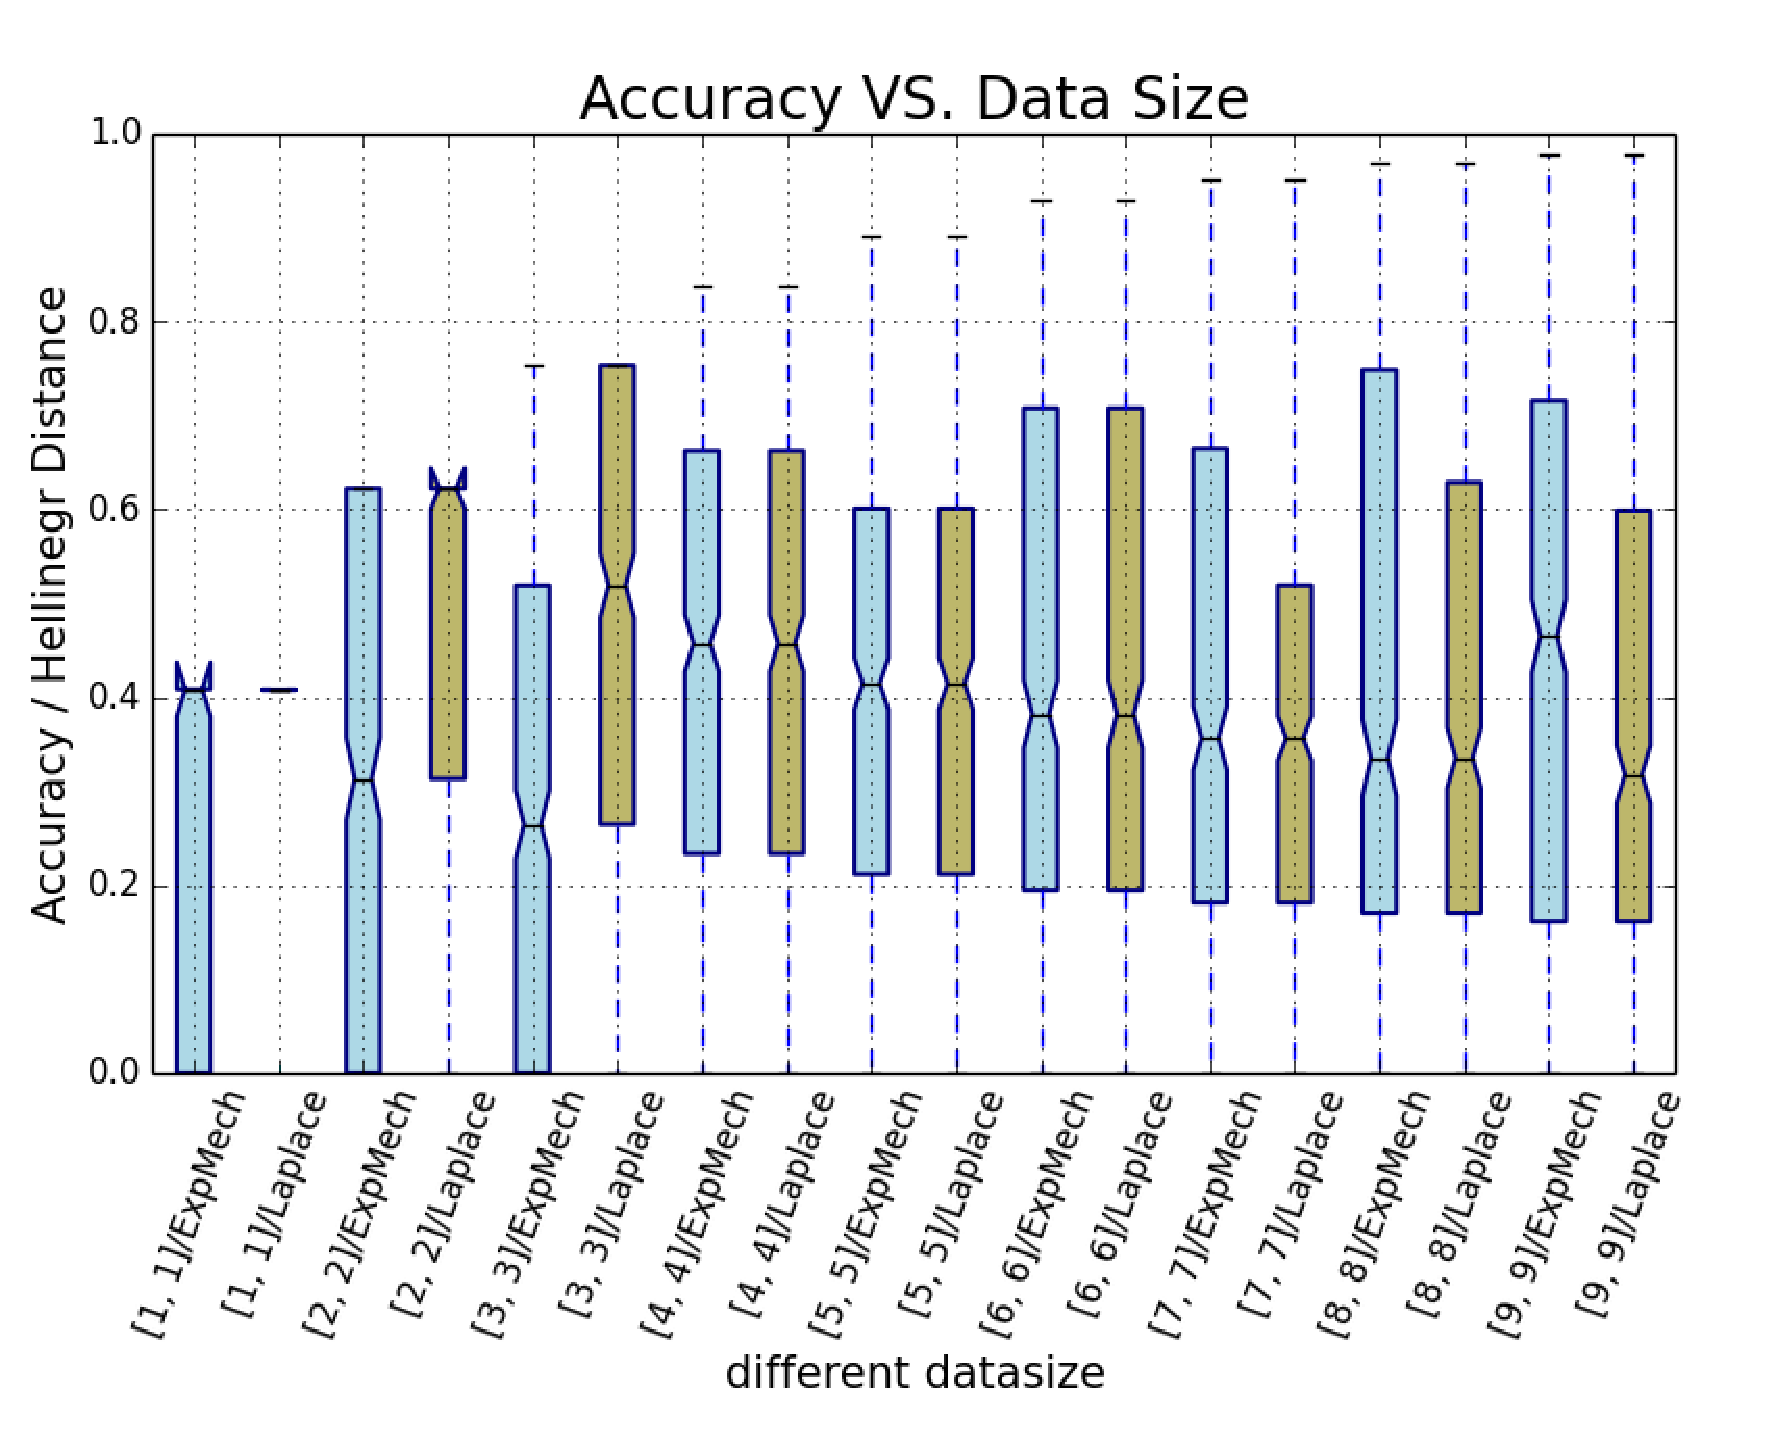
\includegraphics[width=0.3\textwidth]{accuracy_vs_datasize_1_1.eps}}
  \subfigure[three dimensions with $\dirichlet (1,1,1)$ prior distribution]{
    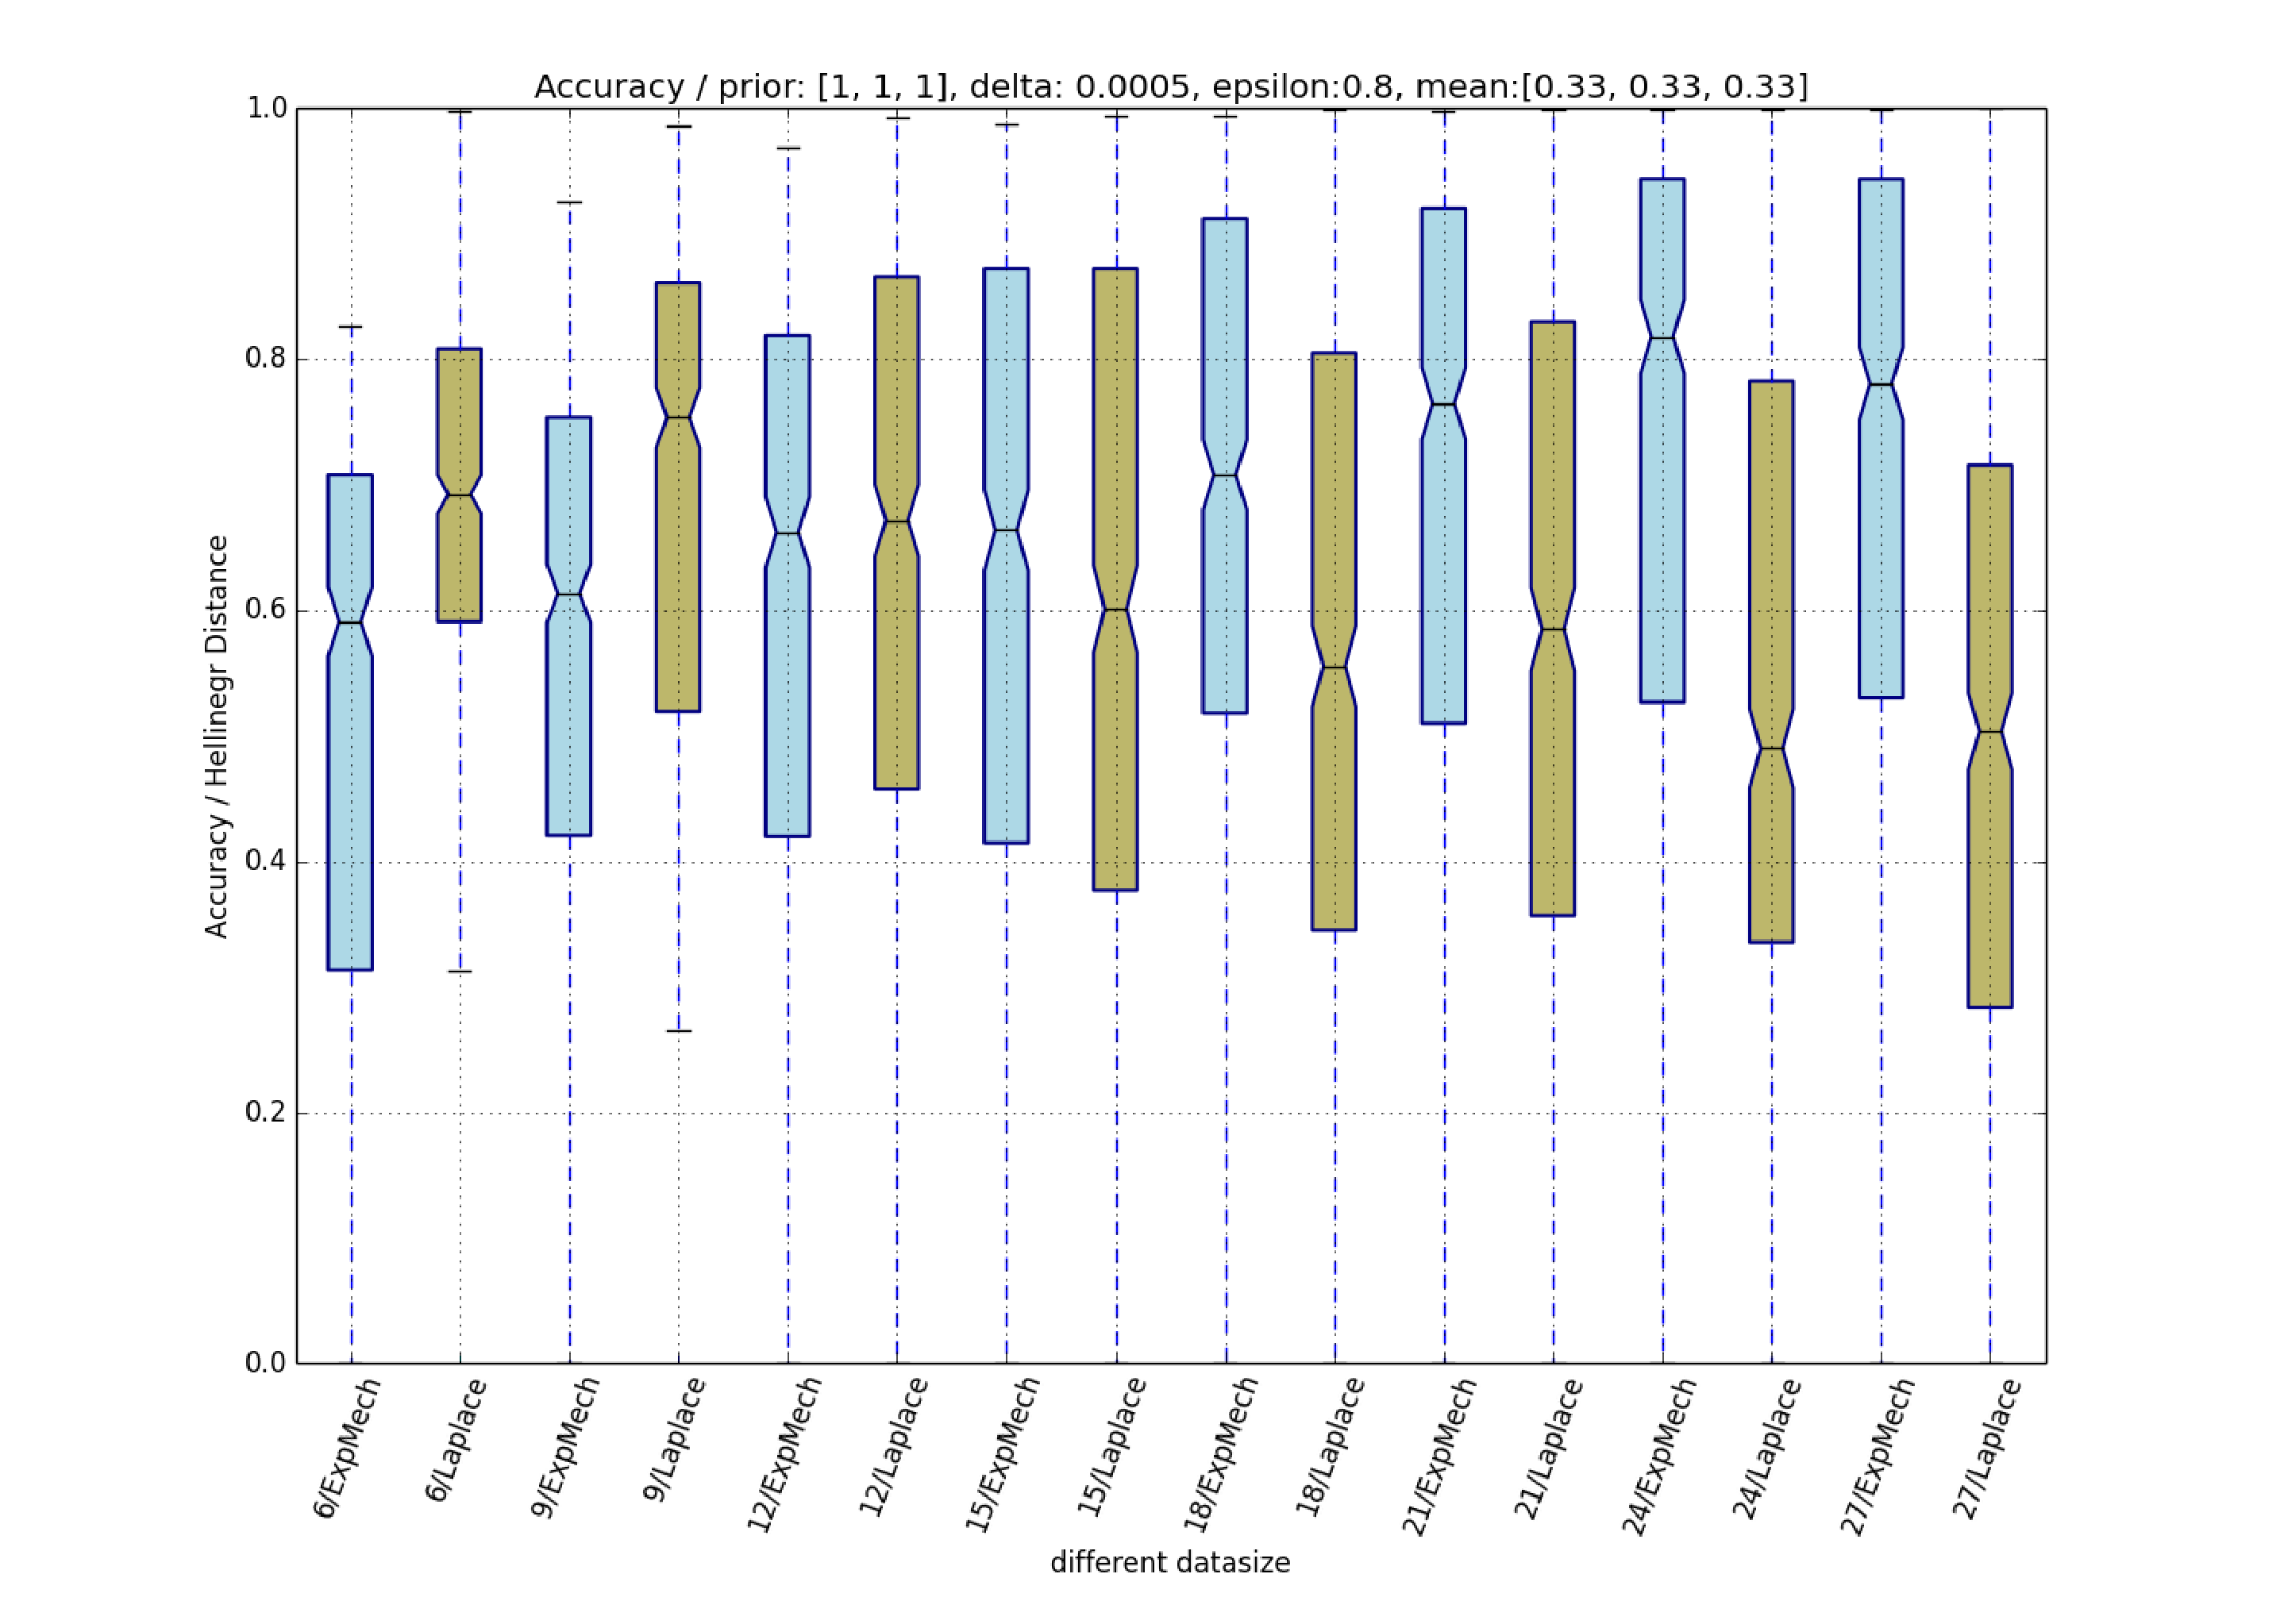
\includegraphics[width=0.3\textwidth]{accuracy_vs_datasize_1_1_1.eps}} 
\caption{Accuracy measurement based on Hellinger distance wrt. different datasizes. Settings: observed data are uniformly distributed, $\epsilon = 0.8$ and $\delta = 0.00000001$}
\label{fig_vs_datasize}
\end{center}
\end{figure}

In Fig. \ref{fig_vs_datasize}, both of the two plots show that when data size go larger, accuracy of our exponential mechanism are decreasing. In Fig. \ref{fig_vs_datasize}(a), when the data size is smaller than 12, we can beta Laplace mechanism but fail when data size larger than or equal to 12. Same as in Fig. \ref{fig_vs_datasize}(b), we can beat Laplace mechanism when data size is smaller than 15 and fail otherwise.

\subsubsection{Accuracy Evaluation wrt. Dimensions}
\label{subsubsec_vs_dimension}


\begin{figure}[ht]
\centering
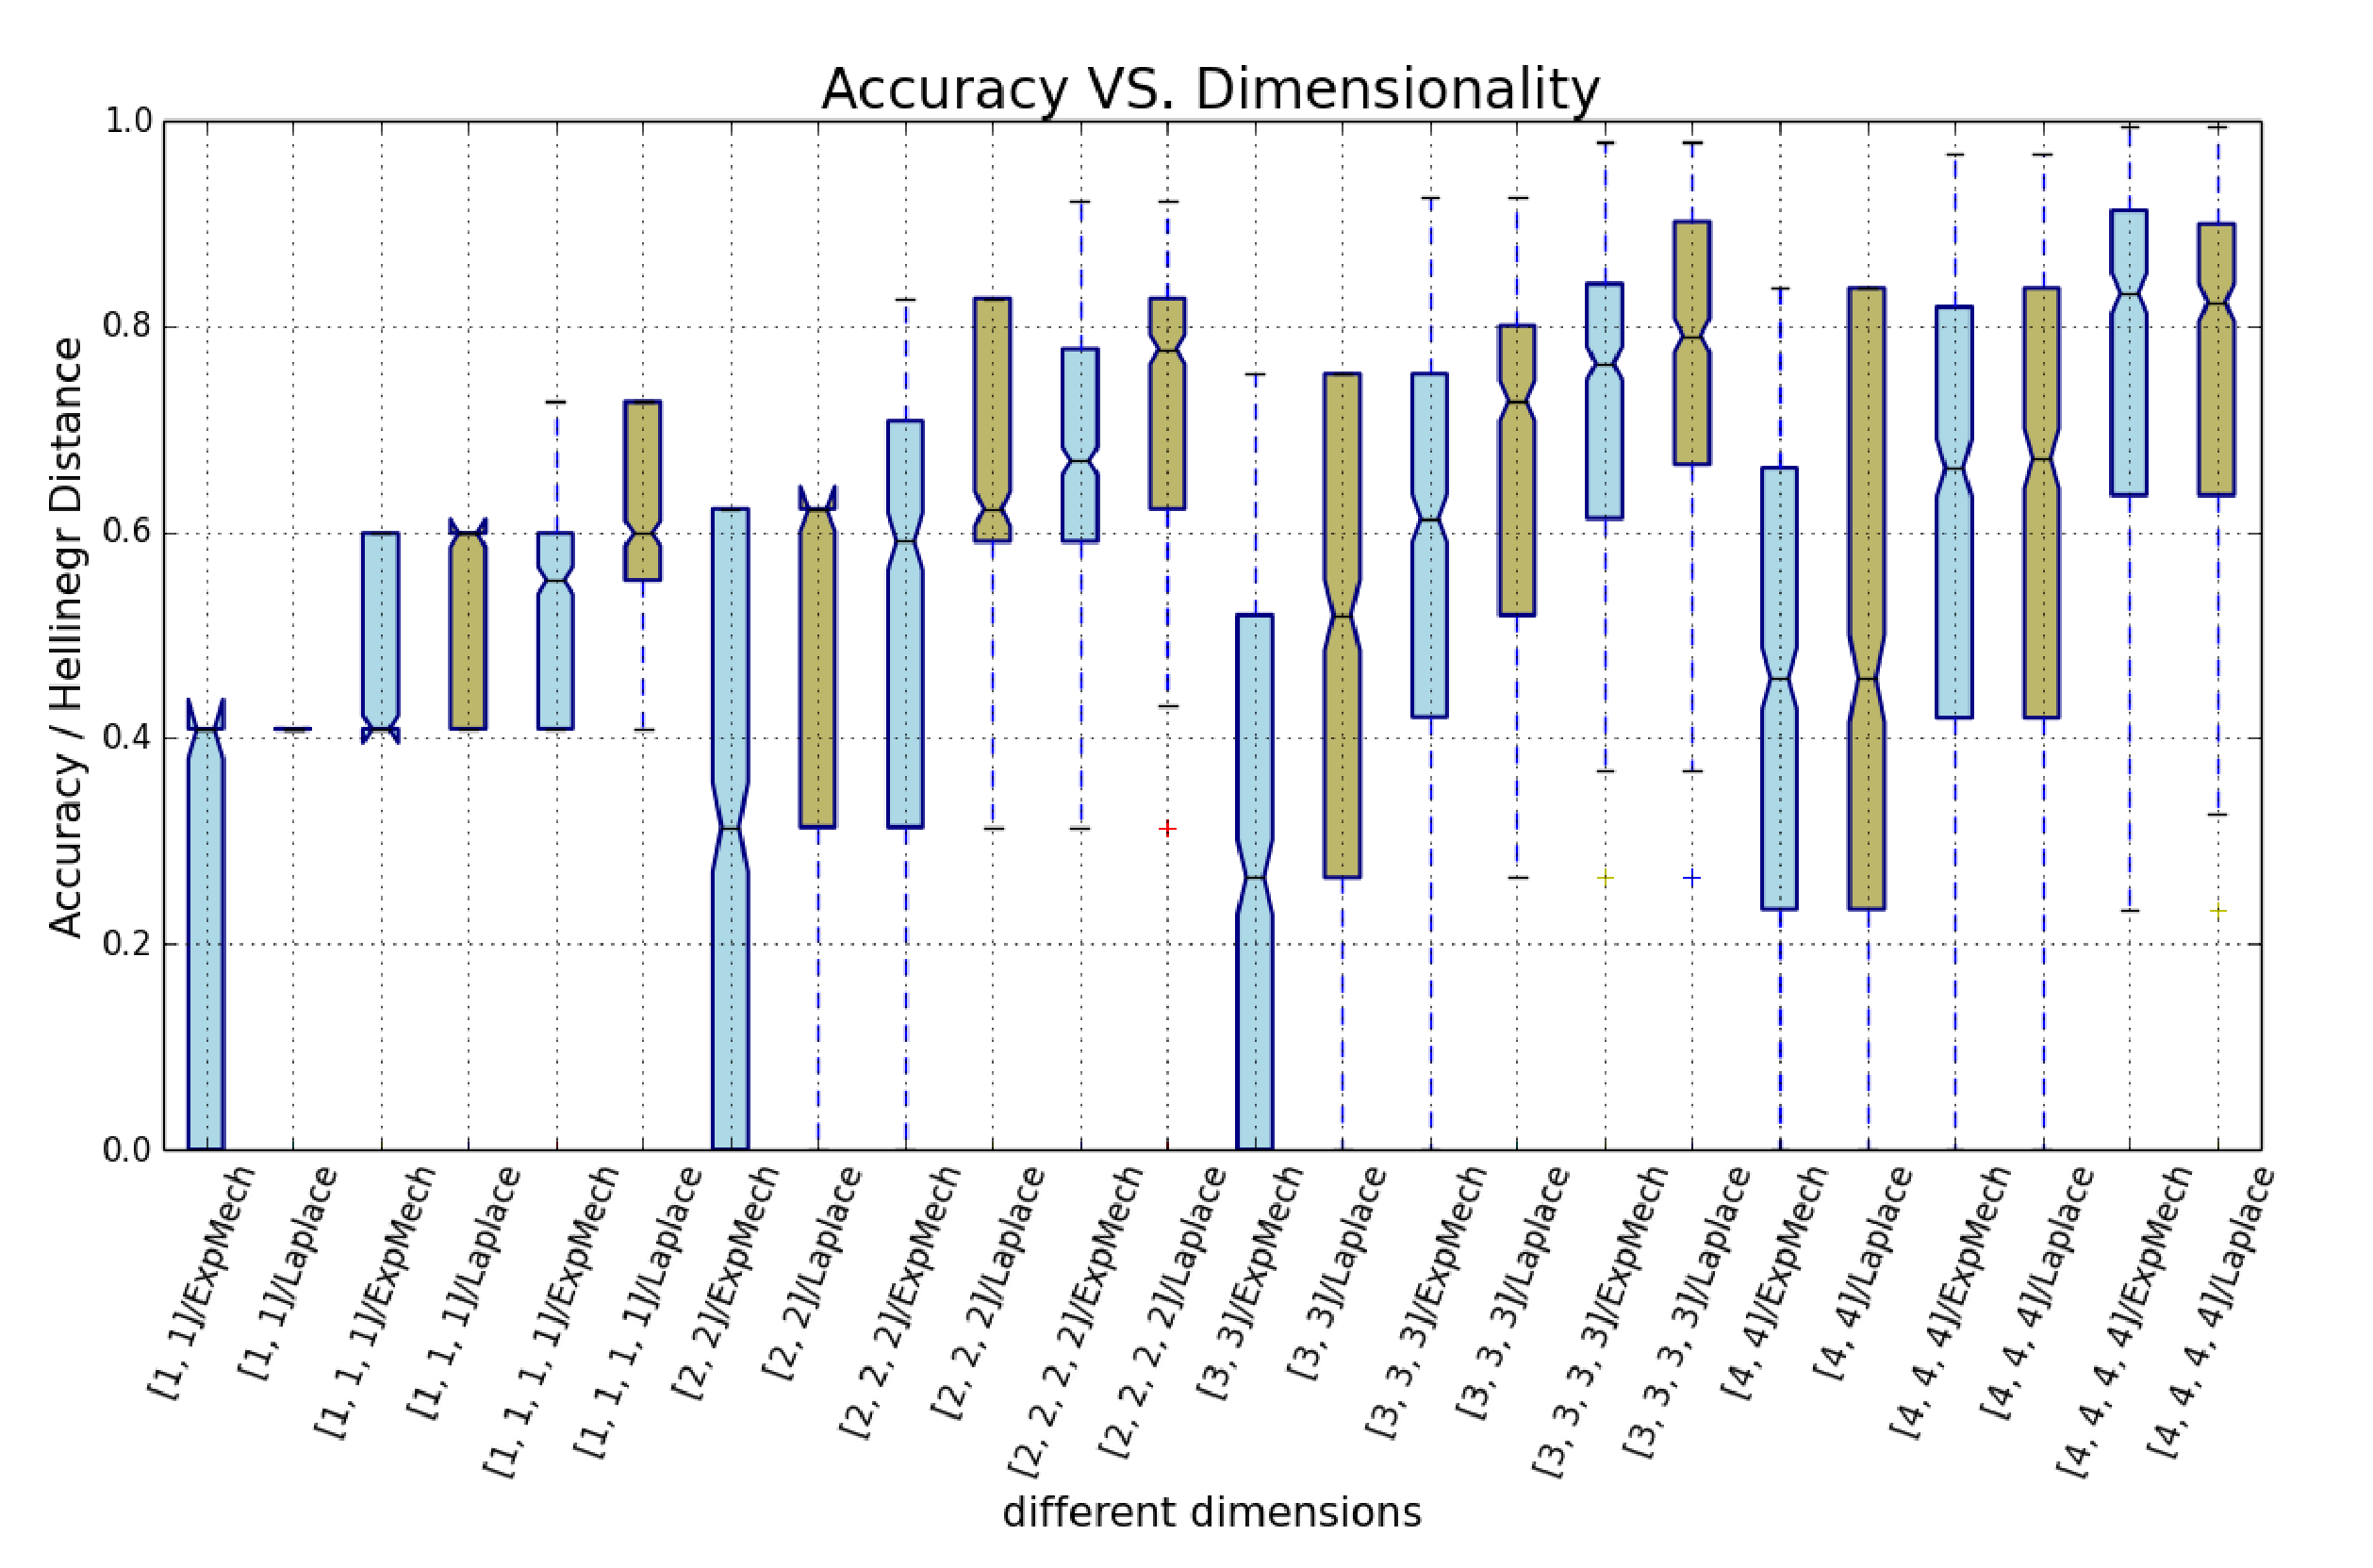
\includegraphics[width=0.45\textwidth]{accuracy_vs_dimension.eps}
\caption{Accuracy measurement based on Hellinger distance wrt. different dimensions and data size. Settings: observed data are uniformly distributed, $\epsilon = 0.8$ and $\delta = 0.00000001$, prior distributions are all $1$ in every dimension}
\label{fig_vs_dimension}
\end{figure}

In Fig. \ref{fig_vs_dimension}, x-axis are observed data sets of different size and dimensions. The plot shows that dimensions have similar influence on our exponential mechanism and the Laplace mechanism. Accuracy of two mechanisms both decrease when dimensions go larger. We will be beat by Laplace mechanism when data size increase but will not be affected when dimensions increase. In other words, dimension has little influence on whether we will beat Laplace mechanism.


\subsubsection{Accuracy Evaluation wrt. Data variance}
\label{subsubsec_vs_variance}

\begin{figure}[ht]
\centering
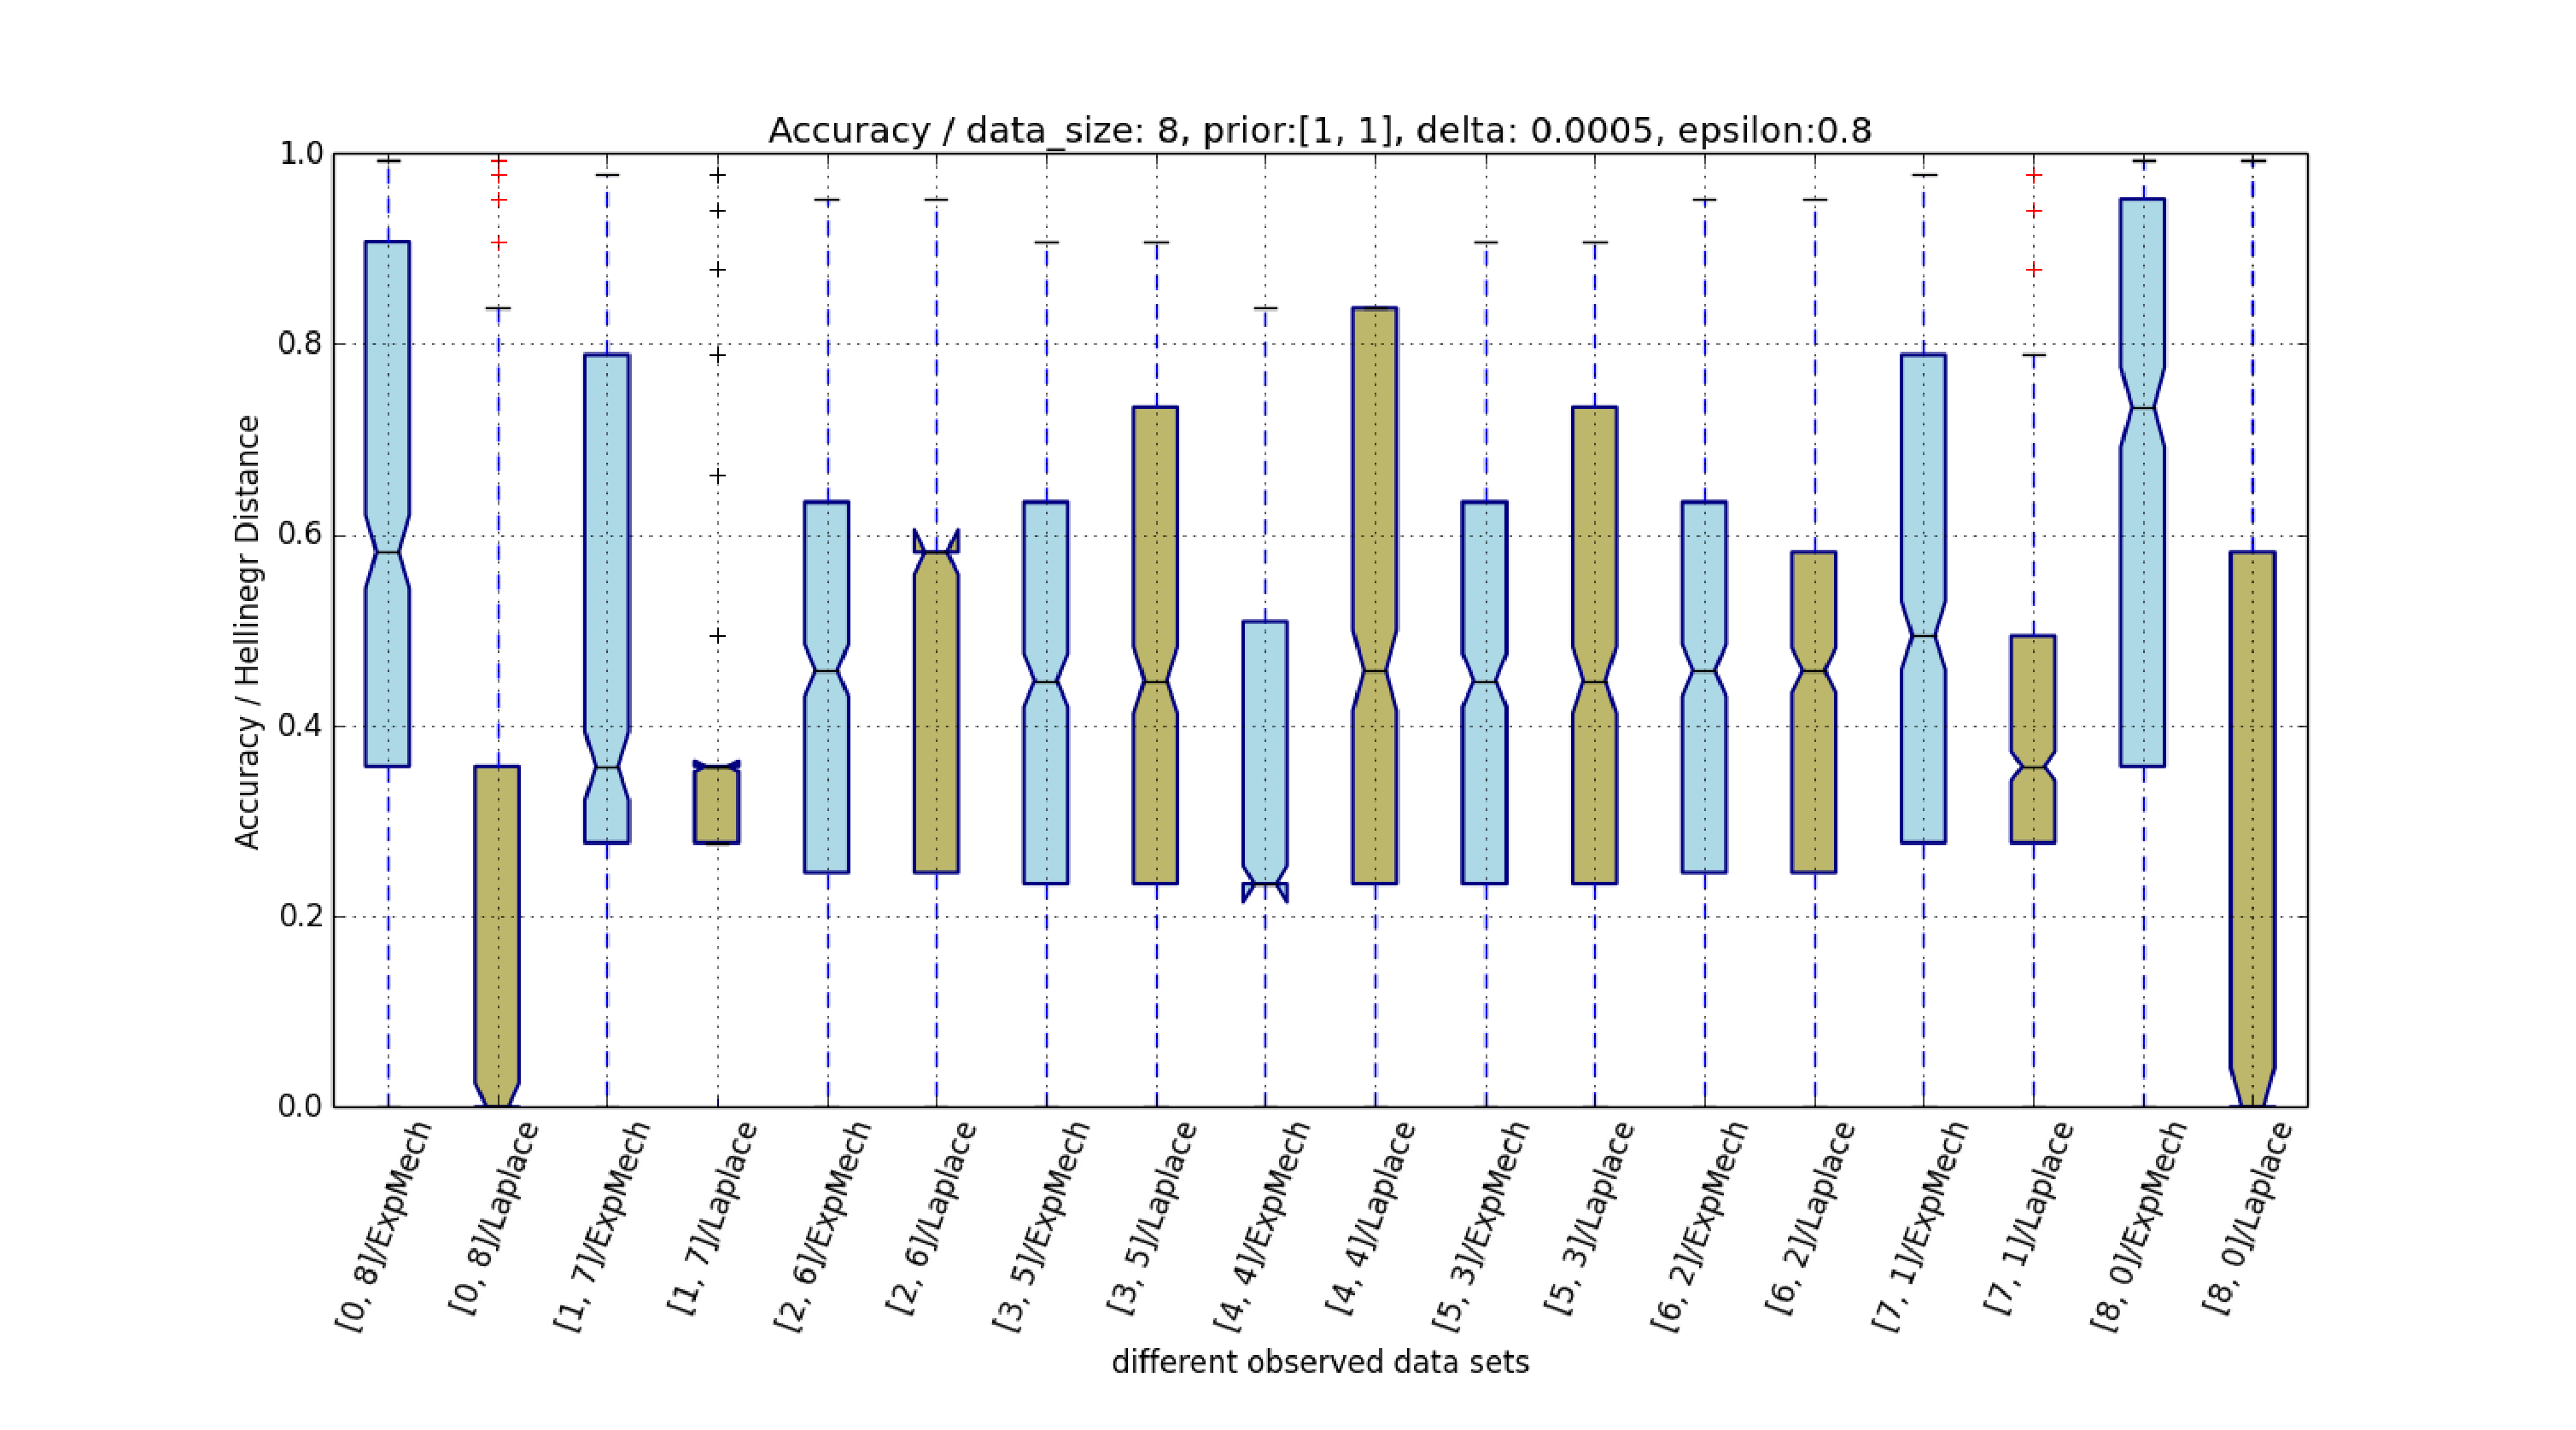
\includegraphics[width=0.45\textwidth]{accuracy_vs_mean_1_1.eps}
\caption{Accuracy measurement based on Hellinger distance wrt. different data variance. Settings: $\epsilon = 0.8$ and $\delta = 0.00000001$, prior distributions are all $1$ in every dimension}
\label{fig_vs_variance}
\end{figure}

In Fig. \ref{fig_vs_variance}, x-axis are observed data sets of different variances (or means). We study this variable under two-dimension $\betad$ distribution in order to be concise. It shows that our mechanism's accuracy is better when data variance go smaller, meanwhile Laplace mechanism go worse. We will beat Laplace mechanism when observed data are more uniformly.



\subsubsection{Accuracy Evaluation wrt. Prior Distribution}
\label{subsubsec_vs_prior}

\begin{figure}[ht]
\centering
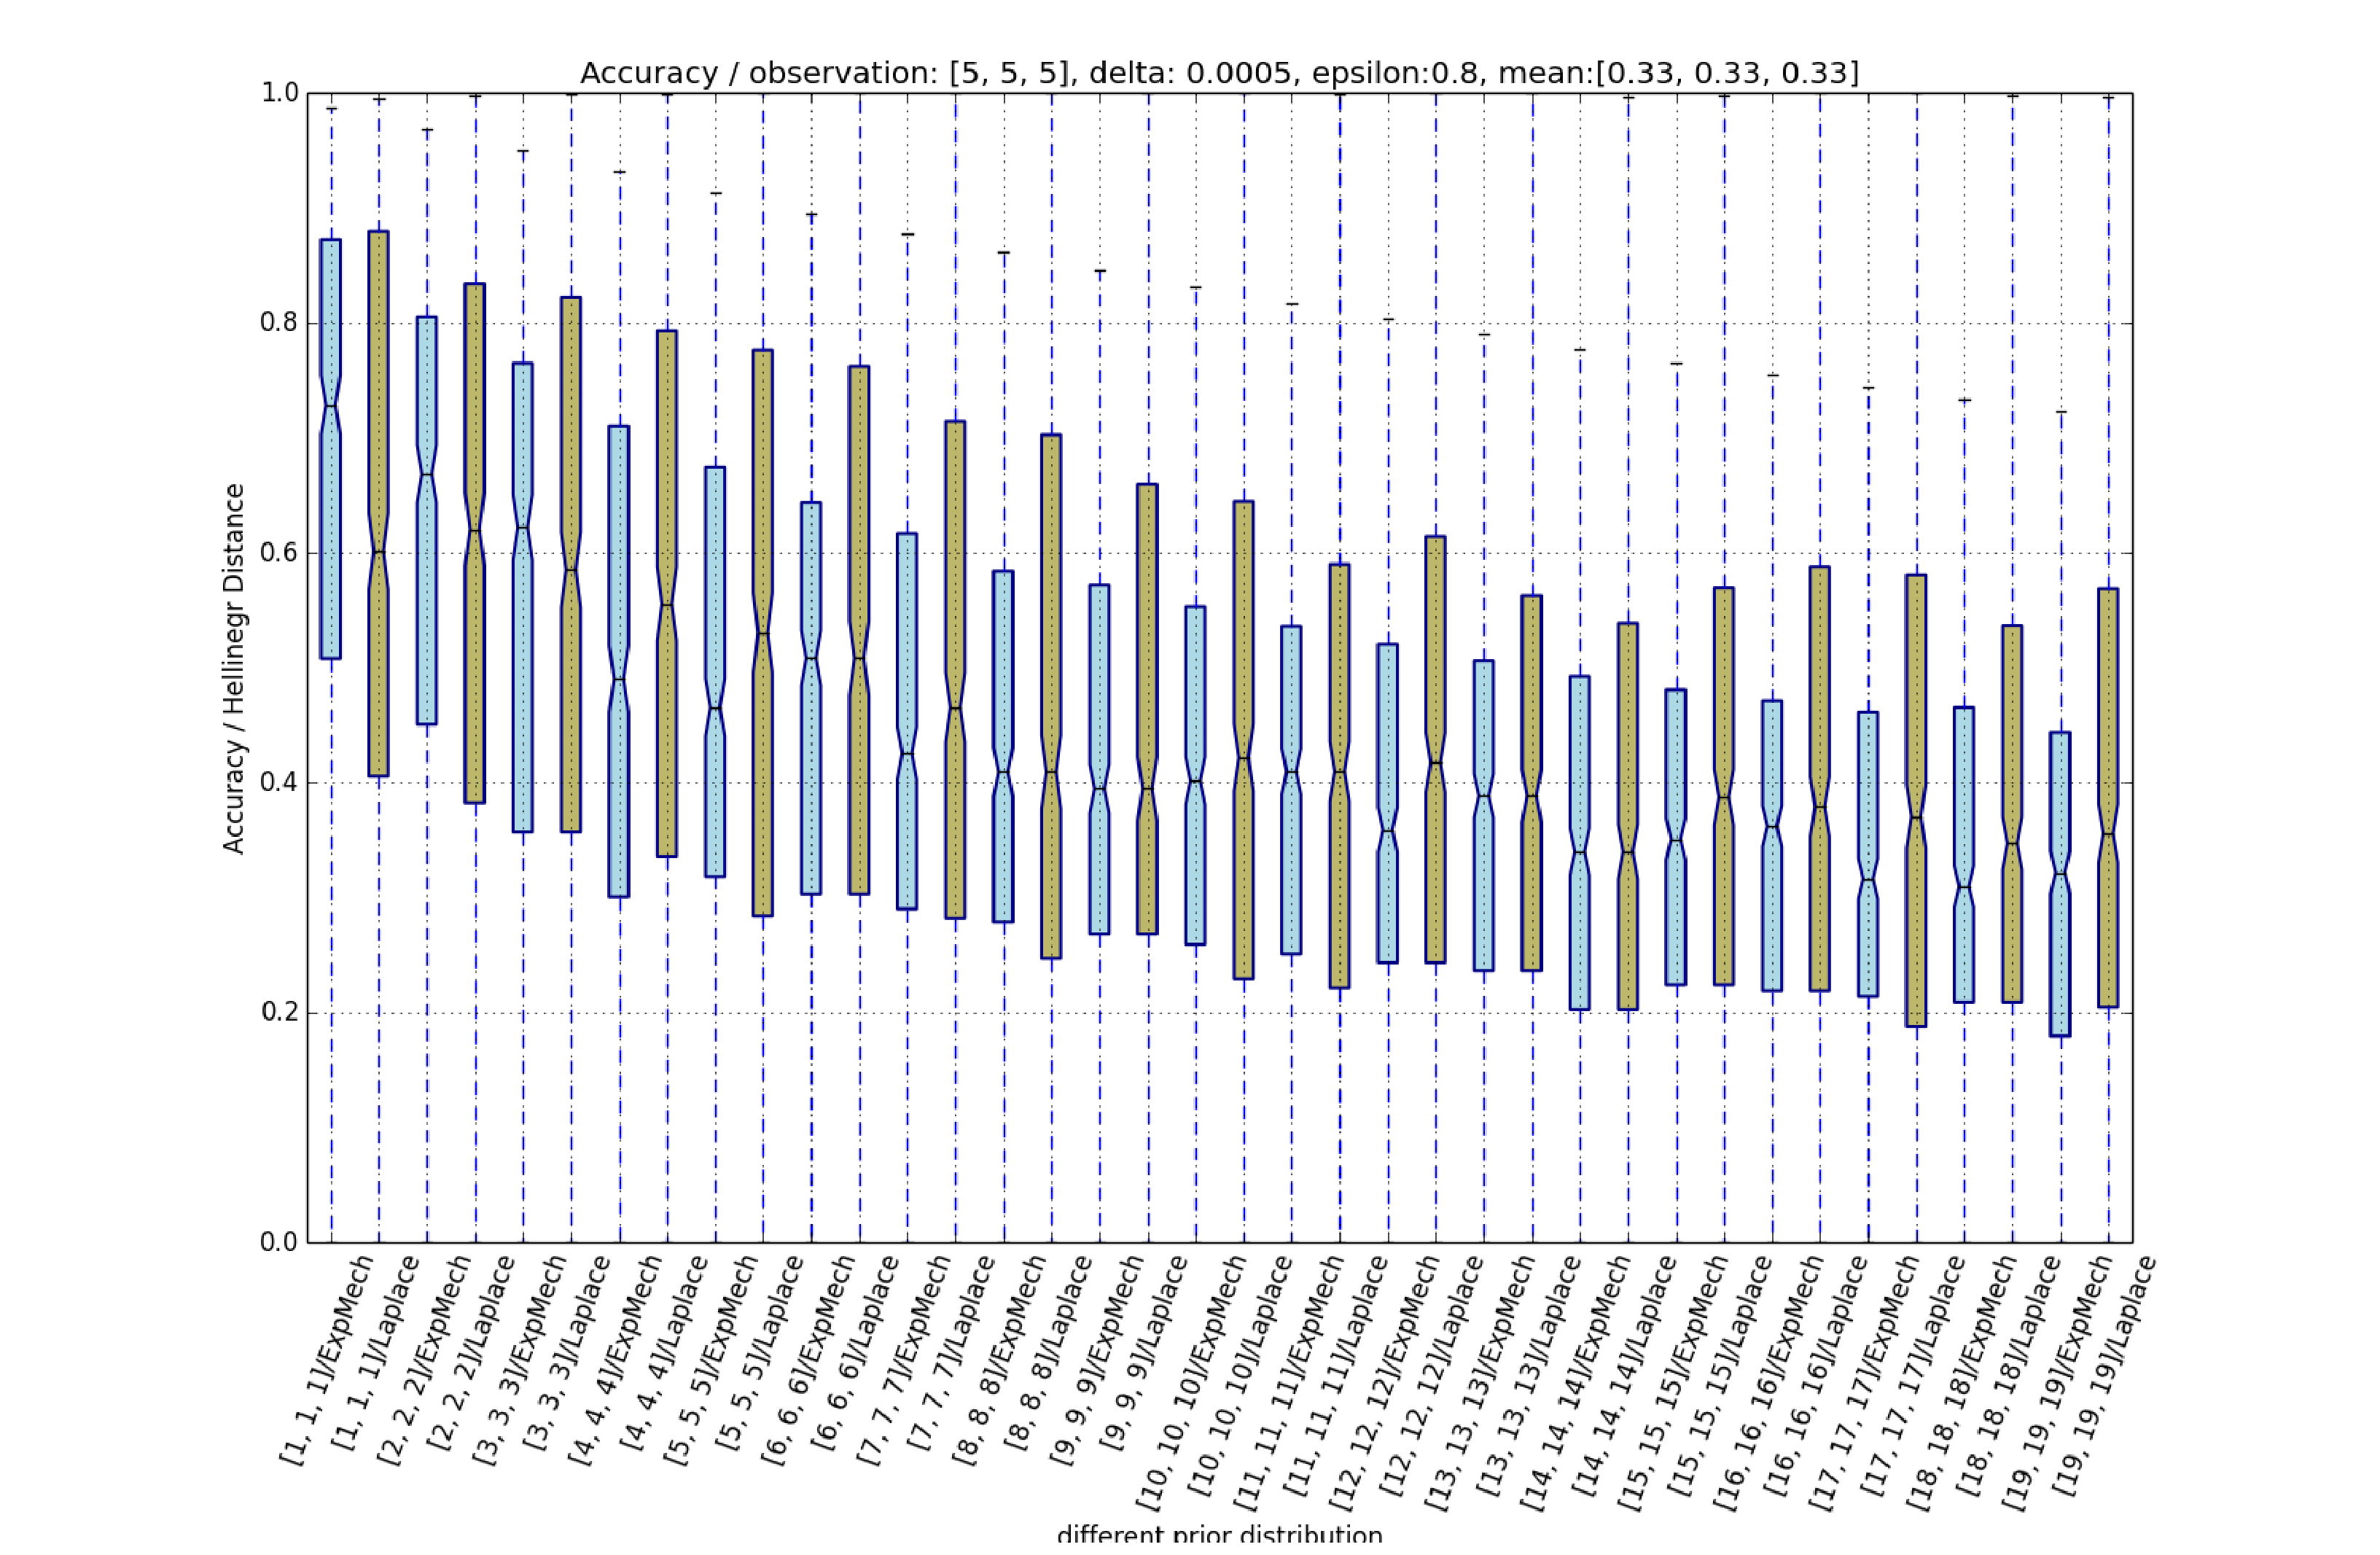
\includegraphics[width=0.45\textwidth]{accuracy_vs_prior_5_5_5.eps}
\caption{Accuracy measurement based on Hellinger distance wrt. different prior distribution. Settings: $\epsilon = 0.8$ and $\delta = 0.00000001$, observed data set is: $[5,5,5]$}
\label{fig_vs_prior}
\end{figure}

In Fig. \ref{fig_vs_prior}, we study this variable under setting that observed data set is $[5,5,5]$ because in Fig. \ref{fig_vs_datasize} Laplace mechanism beat us when data size is 15 and uniformly distributed. The plot shows that in the beginning we cannot beat Laplace but when prior distribution grow larger, we perform better and better and beat Laplace mechanism finally.



% \subsubsection{Accuracy Evaluation wrt. Prior Distribution and Data Variance}
% \label{subsubsec_vs_prior_variance}

% \begin{figure}[ht]
% \centering
% 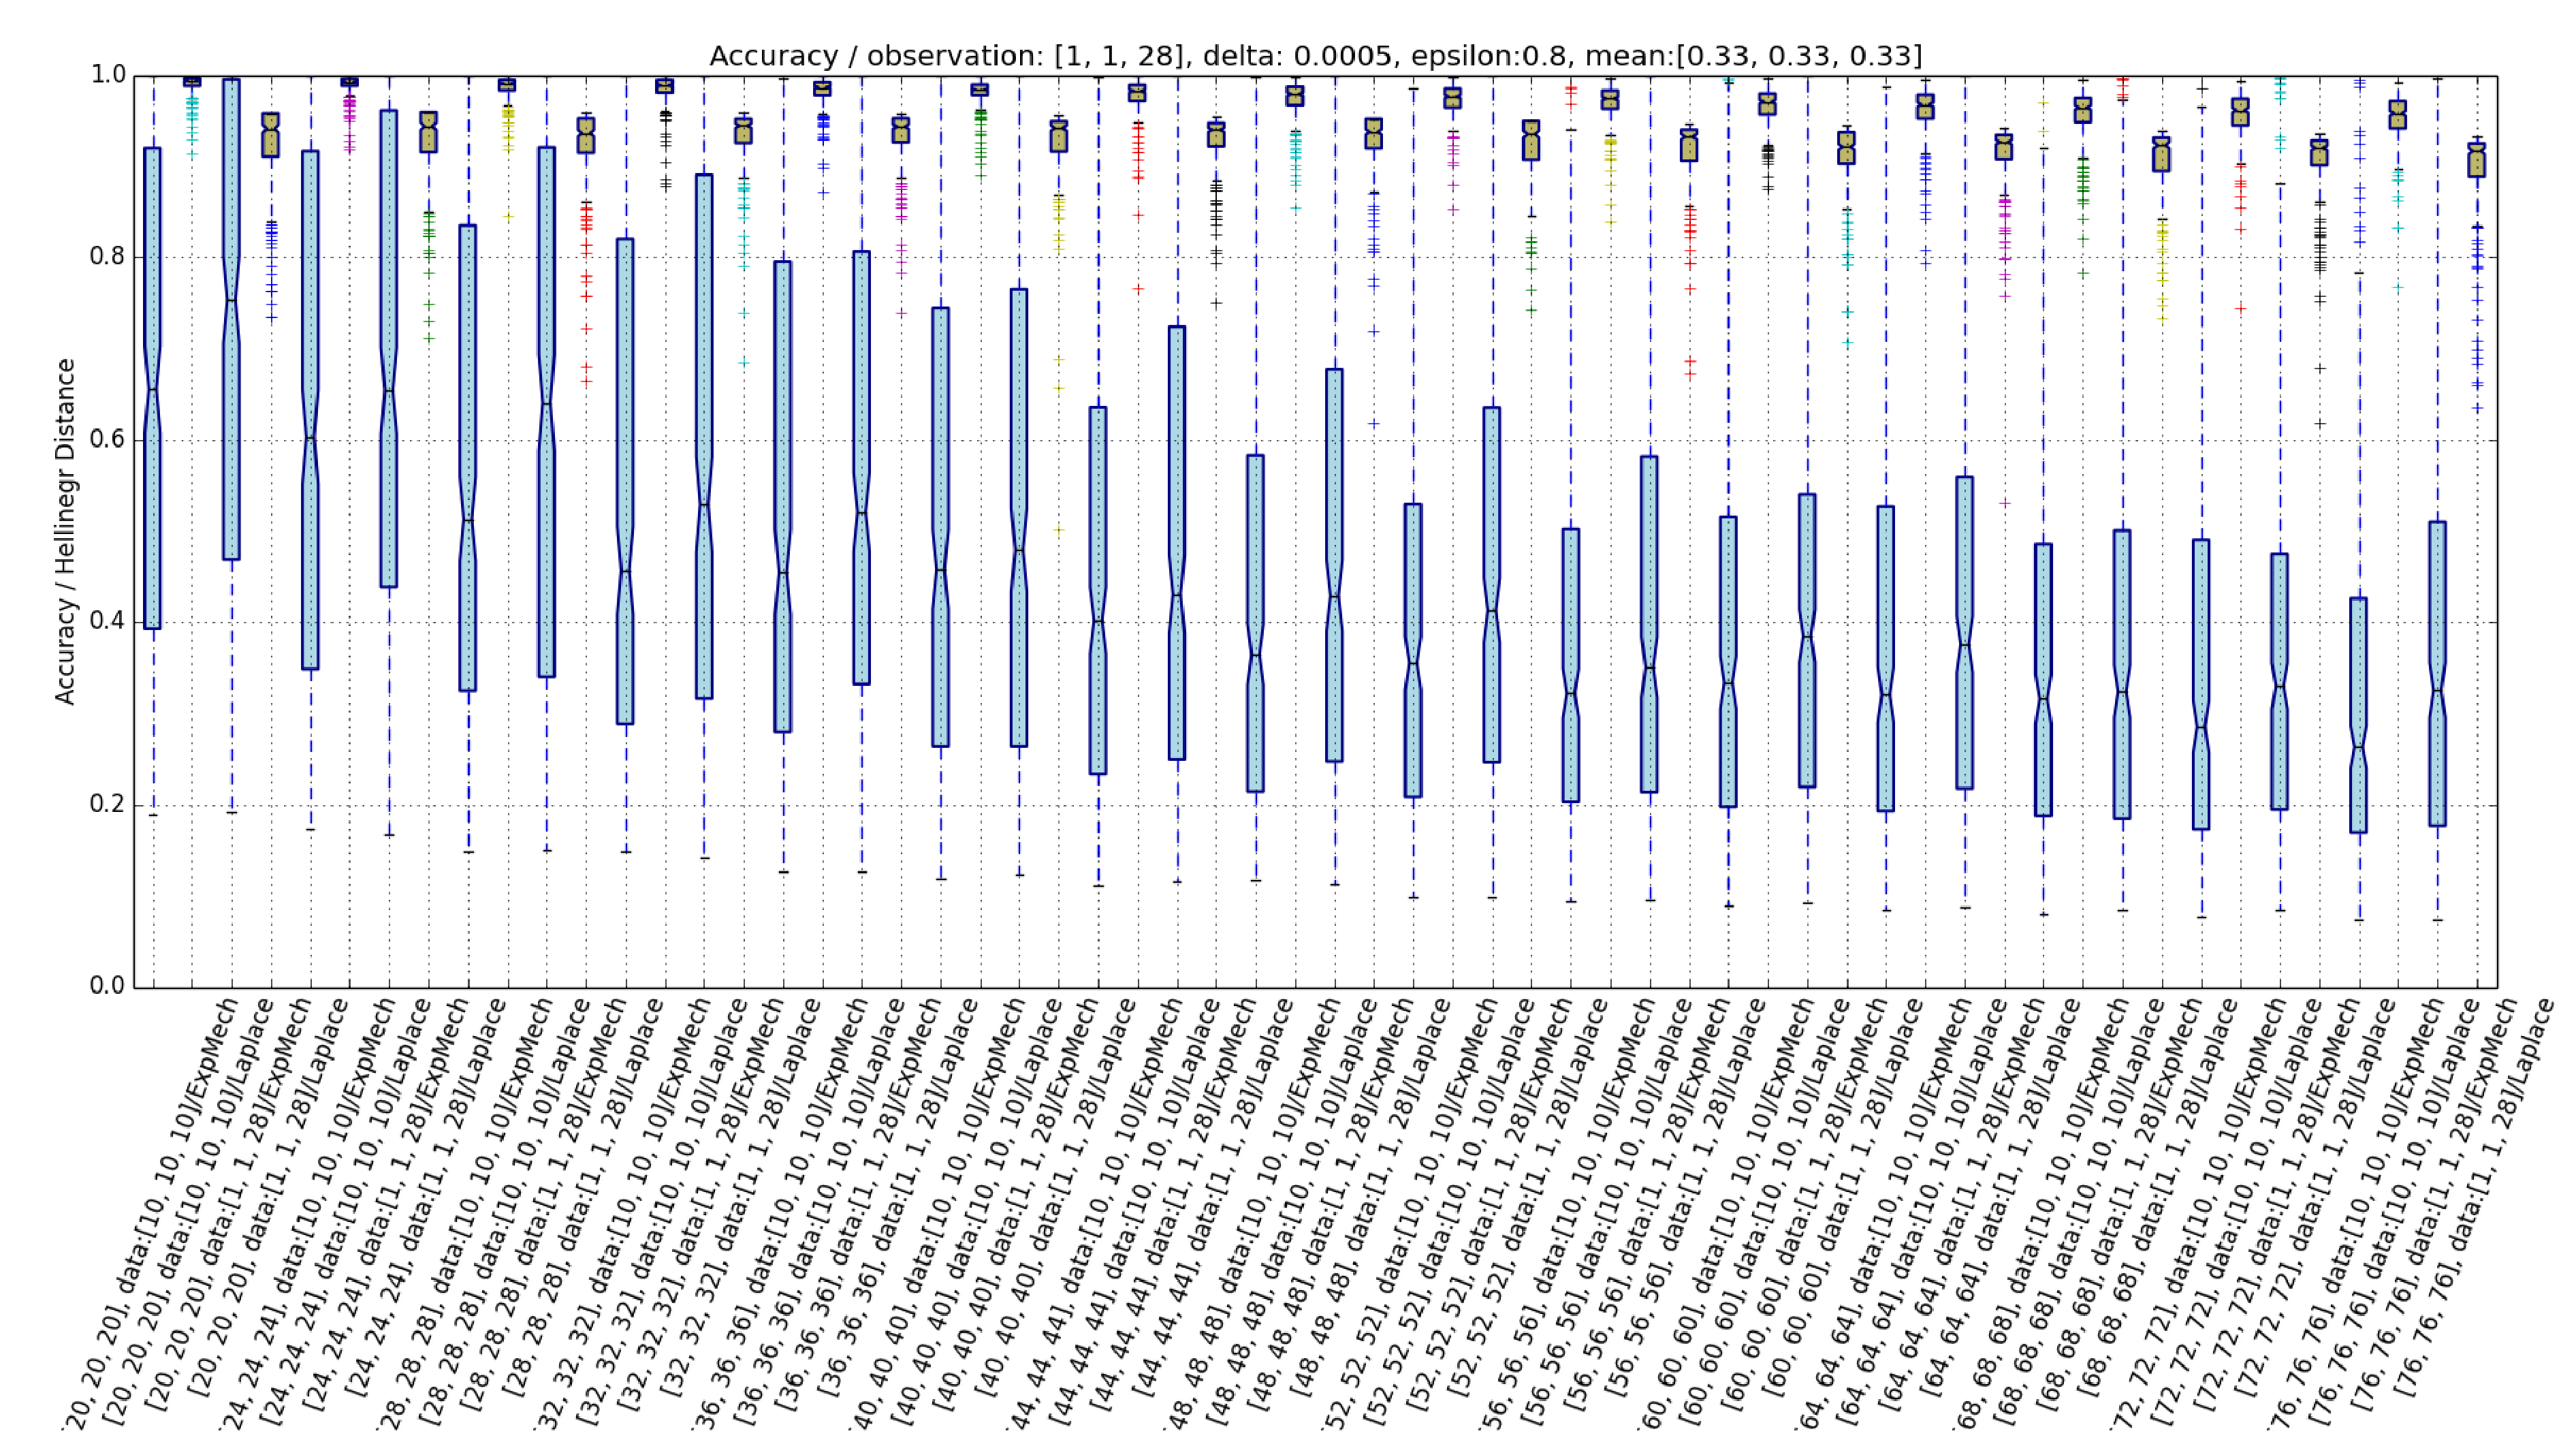
\includegraphics[width=0.45\textwidth]{Accuracy_VS_Prior_mean.eps}
% \caption{Accuracy measurement based on Hellinger distance wrt. different prior distribution and data variances. Settings: $\epsilon = 0.8$ and $\delta = 0.00000001$, observed data sets are $[10,10,10]$ and $[1,1,28]$ and prior distributions are range from $[20,20,20]$ to $[76,76,76]$}
% \label{fig_vs_prior_variance}
% \end{figure}

% Here, we change the prior distribution and data variance in the same time. As shown in Fig. \ref{fig_vs_prior_variance}, our exponential mechanism do better in uniform data set than in edging data set while Laplace mechanism on the contrary. Moreover, our mechanism is improving continuously and significantly as prior distribution increasing while Laplace mechanism isn't.


\section{Conclusions}
We can obtain some preliminary conclusions: 
\begin{enumerate}
	\item We can beat Laplace mechanism when data size is small.
	\item We will beat Laplace mechanism when observed data are more uniformly.
  \item When prior distribution grow larger, we perform better and better and beat Laplace mechanism finally.
\end{enumerate} 

In consequence, we have a better accuracy in small data size, in larger prior and in uniformly data.



\bibliographystyle{ACM-Reference-Format}
\bibliography{bayesian.bib}

\end{document}
 % TODO: replace with your brilliant paper!
% 
%packages
\usepackage{natbib}
\usepackage{amsmath}
\usepackage{amsthm}
\usepackage{mathtools}
\usepackage{mdframed}
\usepackage{subfigure}
\usepackage{booktabs}
% \usepackage{hyperref}
\usepackage{subfigure}
\usepackage{siunitx} % Provides the \SI{}{} and \si{} command for typesetting SI units
\usepackage{graphicx} % Required for the inclusion of images
% \usepackage{natbib} % Required to change bibliography style to APA
\usepackage{datetime}
\usepackage{lscape}
\usepackage{algorithm}
\usepackage{algorithmic}
\usepackage{xspace}
\usepackage[english]{babel} % English language/hyphenation
\usepackage{proof}
\usepackage{booktabs} % Top and bottom rules for tables
\usepackage[colorlinks, allcolors = blue,]{hyperref}
\usepackage{accents}
\usepackage{amsfonts}
\usepackage{stmaryrd}
\usepackage{amsmath,amsthm,amssymb,latexsym} 
\usepackage{microtype}
\usepackage{graphicx}
\usepackage{subfigure}
\usepackage{booktabs} % for professional tables
\usepackage{hyperref}
\usepackage{icml2019}
\usepackage{lipsum}

\usepackage{authblk}


%new commands
\newcommand{\theHalgorithm}{\arabic{algorithm}}
\newtheorem{definition}{Definition}
\usepackage{cancel}
\usepackage[normalem]{ulem}
\newcommand{\dataobs}{\textbf{x}}
\newcommand{\adj}[2]{\textbf{adj}(#1,#2)}
\newcommand{\candidateset}{\mathcal{R}_{\textup{post}}}
\newcommand{\bprior}{\boldsymbol{\beta}_{\textup{prior}}}
\newcommand{\bysinfer}{\mathsf{Infer}}
\newcommand{\betad}{\mathsf{Beta}}
\newcommand{\betaf}{\textup{B}}
\newcommand{\mbetaf}{\boldsymbol{\textup{B}}}
\newcommand{\vtheta}{\boldsymbol{\theta}}
\newcommand{\valpha}{\boldsymbol{\alpha}}
\newcommand{\vbeta}{\boldsymbol{\beta}}
\newcommand{\lapmech}{\mathsf{LSDim}}
\newcommand{\ilapmech}{\mathsf{LSHist}}
\newcommand{\binomial}[2]{\mathsf{Bin}(#1, #2)}
\newcommand{\multinomial}[2]{\mathsf{Mult}(#1, #2)}
\newcommand{\expmech}{\mathsf{EHD}}
\newcommand{\hexpmech}{\mathsf{EHDS}}
\newcommand{\lexpmech}{\mathsf{EHDL}}
\newcommand{\hexpmechd}{\mathsf{expMech}^{D}_{\hellinger}}
\newcommand{\privinfer}{\mathsf{PrivInfer}}
\newcommand{\hlg}{\mathsf{H}}
\newcommand{\dirichlet}[1]{\mathsf{Dir}(#1)}
\newcommand{\alphas}{\boldsymbol{\alpha}}
\newcommand{\xis}{\boldsymbol{\xi}}
\newcommand{\iverson}[1]{[#1]}
\newcommand{\datauni}{\mathcal{X}}
\newcommand{\hellinger}{\mathcal{H}}
\newcommand{\ux}[1]{u(\textbf{x}, {#1})}
\newcommand{\uxadj}[1]{u(\textbf{x}', {#1})}
\newcommand{\cardinality}[2]{\mathcal{C}^{#1}_{#2}}
\newcommand{\range}{\mathcal{O}}
\newcommand{\nomalizer}[1]{\sum\limits_{r'\in \mathcal{R}_{\textup{post}}} \exp \big(\frac{-\epsilon\cdot \mathcal{H} (\mathsf{BI}(#1),r')}{4 \cdot S(#1)}\big)}

\newcommand{\unomalizer}[1]{\sum\limits_{r'\in \mathcal{R}_{\textup{post}}} \exp \big(\frac{-\epsilon\cdot u(#1, r')}{4 \cdot S(#1)}\big)}


\newcommand{\hexpmechPr}[2]{\underset{z \thicksim \hexpmech(#1)}{\Pr}\left[ #2 \right]}
\newcommand{\lapmechPr}[2]{\underset{z \thicksim \lapmech(#1)}{\Pr}\left[ #2 \right]}

\newcommand{\ilapmechPr}[2]{\underset{
{z \thicksim \ilapmech(#1)}
}{\Pr}\left[ #2 \right]}

\newtheorem{thm}{Theorem}[section]

\newtheorem{lem}{Lemma}[section]

\newtheorem{assert}{Assertion}[lem]
\newcommand{\lap}[2]{\mathsf{Lap}(#1, #2)}
\newcommand{\todo}[1]{{\footnotesize \color{red}\textbf{[[ #1 ]]}}}

\section{Bayesian Inference Background}
Given a prior belief $\Pr(\theta)$ on some parameter $\theta$,
and given an observation $\dataobs$,
the posterior distribution on $\theta$ given $\dataobs$ is computed as:
\[
  \Pr(\theta | \dataobs) = \frac{Pr(\dataobs | \theta) \cdot \Pr(\xis)}{\Pr(\dataobs)}
\]
where the expression  $\Pr(\dataobs | \theta)$ denotes the \emph{likelihood} of $\theta$ when
\dataobs~ is observed. Since we consider \dataobs to be fixed the likelihood is a function of $\theta$.
For the same reason $\Pr(\dataobs)$ is a constant independent of $\theta$.
Usually in statistics the prior distribution $\Pr(\theta)$ is chosen so that it represents
the initial belief on $\theta$. That is, when no data has been observed. In practice though,
prior distributions and likelihood functions are usually chosen so that the posterior
belongs to the same \emph{family} of distributions. In this case we say that the prior
is conjugate of the likelihood function. Using conjugate priors simplify calculcations and allows
for inference to be performed in a recursive fashion over the data.
In this work we will consider a specific instance of Bayesian inference and one of its generalizations.
Specifically, we will consider the situation where $\theta$ represents the parameter --informally called \emph{bias})--
of a Bernoulli distributed random variable, and its immediate generalization where the parameter $\vtheta$ represents
the the vector of parameters of a categorical distributed random variable.
In the former case the prior distribution over $\theta\in [0,1]$ is going to be a beta distribution, $\betad(\alpha, \beta)$, with parameters
$\alpha,\beta\in\mathbb{R}^{+}$, and with p.d.f:
\[
  \Pr(\theta)\equiv \frac{\theta^{\alpha} (1- \theta)^{\beta}}{\betaf(\alpha,\beta)}
\]
where $\betaf(\cdot,\cdot)$ is the beta function.
The data $\dataobs$ will be a sequence of $n\in\mathbb{N}$ 0/1 values, that is $\dataobs=\ll x_1,\dots x_n \gg, x_i\in\{0,1\}$, and the likelihood function is:
\[
  \Pr(\dataobs | \theta)\equiv \theta^{a}(1-\theta)^{n-a}
\]
where $a=\displaystyle\sum_{i=1}^{n}\mathrm{x_i}$.
From this it can easily be derived that the posterior distribution is:
\[
  \Pr(\theta|\dataobs)=\betad(\alpha+a,\beta+n-a)
\]
In the latter case the prior distribution over $\vtheta\in [0,1]^{k}$ is given by a Dirichelet distribution, $\dirichlet(\vtheta)$, for $k\in\mathbf{N}$,
and $\valpha\in(\mathbf{R^{+}})^{k}$, with p.d.f:
\[
  \Pr(\vtheta)\equiv\frac{1}{\mbetaf(\valpha)}\cdot \displaystyle\prod_{i=1}^{k}{\theta_i^{\alpha_i-1}}
\]
where $\mbetaf(\cdot)$ is the generealised beta function.
The data $\dataobs$ will be a sequence of $n\in\mathbb{N}$ values coming from a universe $\datauni$, such that $\mid\datauni \mid=k$.
The likelihood function will be:
\[
  \Pr(\dataobs|\vtheta)\equiv \displaystyle\prod_{a\in\datauni}\alpha_{a}^{z_a}
\todo{to check}\]
where $z_a=\displaystyle\sum_{i=1}^{n}\iverson{x_i=a}$, where in $\iverson{\cdot}$ we use
Iverson bracket notation. The posterior distribution over $\vtheta$ turns out to be
\[
  \Pr(\vtheta|\dataobs)=\todo{to type down}\dirichlet(\vtheta+...)
\]
\section{Problem Statement}
% When we try
% to make this distribution public, sensitive information of the data
% based on which the posterior drew from can be compromised. So, it is
% important to protect this posterior distribution. When our protection
% objective is a distribution rather than a numeric value or vector, it
% would be better to measure the accuracy by distance over
% distributions, for instance, Hellinger distance, than by numeric
% metrics like $\ell_1$-norm.
This work will show that the same mechanism can
perform differently when its accuracy is computed w.r.t to a metric
over probability measures (e.g total variation distance, or Hellinger distance)
from when the metric (e.g. $\ell_1$-norm) is over the parameters.  
\section{Technical Problem Statement}
\label{sec_bayesInfer}
The posterior belief about parameters $\xis$ is inferred from the
group of sensitive data. Because it is usually published in form of a
distribution, for example, $\betad(\alpha',\beta'), \cdots,$ itself
can relieve a lot of information about sensitive data. So, the
sensitive information we want to protect here is the posterior belief,
i.e., $Pr(\xis | \dataobs)$, rather than just a sample drew from
it\cite{foulds2016theory}. Then it will be better if we can use a
distance over two distributions to measure the accuracy than a
distance over just parameters or values when we are protecting a
distribution, for instance, Hellinger distance in our paper. When we
measure the accuracy between true posterior and protected posterior
using Hellinger distance, it would be better we can have a protection
mechanism based on Hellinger distance. However, current mechanisms are
mainly based on $l_1$ norm by Laplace mechanism
\cite{zhang2016differential} \cite{xiao2012bayesian}. That's why we
design our exponential mechanism over Hellinger distance to protect
the whole posterior distribution.


\section{Baseline Approach - Laplace Mechanism}
\label{sec_lap}
Based on the posterior results from Bayesian inference, we calculate the Laplace mechanism updates on posterior and get the private results under Laplace mechanism. In the case of $m$ dimension Dirichlet distribution, we will add $(m-1)$ i.i.d. Laplace noises $\{| Lap_1 |, | Lap_2 |, \cdots, | Lap_{m-1} |\}$ to the output, where $Lap_i = floor(Y)$, $Y \sim Lap(\frac{2}{\epsilon})$. The private posterior then will be $\dirichlet(\alpha_1 + n_1 + | Lap_1 |, \alpha_2 + n_2 + | Lap_2 |, \cdots, \alpha_m + n - (Lap_1 + \cdots + Lap_{m-1}))$.

\section{Our Approach - Exponential Mechanism with Smooth Sensitivity}
\label{sec_smoo}

% \subsection{Algorithm Setting up}
We define a new mechanism $\hexpmech(x)$ which is similar to the exponential mechanism where we use $\mathcal{R}$ as the set $\betaset$ of beta distributions with integer parameters summing up to $n+2$, as scoring function we use the Hellinger distance from $\bysinfer(x)$, i.e. $\hlg(\bysinfer(x),-)$, and we calibrate the noise to the smooth sensitivity~\cite{nissim2007smooth}. The only difference is in the sensitivity part, since now we use the smooth sensitivity.

\begin{definition}
\label{def_smoo}
The mechanism $\hexpmech(x)$ outputs a candidate $r \in \betaset$ with probability
\begin{equation*}
\underset{z \thicksim \hexpmech(x)}{Pr}[z=r] = \frac
{exp(\frac{-\epsilon\hlg(\bysinfer(x),r)}{2 S_\beta(x)})}
{\Sigma_{r' \in R}\ exp(\frac{-\epsilon \hlg(\bysinfer(x),r')}{2 S_\beta(x)})},
\end{equation*}
where $s_\beta(x)$ is the smooth sensitivity of $\hlg(\bysinfer(x),-)$, calculated by:
\begin{equation*}
S_{\beta}(x) = \max(\Delta_{l}\hlg(\bysinfer(x),-), \max_{y \neq x; y \in D^{n}}(\Delta_{l}\hlg(\bysinfer(y),-)\cdot e^{-\beta d(x,y)})),
\end{equation*}
where $d$ is the Hamming distance between two datasets, and $\beta =
\beta(\epsilon, \delta)$ is a function of $\epsilon$ and $\delta$. 
\end{definition}


In what follows, we will use a correspondence between the probability
 $\underset{z \thicksim \hexpmech(x)}{Pr}[z = r]$ of every
 $r\in\betaset$ and the probability 
 $\underset{z \thicksim \hexpmech(x)}{Pr}[\hlg(\bysinfer(x),z) =
 \hlg(\bysinfer(x),r)]$ for the utility score for $r$. In particular, for every
 $r\in\betaset$ we have:
$$
\underset{z \thicksim \hexpmech(x)}{Pr}[z = r]=
\frac{1}{2}\Big (\underset{z \thicksim \hexpmech(x)}{Pr}[\hlg(\bysinfer(x),z) =
 \hlg(\bysinfer(x),r)]\Big )
$$
To see this, it is enough to notice that: $\underset{z \thicksim \hexpmech(x)}{Pr}[z = r]$ is proportional too $\hlg(\bysinfer(x),r)$, i.e., $u(x,z)$. We can derive, if $u(r,x) = u(r',x)$ then $\underset{z \thicksim \hexpmech(x)}{Pr}[z = r] = \underset{z \thicksim \hexpmech(x)}{Pr}[z = r']$. We assume the number of candidates $z \in \mathcal{R}$ that satisfy $u(z,x) = u(r,x)$ is $|r|$, we have  $\underset{z \thicksim \hexpmech(x)}{Pr}[u(z,x) = u(r,x)] = |r| \underset{z \thicksim \hexpmech(x)}{Pr}[z = r]$. Because Hellinger distance  $\hlg(\bysinfer(x),z)$ is axial symmetry, where the $\bysinfer(x)$ is the symmetry axis. It can be infer that $|z| = 2$ for any candidates, apart from the true output, i.e., $\underset{z \thicksim \hexpmech(x)}{Pr}[u(z,x) = u(r,x)] = 2 \underset{z \thicksim \hexpmech(x)}{Pr}[z = r]$. This parameter can be eliminate in both sides in proof.

In our private Bayesian inference mechanism, we set the $\beta$ as $\ln(1 - \frac{\epsilon}{2 \ln (\frac{\delta}{2 (n + 1)})})$. 





% \subsection{Sliding Property of Exponential Mechanism}
% \begin{lem}
% Consider the exponential mechanism  $\sexpmech(x,u,\mathcal{R})$
% calibrated on the smooth sensitivity. Let $\lambda = f(\epsilon,
% \delta)$, $\epsilon\geq 0$ and $|\delta| < 1$. Then, the following \emph{sliding property} holds:
% \begin{equation*}
% \underset{r \thicksim \hexpmech(x)}{Pr}[u(r,x) = \hat{s}]
% \leq
% e^{\frac{\epsilon}{2}} \underset{r \thicksim \hexpmech(x)}{Pr}[u(r,x) = (\Delta + \hat{s})] + \frac{\delta}{2},
% \end{equation*}

% \end{lem}

% \begin{proof}

% We denote the normalizer of the probability mass in $\hexpmech(x)$: $\sum_{r' \in \mathcal{R}}exp(\frac{\epsilon u(r',x)}{2 S(x)})$ as $NL(x)$:
% \begin{equation*}
% \begin{split}
% LHS 
%   = \underset{r \thicksim \hexpmech(x)}{Pr}[u(r,x) = \hat{s}]
% & = \frac{exp(\frac{\epsilon \hat{s}}{2 S(x)})}{NL(x)}\\
% & = \frac{exp(\frac{\epsilon (\hat{s} + \Delta - \Delta)}{2 S(x)})}{NL(x)}\\
% & = \frac{exp(\frac{\epsilon (\hat{s} + \Delta)}{2 S(x)} + \frac{- \epsilon \Delta}{2 S(x)})}{NL(x)}\\
% & = \frac{exp(\frac{\epsilon (\hat{s} + \Delta)}{2 S(x)})}{NL(x)} \cdot e^{\frac{- \epsilon \Delta}{2 S(x)})}.\\
% \end{split}
% \end{equation*}

% By bounding the $\Delta \geq -S(x)$, we can get:

% \begin{equation*}
% \begin{split}
% \frac{exp(\frac{\epsilon (\hat{s} + \Delta)}{2 S(x)})}{NL(x)} \cdot e^{\frac{- \epsilon \Delta}{2 S(x)}}
% & \leq \frac{exp(\frac{\epsilon (\hat{s} + \Delta)}{2 S(x)})}{NL(x)} \cdot e^{\frac{\epsilon}{2}}\\
% &  =  e^{\frac{\epsilon}{2}} \underset{z \thicksim \hexpmech(x)}{Pr}[u(r,x) = (\Delta + \hat{s})] \leq RHS\\
% \end{split}
% \end{equation*}

% \end{proof}

% \subsection{Dilation Property of Exponential Mechanism}
% \begin{lem}
% for any exponential mechanism $\hexpmech(x)$, $\lambda < |\beta|$, $\epsilon$, $|\delta| < 1$ and $\beta \leq \ln(1 - \frac{\epsilon}{2 \ln (\frac{\delta}{2 (n + 1)})})$, the dilation property holds:

% \begin{equation*}
% \underset{z \thicksim \hexpmech(x)}{Pr}[u(z,x) = c]
% \leq
% e^{\frac{\epsilon}{2}} \underset{z \thicksim \hexpmech(x)}{Pr}[u(z,x) = e^{\lambda} c] + \frac{\delta}{2},
% \end{equation*}
% where the sensitivity in mechanism is still smooth sensitivity as above.
% \end{lem}

% \begin{proof}

% The sensitivity is always greater than 0, and our utility function $-\hlg(\bysinfer(x),z)$ is smaller than zero, i.e., $u(z,x) \leq 0$, we need to consider two cases where $\lambda < 0$, and $\lambda > 0$:

% We set the $h(c) = Pr[u(\hexpmech(x)) = c] = 2\frac{exp(\frac{\epsilon z}{2 S(x)})}{NL(x)}$.

% We first consider $\lambda < 0$. In this case, $1 < e ^ {\lambda}$, so the ratio $\frac{h(c)}{h(e^{\lambda}c)} = \frac{exp(\frac{\epsilon c}{2 S(x)})}{exp(\frac{\epsilon (c \cdot e^{\lambda})}{2 S(x)})}$ is at most $\frac{\epsilon}{2}$.

% Next, we proof the dilation property for $\lambda > 0$, The ratio of $\frac{h(c)}{h(e^{\lambda}c)}$ is $\exp(\frac{\epsilon}{2} \cdot \frac{u(\hexpmech(x)) (1 - e^{\lambda})}{S(x)})$. Consider the event $G = \{ \hexpmech(x) : u(\hexpmech(x)) \leq \frac{S(x)}{(1 - e^{\lambda})}\}$. Under this event, the log-ratio above is at most $\frac{\epsilon}{2}$. The probability of $G$ under density $h(c)$ is $1 - \frac{\delta}{2}$. Thus, the probability of a given event $z$ is at most $Pr[c \cap G] + Pr[\overline{G}] \leq e^{\frac{\epsilon}{2}} Pr[e^{\lambda}c \cap G] + \frac{\delta}{2} \leq e^{\frac{\epsilon}{2}} Pr[e^{\lambda}c] + \frac{\delta}{2}$.\\


% \textbf{Detail proof:}
% \begin{itemize}

% 	\item $\lambda < 0$

% 		The left hand side will always be smaller than 0 and the right hand side greater than 0. This will always holds, i.e.
% 		\begin{equation*}
% 		\end{equation*}
% 	\item $\lambda > 0$


% Because $\hat{s} = u(r)$ where $r \thicksim \hexpmech(x)$, we can substitute $\hat{s}$ with $u(\hexpmech(x))$. Then, what we need to proof under the case $\lambda > 0$ is:
% \begin{equation*}
% u(\hexpmech(x)) \leq \frac{S(x)}{(1 - e ^ {\lambda})}
% \end{equation*}
% By applying the accuracy property of exponential mechanism, we bound the probability that the equation holds with probability:
% \begin{equation*}
% \begin{split}
% Pr[u(\hexpmech(x)) \leq \frac{S(x)}{(1 - e ^ {\lambda})}] 
% & \leq \frac{|\mathcal{R}|exp(\frac{\epsilon S(x)}{(1 - e ^ {\lambda})}/2 S(x))}{|\mathcal{R}_{OPT}| exp(\epsilon OPT_{u(x)}/2 S(x))}\\
% \end{split}
% \end{equation*}

% In our Bayesian Inference mechanism, the size of the candidate set $\mathcal{R}$ is equal to the size of observed data set plus 1, i.e., $n + 1$, and $OPT_{u(x)} = 0$, then we have:
% \begin{equation*}
% \begin{split}
% Pr[u(\hexpmech(x)) \leq \frac{S(x)}{(1 - e ^ {\lambda})}] 
% & = (n + 1)exp(\frac{\epsilon S(x)}{(1 - e ^ {\lambda})}/2 S(x))\\
% & = (n + 1)exp(\frac{\epsilon}{2 (1 - e ^ {\lambda})})\\
% \end{split}
% \end{equation*}

% When we set $\lambda \leq \ln(1 - \frac{\epsilon}{2 \ln (\frac{\delta}{2 (n + 1)})})$, it is easily to derive that $Pr[u(\hexpmech(x)) \leq \frac{S(x)}{(1 - e ^ {\lambda})}] \leq \frac{\delta}{2}$.

% \end{itemize}

% \end{proof}

% \subsection{Privacy Analysis}
% \begin{lem}
% \label{lem_hexpmech_privacy}
% $\hexpmech$ is $(\epsilon, \delta)$-differential privacy.
% \end{lem}

% \begin{proof}
% of Lemma \ref{lem_hexpmech_privacy}: For all neighboring $x, y \in D^n$ and all sets $\mathcal{S}$, we need to show that:
% \begin{equation*}
% \underset{z \thicksim \hexpmech(x)}{Pr}[ z \in \mathcal{S}] \leq e^{\epsilon} \underset{z \thicksim \hexpmech(y)}{Pr}[z \in \mathcal{S}] + \delta. 
% \end{equation*}
% Given that $2\Big( \underset{z \thicksim \hexpmech(x)}{Pr}[ z \in \mathcal{S}]\Big) = \underset{z \thicksim \hexpmech(x)}{Pr}[ u(x,z) \in \mathcal{U}]$, let $\mathcal{U}_1 = \frac{u(y,z) - u(x,z)}{S(x)}$, $\mathcal{U}_2 = \mathcal{U} + \mathcal{U}_1$ and $\mathcal{U}_3 = \mathcal{U}_2 \cdot \frac{S(x)}{S(y)} \cdot \ln(\frac{NL(x)}{NL(y)})$. Then,

% \begin{equation*}
% \begin{split}
% 2\Big( \underset{z \thicksim \hexpmech(x)}{Pr}[ z \in \mathcal{S}]\Big)
% & = \underset{z \thicksim \hexpmech(x)}{Pr}[ u(x,z) \in \mathcal{U}]\\
% & \leq e^{\epsilon / 2} \cdot \underset{z \thicksim \hexpmech(x)}{Pr}[ u(x,z) \in \mathcal{U}_2]\\
% & \leq e^{\epsilon} \cdot \underset{z \thicksim \hexpmech(x)}{Pr}[ u(x,z) \in \mathcal{U}_3] + e^{\epsilon/2} \cdot \frac{\delta'}{2}\\
% & = e^{\epsilon} \cdot \underset{z \thicksim \hexpmech(y)}{Pr}[ u(y,z) \in \mathcal{U}] + \delta = 2\Big( e^{\epsilon} \cdot \underset{z \thicksim \hexpmech(x)}{Pr}[ z \in \mathcal{S}] \Big) + \delta\\
% \end{split}
% \end{equation*}

% The first inequality holds by the sliding property, since the $\mathcal{U}_1 \geq -S(x)$. The second inequality holds by the dilation property, since $\frac{S(x)}{S(y)} \cdot \ln(\frac{NL(x)}{NL(y)}) \leq 1 - \frac{\epsilon}{2 \ln (\frac{\delta}{2 (n + 1)})}$.

% \end{proof}

\section{Preliminary Experimental Results}
\label{sec_experiment}


\subsection{Accuracy Trade-off Evaluation wrt. Different Variables}
\label{subsec_vs_variables}

In this section, we evaluate the accuracy wrt. four variables, including data size, dimension, data variance and prior distribution, and some combinations of these variables. We experiment 1000 times under each value of variables and produce 4-quantile plots for each variable. In following 4-quantile plots, the y-axis is accuracy measured by Hellinger distance, x-axis is different value of variables. The blue boxes in plots represent our exponential mechanism and the next yellow box represents the Laplace mechanism under the same setting.

\subsubsection{Accuracy Evaluation wrt. Datasize}
\label{subsubsec_vs_datasize}

\begin{figure}[ht]
\begin{center}
\centering
  \subfigure[two dimensions with $\betad (1,1)$ prior distribution]{
    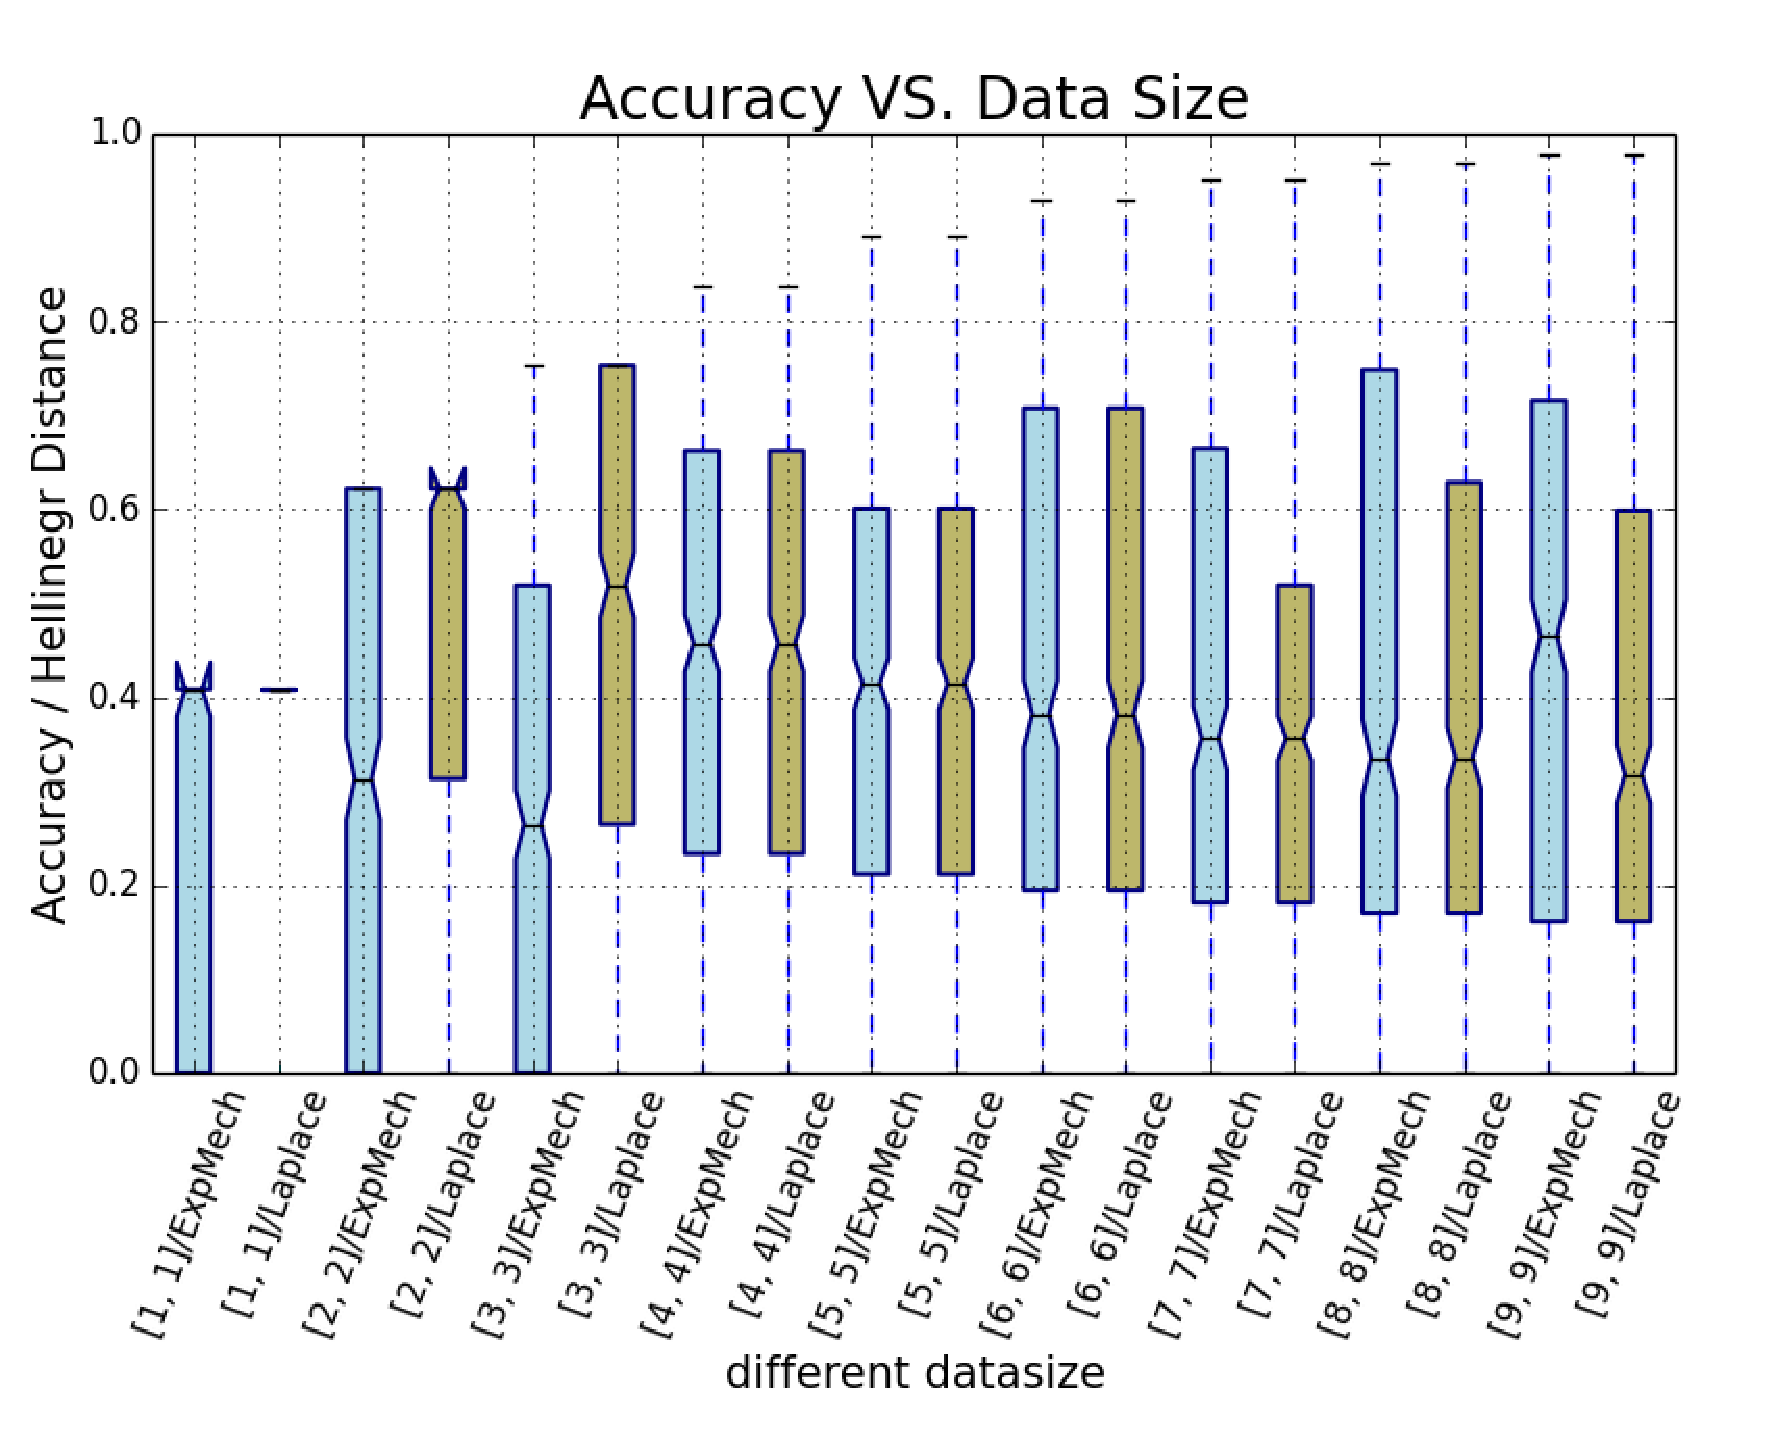
\includegraphics[width=0.3\textwidth]{accuracy_vs_datasize_1_1.eps}}
  \subfigure[three dimensions with $\dirichlet (1,1,1)$ prior distribution]{
    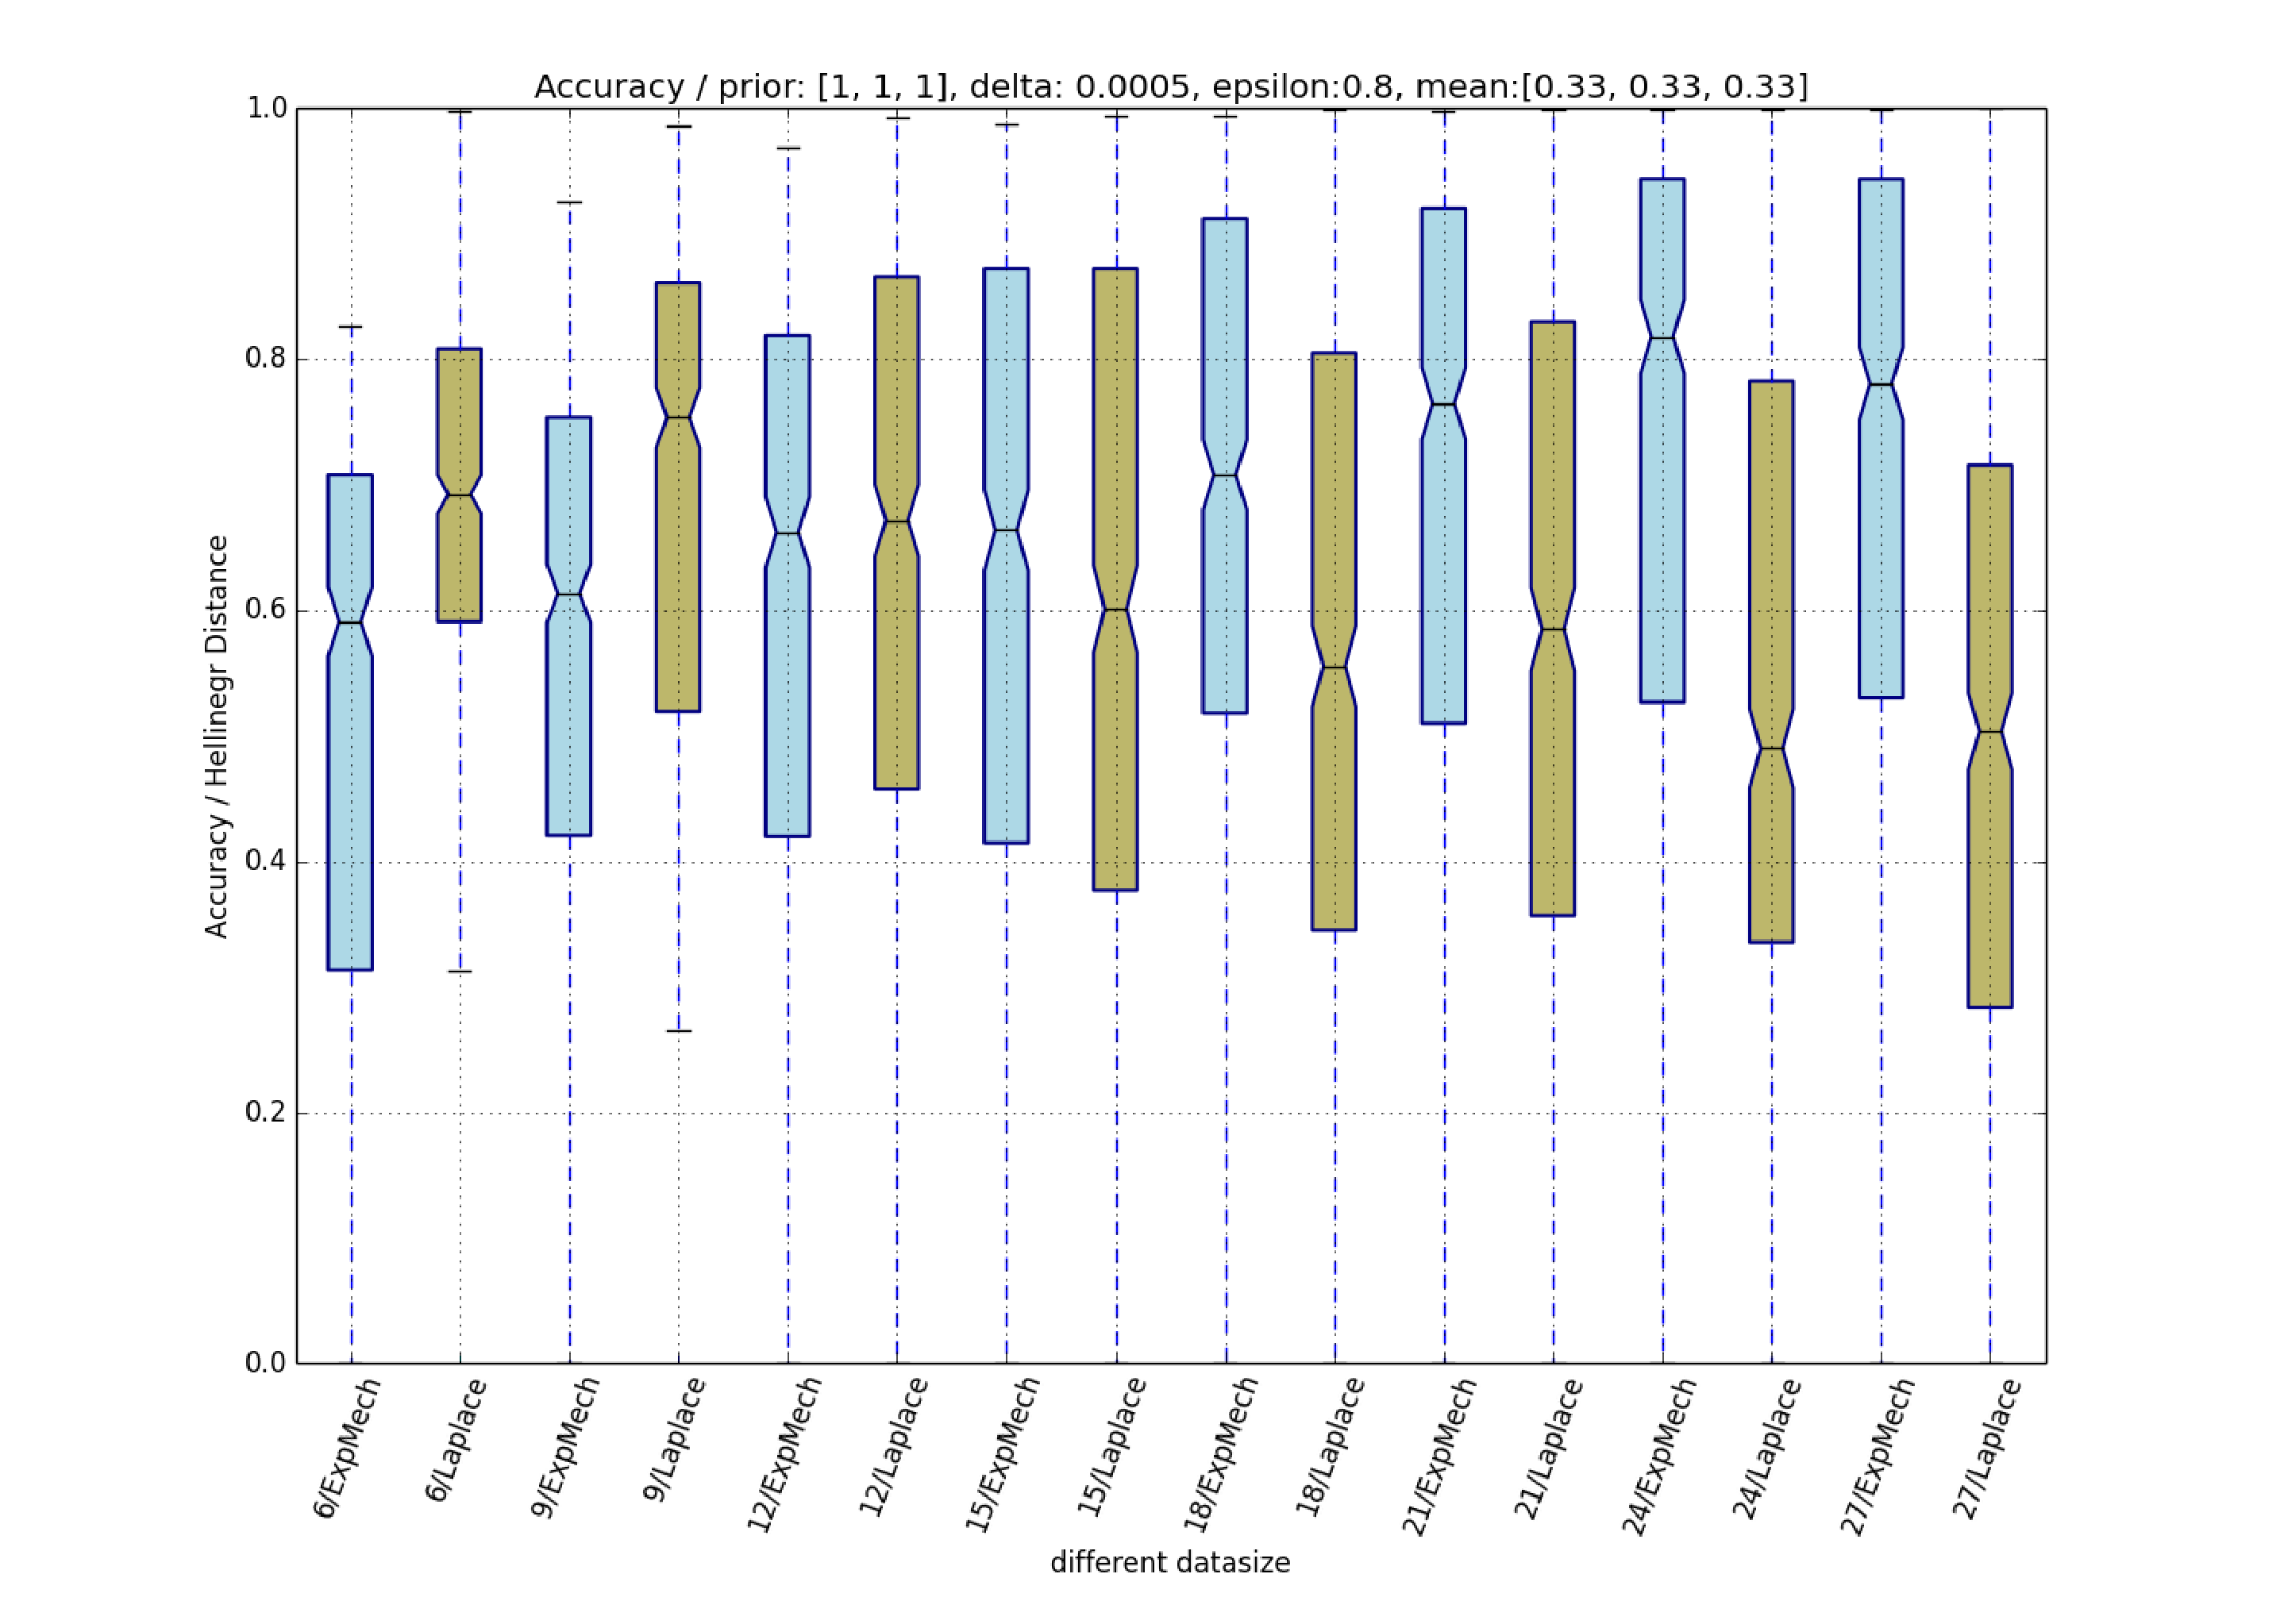
\includegraphics[width=0.3\textwidth]{accuracy_vs_datasize_1_1_1.eps}} 
\caption{Accuracy measurement based on Hellinger distance wrt. different datasizes. Settings: observed data are uniformly distributed, $\epsilon = 0.8$ and $\delta = 0.00000001$}
\label{fig_vs_datasize}
\end{center}
\end{figure}

In Fig. \ref{fig_vs_datasize}, both of the two plots show that when data size go larger, accuracy of our exponential mechanism are decreasing. In Fig. \ref{fig_vs_datasize}(a), when the data size is smaller than 12, we can beta Laplace mechanism but fail when data size larger than or equal to 12. Same as in Fig. \ref{fig_vs_datasize}(b), we can beat Laplace mechanism when data size is smaller than 15 and fail otherwise.

\subsubsection{Accuracy Evaluation wrt. Dimensions}
\label{subsubsec_vs_dimension}


\begin{figure}[ht]
\centering
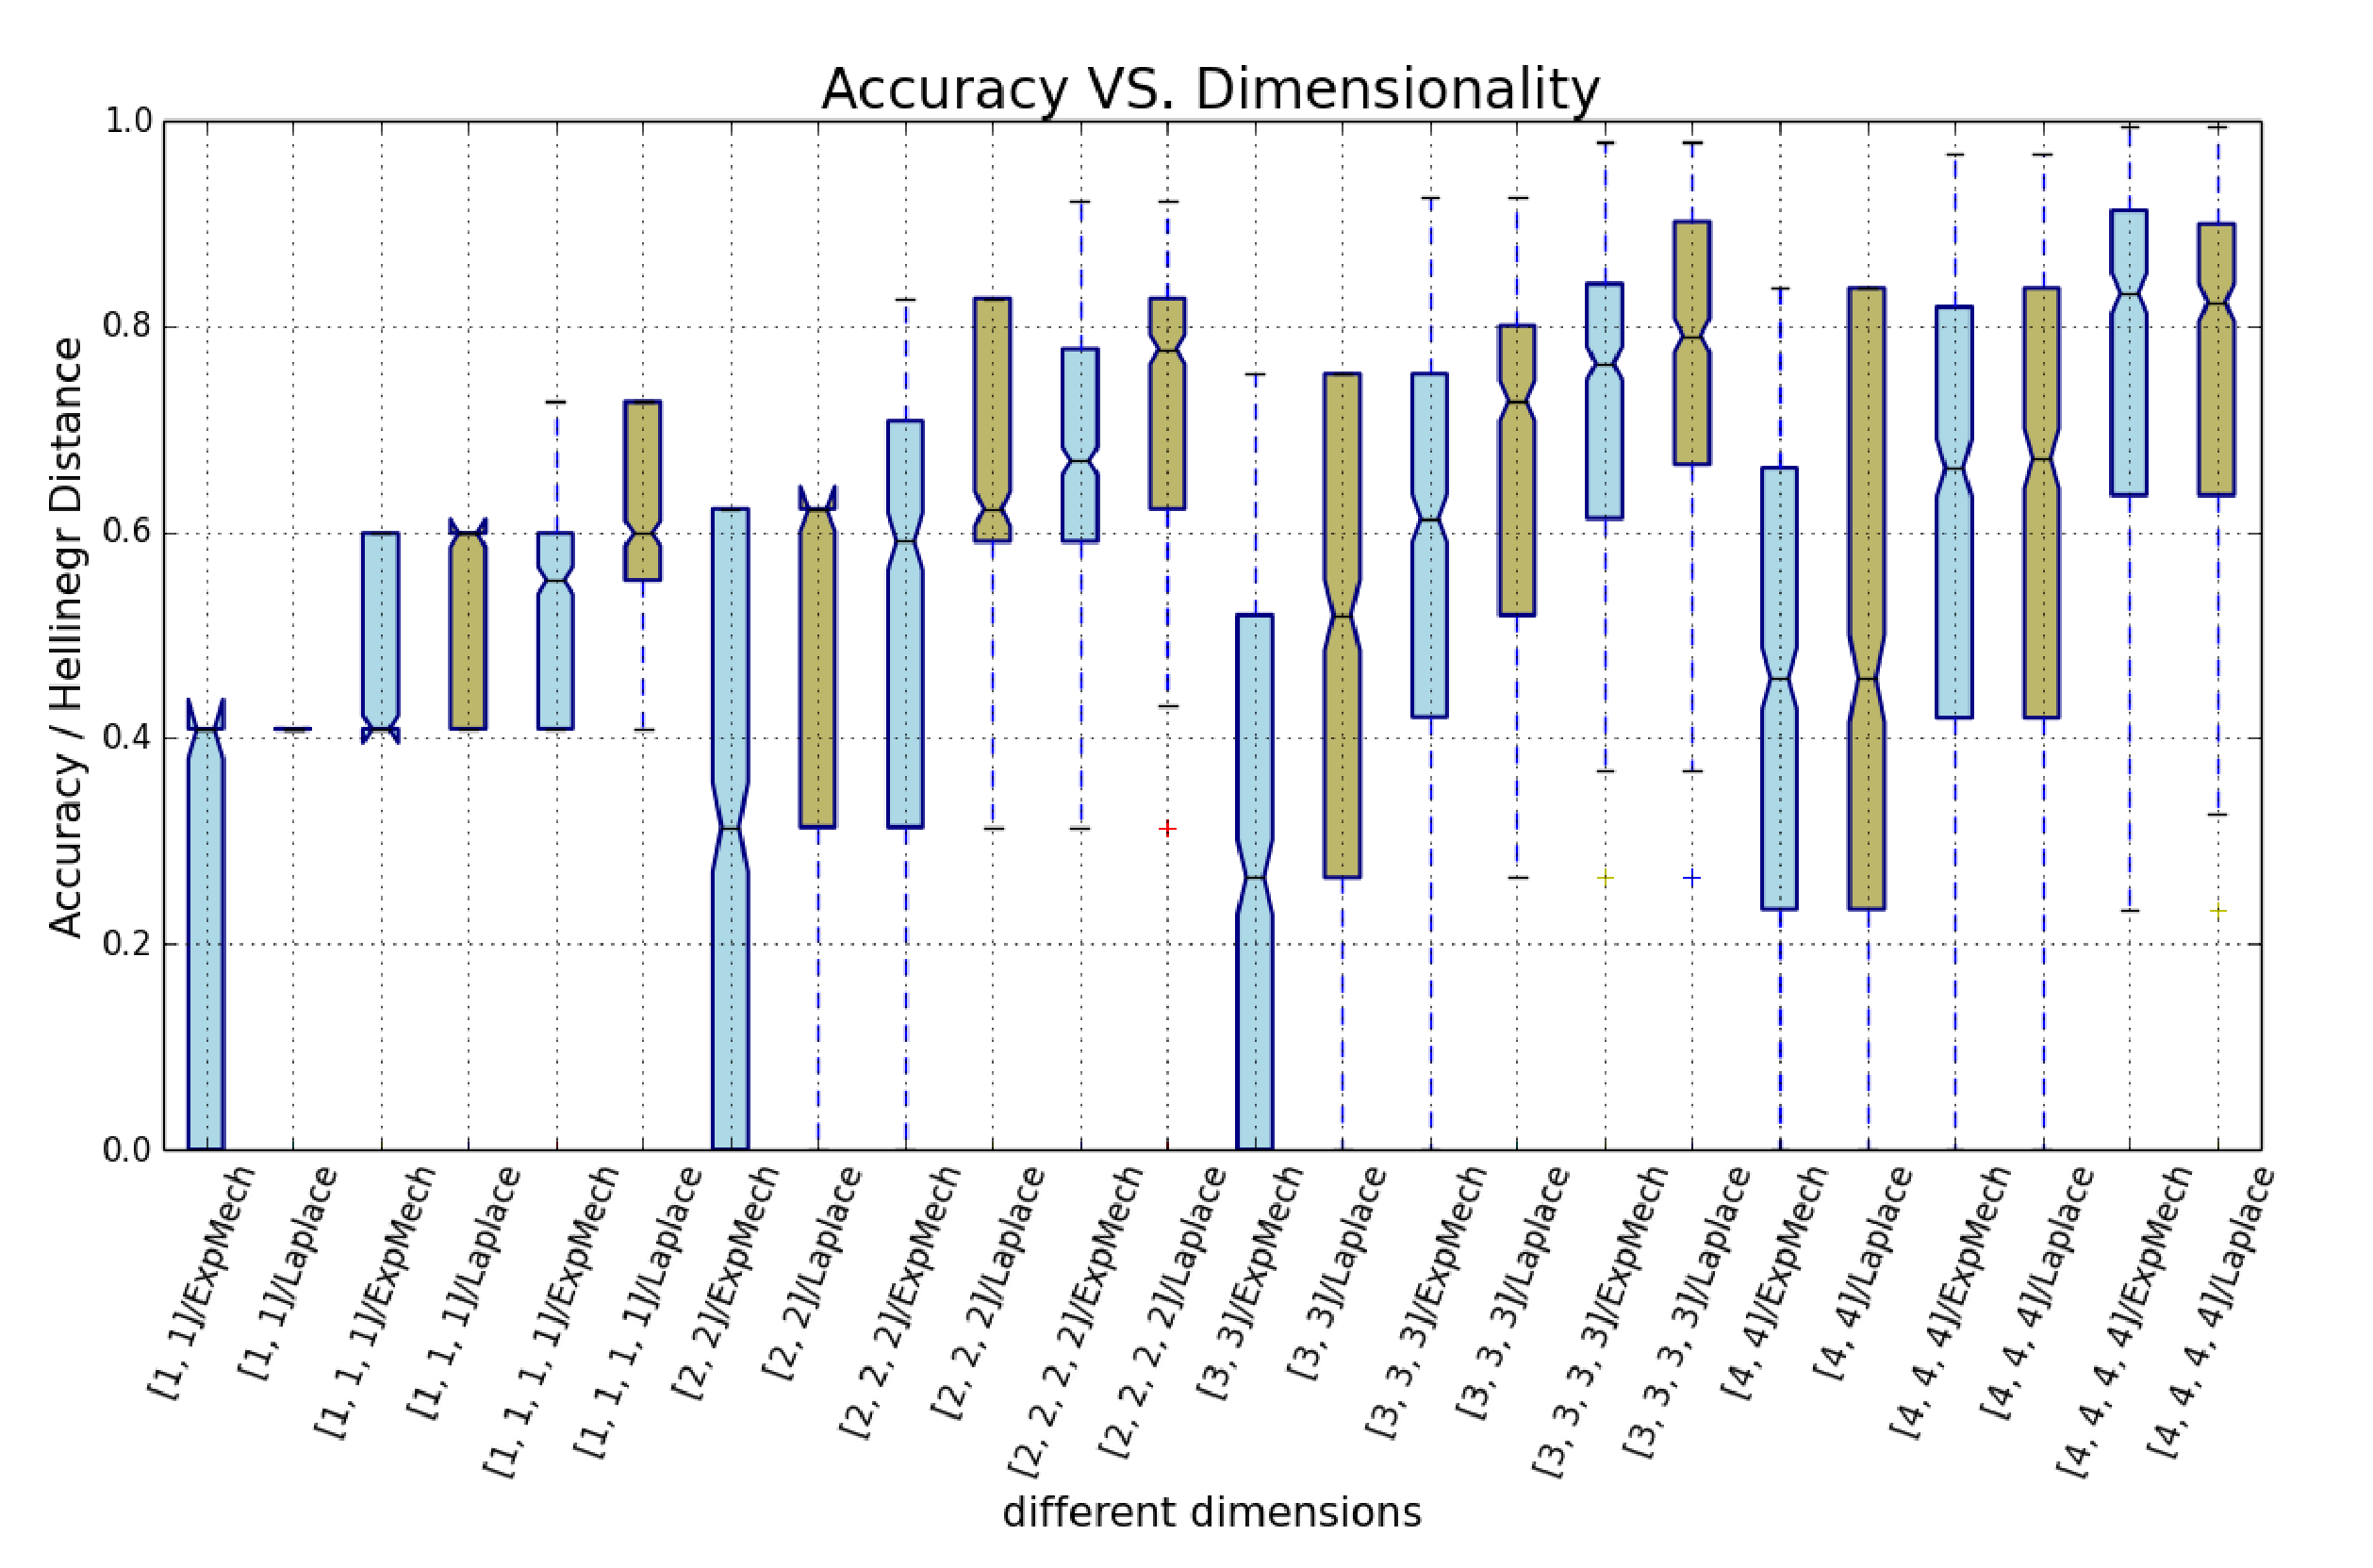
\includegraphics[width=0.45\textwidth]{accuracy_vs_dimension.eps}
\caption{Accuracy measurement based on Hellinger distance wrt. different dimensions and data size. Settings: observed data are uniformly distributed, $\epsilon = 0.8$ and $\delta = 0.00000001$, prior distributions are all $1$ in every dimension}
\label{fig_vs_dimension}
\end{figure}

In Fig. \ref{fig_vs_dimension}, x-axis are observed data sets of different size and dimensions. The plot shows that dimensions have similar influence on our exponential mechanism and the Laplace mechanism. Accuracy of two mechanisms both decrease when dimensions go larger. We will be beat by Laplace mechanism when data size increase but will not be affected when dimensions increase. In other words, dimension has little influence on whether we will beat Laplace mechanism.


\subsubsection{Accuracy Evaluation wrt. Data variance}
\label{subsubsec_vs_variance}

\begin{figure}[ht]
\centering
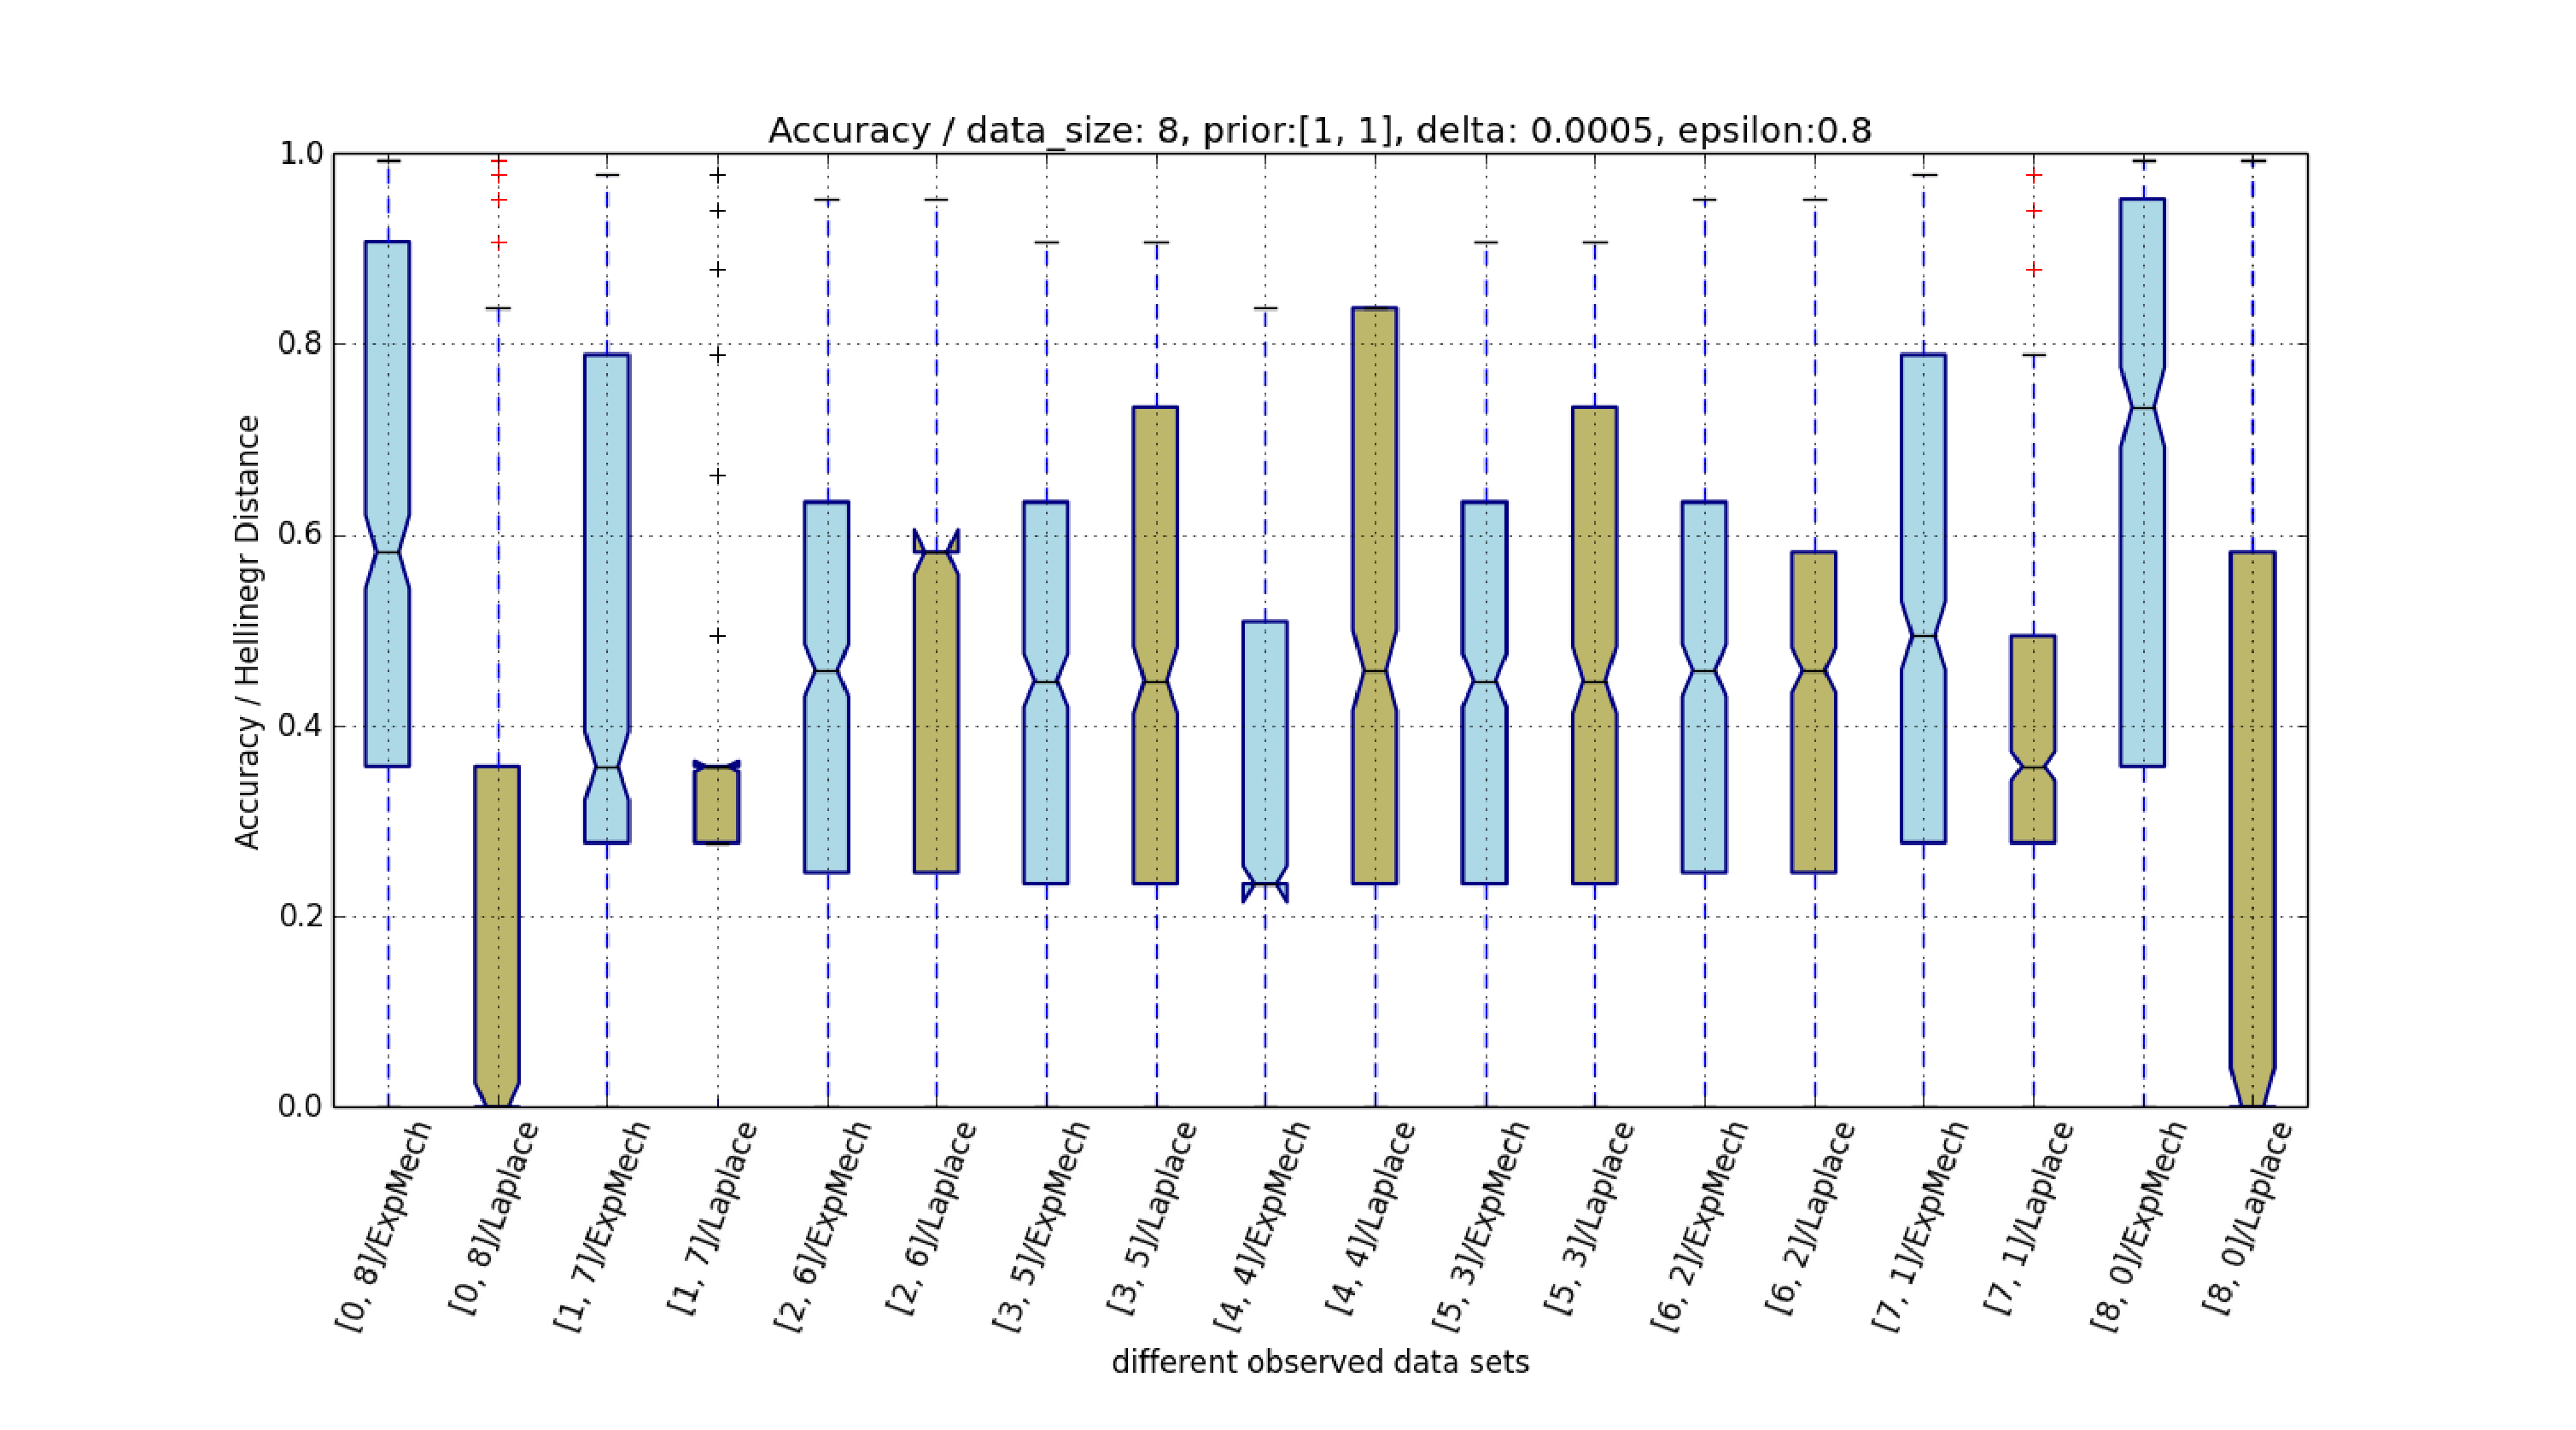
\includegraphics[width=0.45\textwidth]{accuracy_vs_mean_1_1.eps}
\caption{Accuracy measurement based on Hellinger distance wrt. different data variance. Settings: $\epsilon = 0.8$ and $\delta = 0.00000001$, prior distributions are all $1$ in every dimension}
\label{fig_vs_variance}
\end{figure}

In Fig. \ref{fig_vs_variance}, x-axis are observed data sets of different variances (or means). We study this variable under two-dimension $\betad$ distribution in order to be concise. It shows that our mechanism's accuracy is better when data variance go smaller, meanwhile Laplace mechanism go worse. We will beat Laplace mechanism when observed data are more uniformly.



\subsubsection{Accuracy Evaluation wrt. Prior Distribution}
\label{subsubsec_vs_prior}

\begin{figure}[ht]
\centering
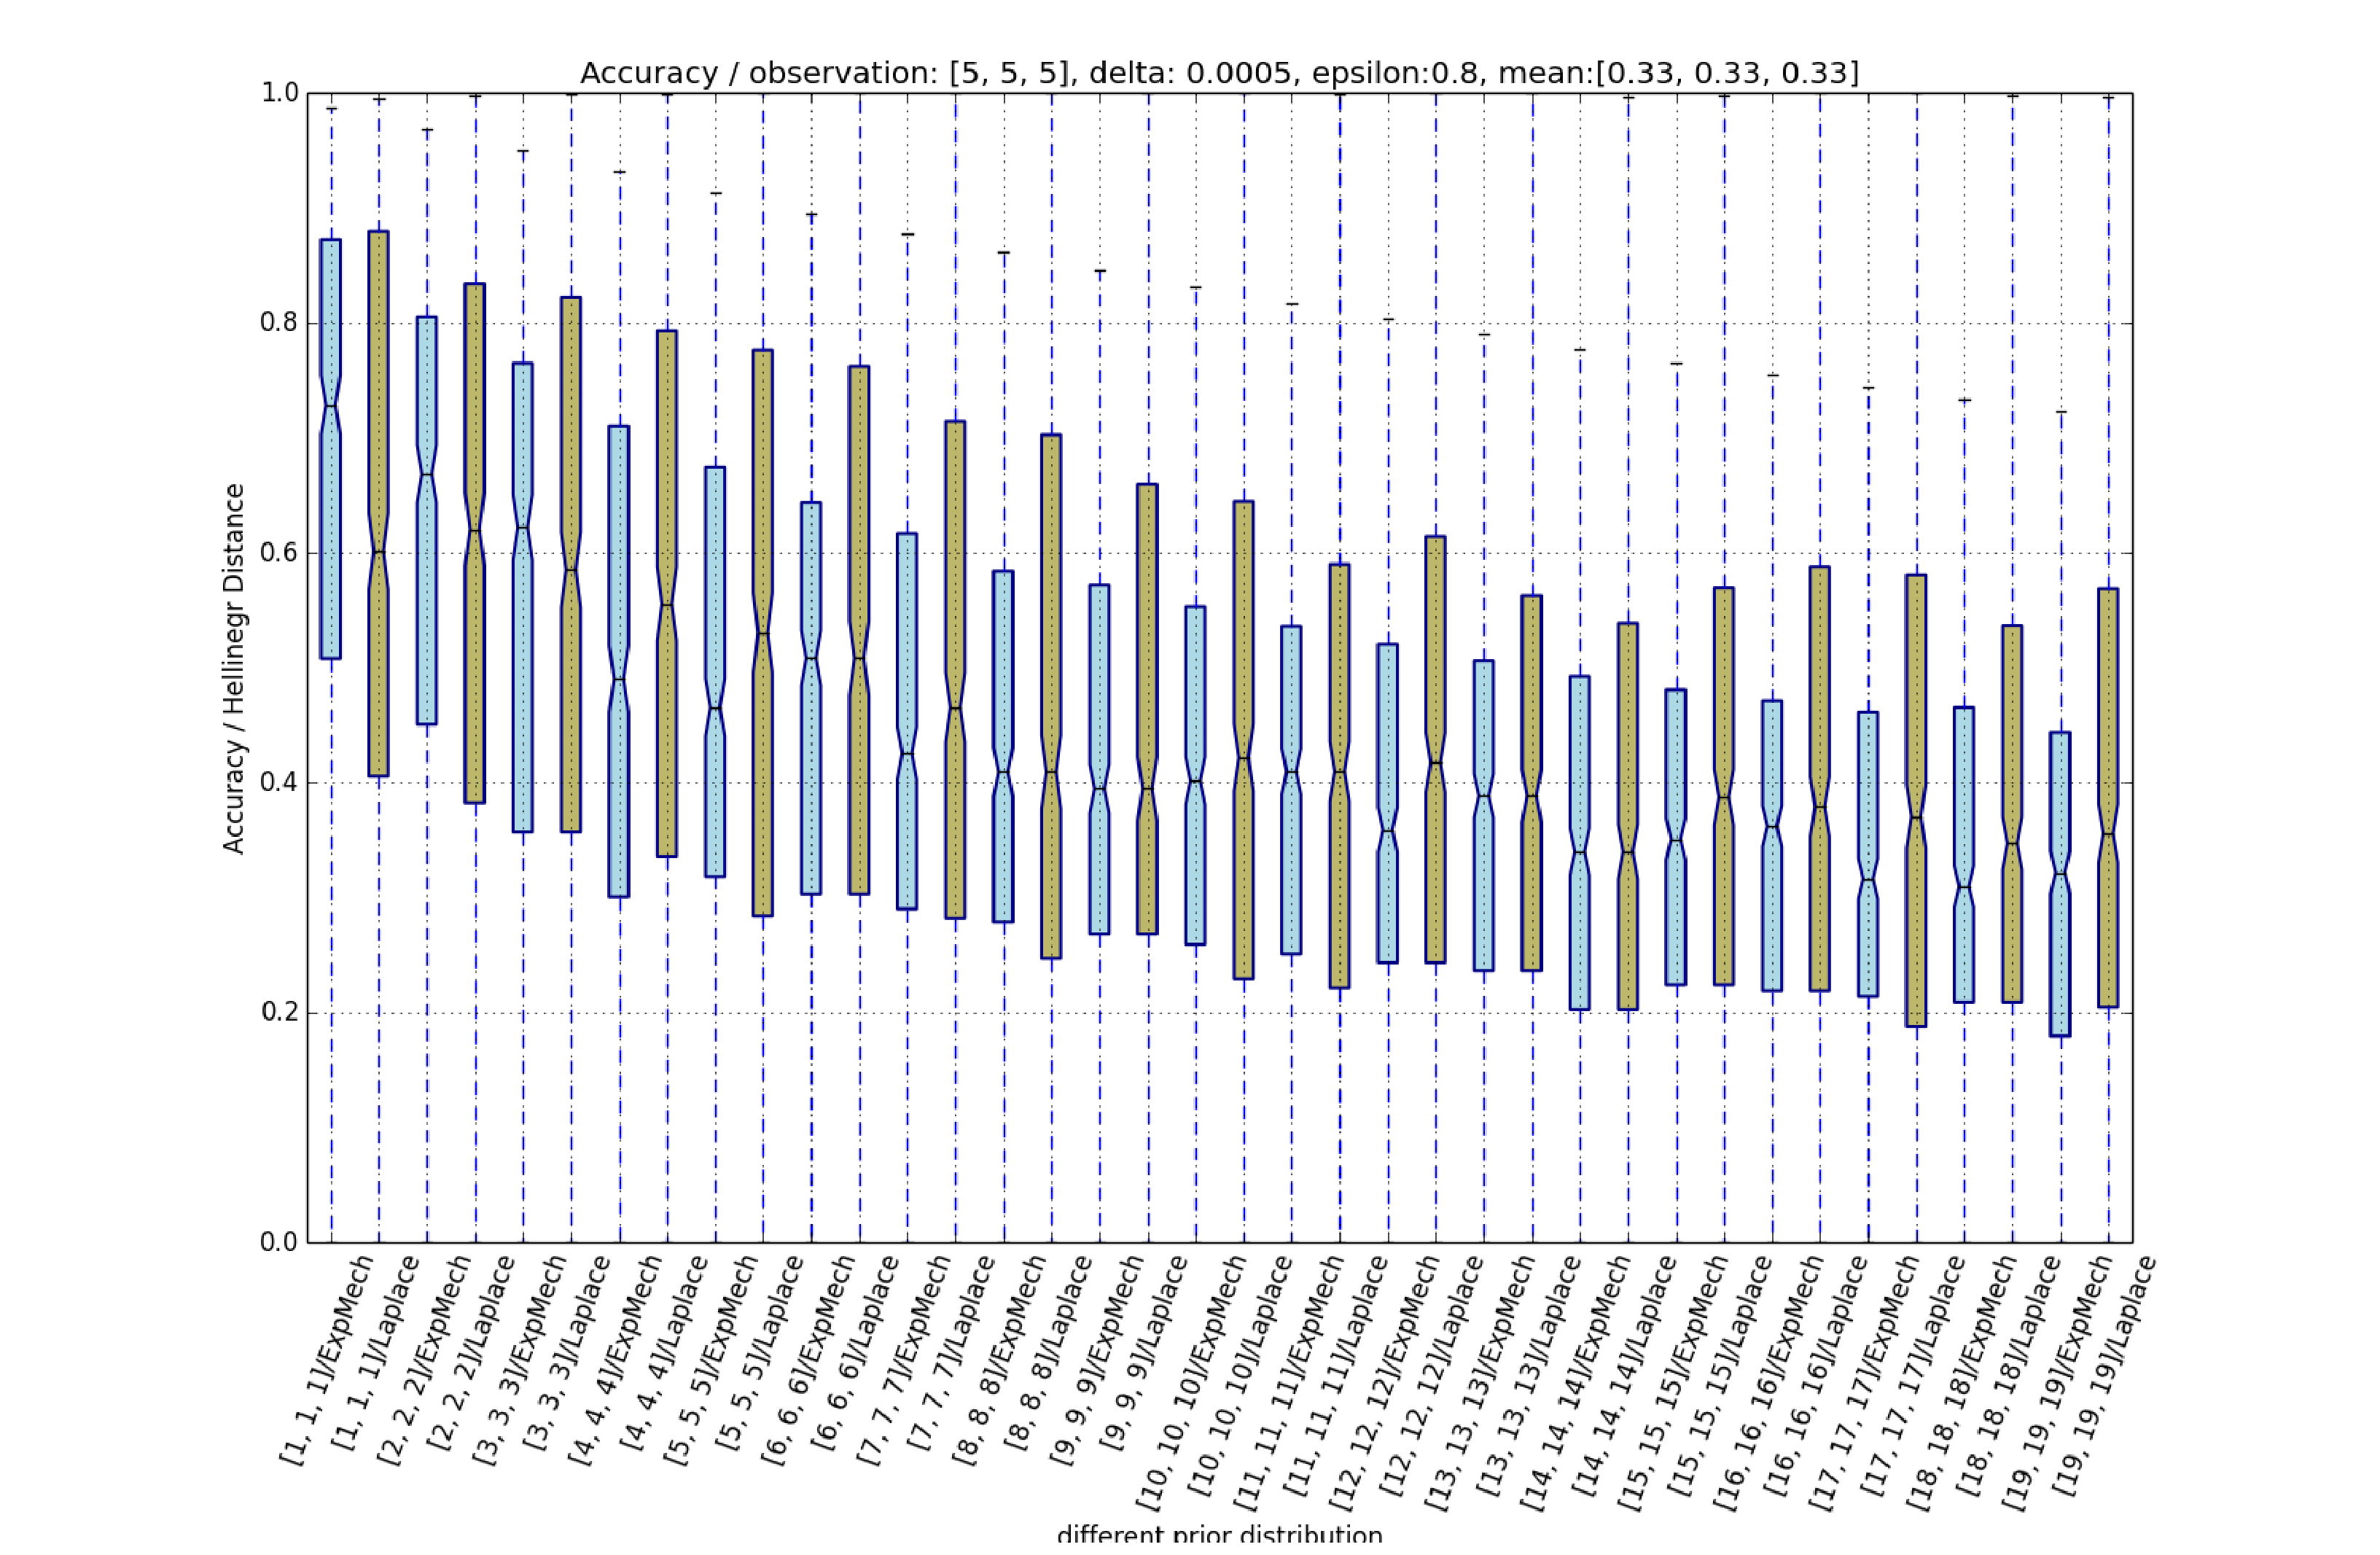
\includegraphics[width=0.45\textwidth]{accuracy_vs_prior_5_5_5.eps}
\caption{Accuracy measurement based on Hellinger distance wrt. different prior distribution. Settings: $\epsilon = 0.8$ and $\delta = 0.00000001$, observed data set is: $[5,5,5]$}
\label{fig_vs_prior}
\end{figure}

In Fig. \ref{fig_vs_prior}, we study this variable under setting that observed data set is $[5,5,5]$ because in Fig. \ref{fig_vs_datasize} Laplace mechanism beat us when data size is 15 and uniformly distributed. The plot shows that in the beginning we cannot beat Laplace but when prior distribution grow larger, we perform better and better and beat Laplace mechanism finally.



% \subsubsection{Accuracy Evaluation wrt. Prior Distribution and Data Variance}
% \label{subsubsec_vs_prior_variance}

% \begin{figure}[ht]
% \centering
% 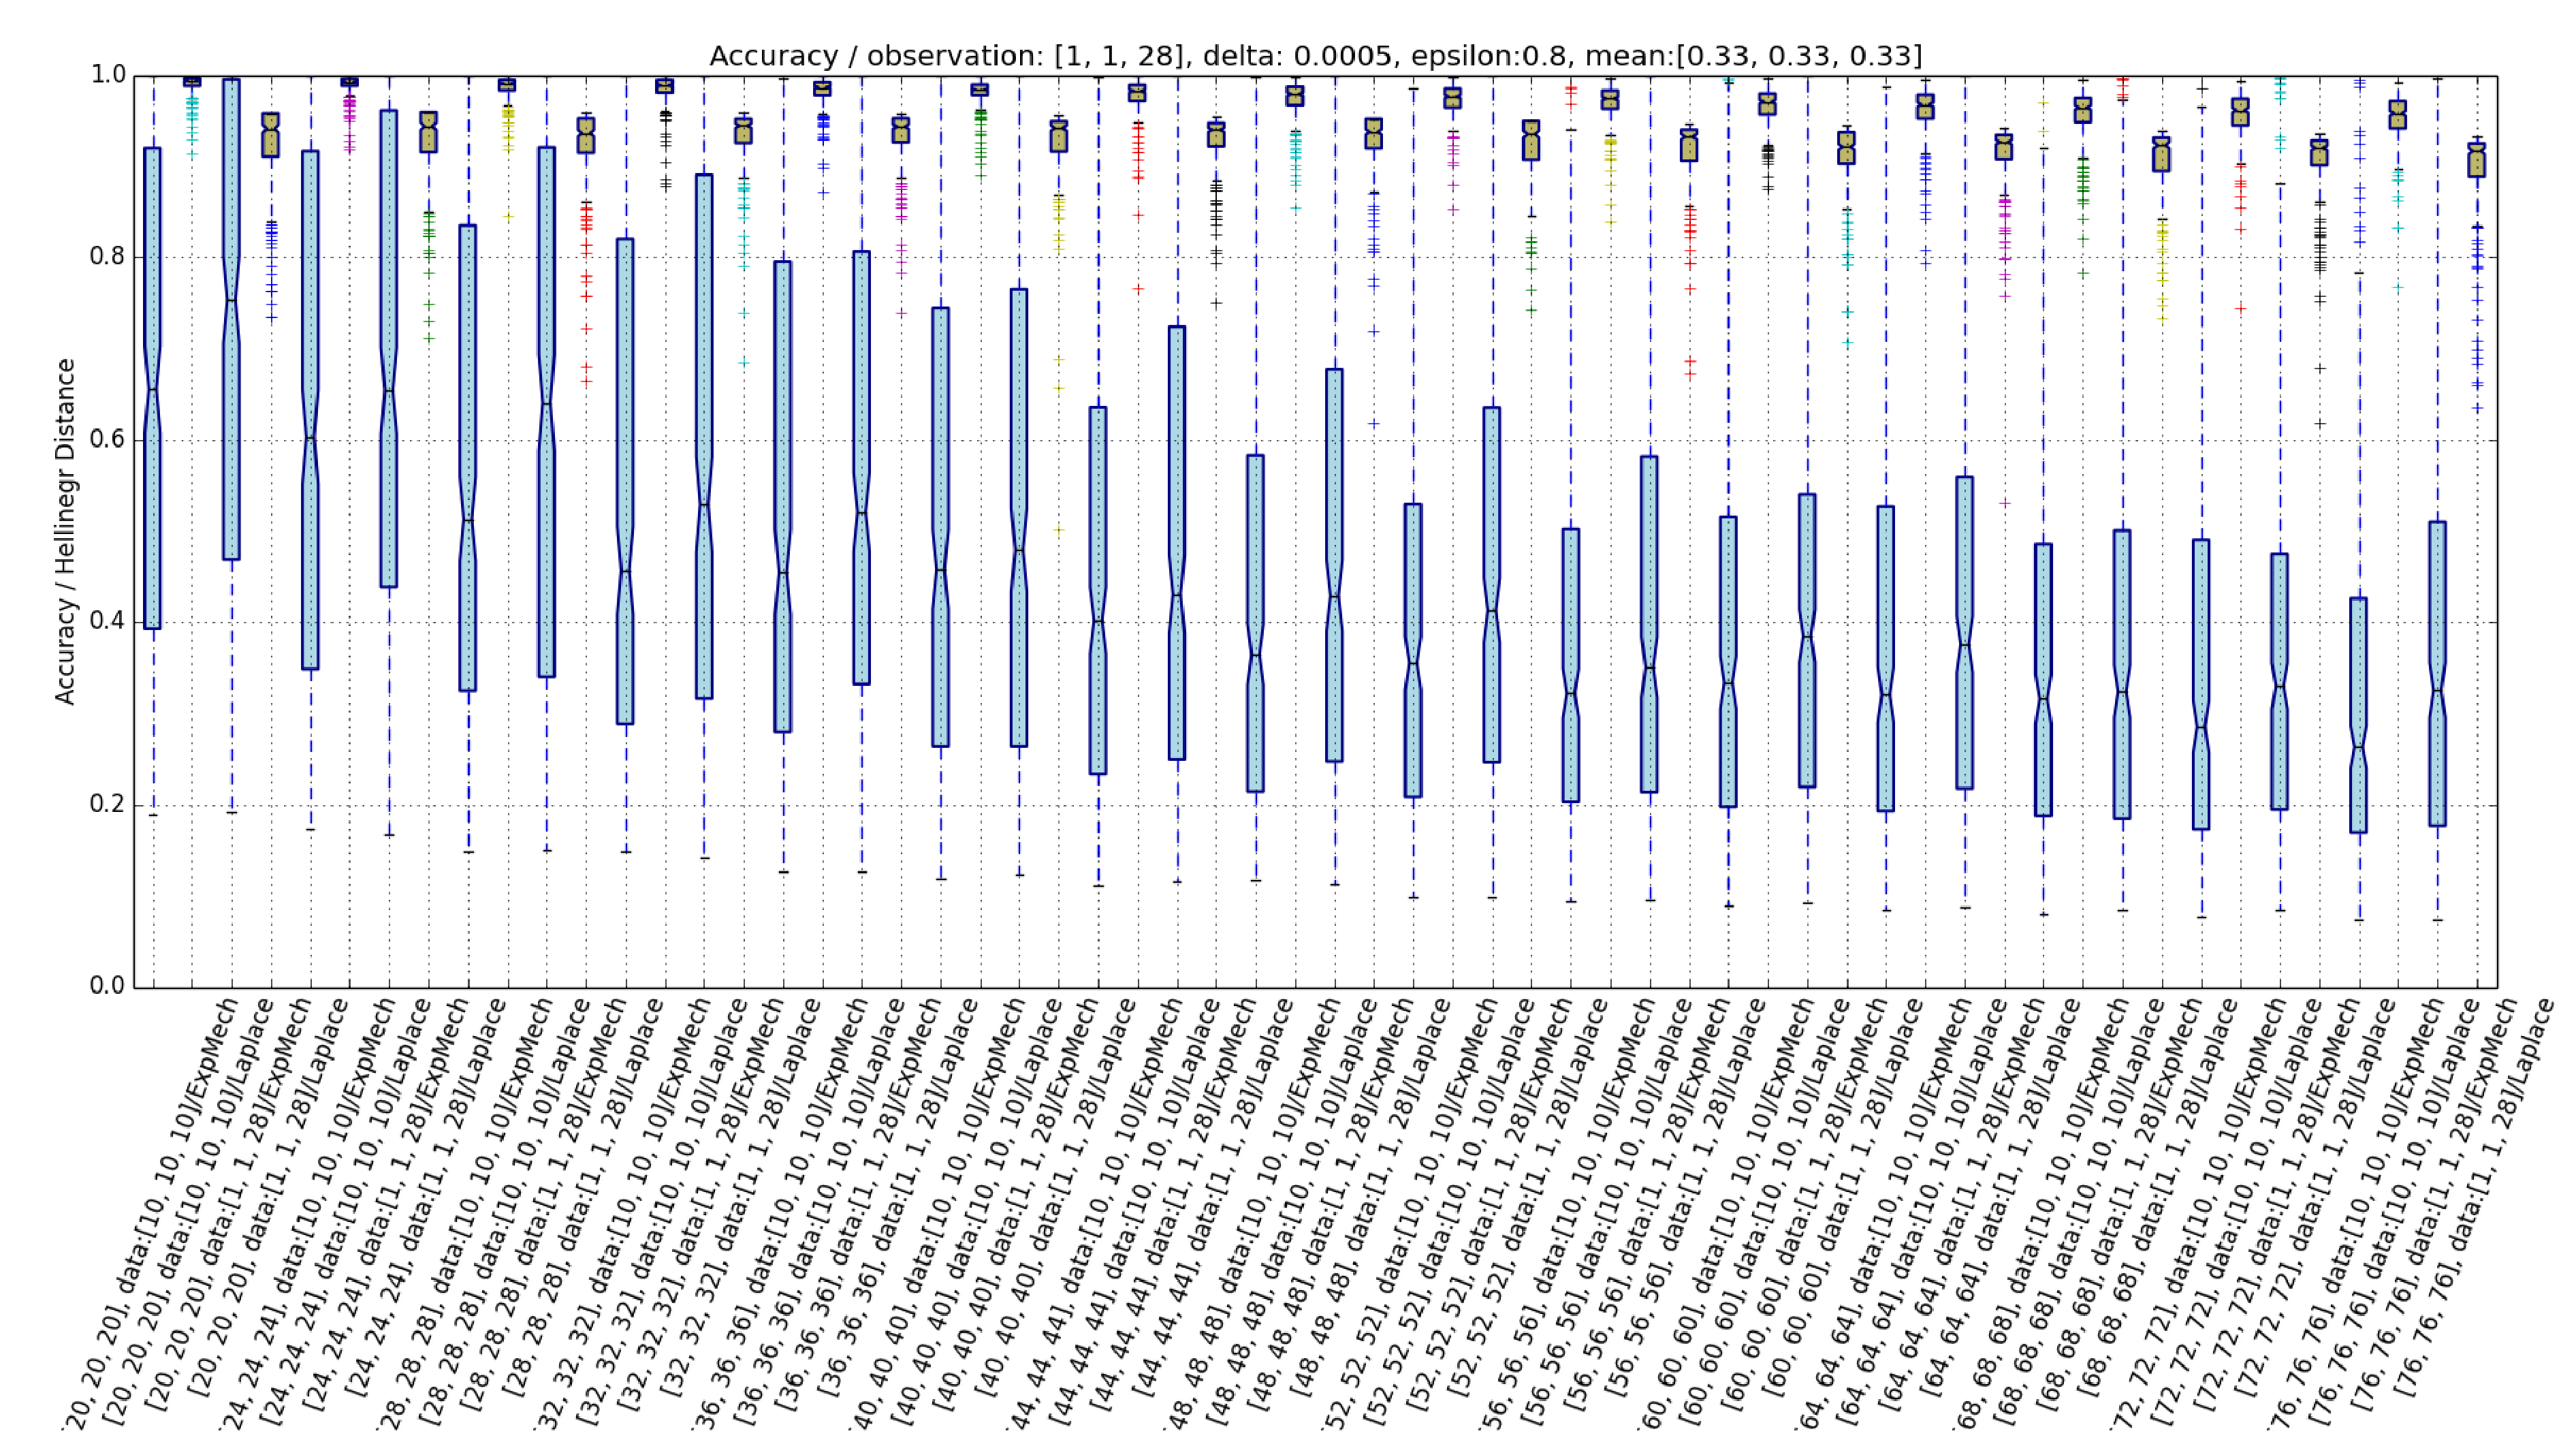
\includegraphics[width=0.45\textwidth]{Accuracy_VS_Prior_mean.eps}
% \caption{Accuracy measurement based on Hellinger distance wrt. different prior distribution and data variances. Settings: $\epsilon = 0.8$ and $\delta = 0.00000001$, observed data sets are $[10,10,10]$ and $[1,1,28]$ and prior distributions are range from $[20,20,20]$ to $[76,76,76]$}
% \label{fig_vs_prior_variance}
% \end{figure}

% Here, we change the prior distribution and data variance in the same time. As shown in Fig. \ref{fig_vs_prior_variance}, our exponential mechanism do better in uniform data set than in edging data set while Laplace mechanism on the contrary. Moreover, our mechanism is improving continuously and significantly as prior distribution increasing while Laplace mechanism isn't.


\section{Conclusions}
We can obtain some preliminary conclusions: 
\begin{enumerate}
	\item We can beat Laplace mechanism when data size is small.
	\item We will beat Laplace mechanism when observed data are more uniformly.
  \item When prior distribution grow larger, we perform better and better and beat Laplace mechanism finally.
\end{enumerate} 

In consequence, we have a better accuracy in small data size, in larger prior and in uniformly data.



\bibliographystyle{ACM-Reference-Format}
\bibliography{bayesian.bib}

\end{document}
 % TODO: replace with your brilliant paper!
% 
%packages
\usepackage{natbib}
\usepackage{amsmath}
\usepackage{amsthm}
\usepackage{mathtools}
\usepackage{mdframed}
\usepackage{subfigure}
\usepackage{booktabs}
% \usepackage{hyperref}
\usepackage{subfigure}
\usepackage{siunitx} % Provides the \SI{}{} and \si{} command for typesetting SI units
\usepackage{graphicx} % Required for the inclusion of images
% \usepackage{natbib} % Required to change bibliography style to APA
\usepackage{datetime}
\usepackage{lscape}
\usepackage{algorithm}
\usepackage{algorithmic}
\usepackage{xspace}
\usepackage[english]{babel} % English language/hyphenation
\usepackage{proof}
\usepackage{booktabs} % Top and bottom rules for tables
\usepackage[colorlinks, allcolors = blue,]{hyperref}
\usepackage{accents}
\usepackage{amsfonts}
\usepackage{stmaryrd}
\usepackage{amsmath,amsthm,amssymb,latexsym} 
\usepackage{microtype}
\usepackage{graphicx}
\usepackage{subfigure}
\usepackage{booktabs} % for professional tables
\usepackage{hyperref}
\usepackage{icml2019}
\usepackage{lipsum}

\usepackage{authblk}


%new commands
\newcommand{\theHalgorithm}{\arabic{algorithm}}
\newtheorem{definition}{Definition}
\usepackage{cancel}
\usepackage[normalem]{ulem}
\newcommand{\dataobs}{\textbf{x}}
\newcommand{\adj}[2]{\textbf{adj}(#1,#2)}
\newcommand{\candidateset}{\mathcal{R}_{\textup{post}}}
\newcommand{\bprior}{\boldsymbol{\beta}_{\textup{prior}}}
\newcommand{\bysinfer}{\mathsf{Infer}}
\newcommand{\betad}{\mathsf{Beta}}
\newcommand{\betaf}{\textup{B}}
\newcommand{\mbetaf}{\boldsymbol{\textup{B}}}
\newcommand{\vtheta}{\boldsymbol{\theta}}
\newcommand{\valpha}{\boldsymbol{\alpha}}
\newcommand{\vbeta}{\boldsymbol{\beta}}
\newcommand{\lapmech}{\mathsf{LSDim}}
\newcommand{\ilapmech}{\mathsf{LSHist}}
\newcommand{\binomial}[2]{\mathsf{Bin}(#1, #2)}
\newcommand{\multinomial}[2]{\mathsf{Mult}(#1, #2)}
\newcommand{\expmech}{\mathsf{EHD}}
\newcommand{\hexpmech}{\mathsf{EHDS}}
\newcommand{\lexpmech}{\mathsf{EHDL}}
\newcommand{\hexpmechd}{\mathsf{expMech}^{D}_{\hellinger}}
\newcommand{\privinfer}{\mathsf{PrivInfer}}
\newcommand{\hlg}{\mathsf{H}}
\newcommand{\dirichlet}[1]{\mathsf{Dir}(#1)}
\newcommand{\alphas}{\boldsymbol{\alpha}}
\newcommand{\xis}{\boldsymbol{\xi}}
\newcommand{\iverson}[1]{[#1]}
\newcommand{\datauni}{\mathcal{X}}
\newcommand{\hellinger}{\mathcal{H}}
\newcommand{\ux}[1]{u(\textbf{x}, {#1})}
\newcommand{\uxadj}[1]{u(\textbf{x}', {#1})}
\newcommand{\cardinality}[2]{\mathcal{C}^{#1}_{#2}}
\newcommand{\range}{\mathcal{O}}
\newcommand{\nomalizer}[1]{\sum\limits_{r'\in \mathcal{R}_{\textup{post}}} \exp \big(\frac{-\epsilon\cdot \mathcal{H} (\mathsf{BI}(#1),r')}{4 \cdot S(#1)}\big)}

\newcommand{\unomalizer}[1]{\sum\limits_{r'\in \mathcal{R}_{\textup{post}}} \exp \big(\frac{-\epsilon\cdot u(#1, r')}{4 \cdot S(#1)}\big)}


\newcommand{\hexpmechPr}[2]{\underset{z \thicksim \hexpmech(#1)}{\Pr}\left[ #2 \right]}
\newcommand{\lapmechPr}[2]{\underset{z \thicksim \lapmech(#1)}{\Pr}\left[ #2 \right]}

\newcommand{\ilapmechPr}[2]{\underset{
{z \thicksim \ilapmech(#1)}
}{\Pr}\left[ #2 \right]}

\newtheorem{thm}{Theorem}[section]

\newtheorem{lem}{Lemma}[section]

\newtheorem{assert}{Assertion}[lem]
\newcommand{\lap}[2]{\mathsf{Lap}(#1, #2)}
\newcommand{\todo}[1]{{\footnotesize \color{red}\textbf{[[ #1 ]]}}}


\section{Problem Statement}
Our research is based on an observation that under different measurement, mechanisms usually have different accuracy behavior. When adding noise according to a certain measurement, mechanism' accuracy behavior will be better than when adding noise according to other measurements. Here we study the private Bayesian inference based on Hellinger distance measurement. Showing that our newly-designed mechanism adding noise according to Hellinger distance performs better than baseline mechanism adding noise according to $l_1$ norm.

\section{Technical Problem Statement}
\label{sec_bayesInfer}

We are studying the Bayesian inference in Beta-Bernoulli systems. So this part we will technically describe our problem under Beta-Bernoulli systems of Bayesian inference. Suppose $\pi(\xis)$ is our prior belief about some parameters or latent variables $\xis$. By using a group of observed data $\textbf{x}$ sizing $n$, the likelihood of this group of data is $Pr(\textbf{x} | \xis)$, we produce a posterior distribution:
\begin{equation*}
Pr(\xis | \textbf{x}) = \frac{Pr(\textbf{x} | \xis) \pi(\xis)}{Pr(\textbf{x})},
\end{equation*}
denoted as $\bysinfer(\textbf{x},\pi(\xis))$ taking an observed data set $\textbf{x} \in \mathcal{X}^n$ (i.e., $\{0,1\}^n$) and a prior distribution $\pi(\xis)$ as input, outputting a posterior distribution of the parameter $\alphas$. For conciseness, when prior is given, we use $\bysinfer(x)$. $n$ is the size of the observed data size.

In Beta-Bernoulli systems, we take a Beta distribution as prior belief for our parameters and latent variables, $\betad(\alpha, \beta)$, where $\pi(\xi) = \betad(\xi | \alpha, \beta) = \frac{\xi^{\alpha} (1 - \xi)^{\beta}}{B(\alphas)}$, and the Bernoulli distribution as the likelihood for $Pr(\textbf{x} | \xi) = \xi^{\sum\limits_{\mathrm{x_i} \in \textbf{x}}\mathrm{x_i}}(1 - \xi)^{n -\sum\limits_{\mathrm{x_i} \in \textbf{x}}\mathrm{x_i}} $. %We are throwing an irregular coin with side $A$ and side $B$. The posterior is computed as $(\alpha + n_1, \beta + n_0)$, where $n_1$ is the appearance time of side $A$ in the observed data set and $n_0$ is the appearance time of the other side.

This can be extended to Dirichlet distribution of $m$ dimensions $\dirichlet(\alphas)$ where $x$ take value from universe $\mathcal{X}$ of size $m$ (i.e., $\mathcal{X} = \{x_1, \cdots, x_m\}$). $\pi(\xis) = \dirichlet(\xis | \alphas) = \frac{\prod_{i = 1}^{m}\xi_i^{\alpha_i}}{B(\alphas)}$, and the likelihood for $Pr(x | \xis)$ is $\prod\limits_{\xi_i \in \xis}\xi_i^{\sum\limits_{\{\mathrm{x}_i|\mathrm{x}_i = x_i\}} \mathrm{x_i}}$.


% We give a inference process based on a concrete example, where we throw an irregular $m$ sides dice. We want to infer the probability of getting each side $\xis$. We get a observed data set $\{s_{k_1}, s_{k_2}, \cdots, s_{k_n}\}$ by throwing the dice $n$ times, where $k_i \in \{1,2,\cdots, m\}$ denotes the side we get when we throw the dice the $i^{th}$ time. The posterior distribution is still a Dirichlet distribution with parameters $(\alpha_1 + n_1, \alpha_2 + n_2, \cdots, \alpha_m + n_m)$, where $n_i$ is the appearance time of the side $i$ in total.

% In the case that $m = 2$, it is reduced to a Beta distribution $\betad(\alpha, \beta)$. The $m$ side dice change into a irregular coin with side $A$ and side $B$. The posterior is computed as $(\alpha + n_1, \beta + n_0)$, where $n_1$ is the appearance time of side $A$ in the observed data set and $n_0$ is the appearance time of the other side.

The posterior belief about parameters $\xis$ is inferred from the group of sensitive data. Because it is usually published in form of a distribution, for example, $\betad(\alpha',\beta'), \cdots,$ itself can relieve a lot of information about sensitive data. So, the sensitive information we want to protect here is the posterior belief, i.e., $Pr(\xis | \textbf{x})$, rather than just a sample drew from it\cite{foulds2016theory}. Then it will be better if we can use a distance over two distributions to measure the accuracy than a distance over just parameters or values when we are protecting a distribution, for instance, Hellinger distance in our paper. When we measure the accuracy between true posterior and protected posterior using Hellinger distance, it would be better we can have a protection mechanism based on Hellinger distance. However, current mechanisms are mainly based on $l_1$ norm by Laplace mechanism \cite{zhang2016differential} \cite{xiao2012bayesian}. That's why we design our exponential mechanism over Hellinger distance to protect the whole posterior distribution.


\section{Baseline Approach - Laplace Mechanism}
\label{sec_lap}
Based on the posterior results from Bayesian inference, we calculate the Laplace mechanism updates on posterior and get the private results under Laplace mechanism. In the case of $m$ dimension Dirichlet distribution, we will add $(m-1)$ i.i.d. Laplace noises $\{| Lap_1 |, | Lap_2 |, \cdots, | Lap_{m-1} |\}$ to the output, where $Lap_i = floor(Y)$, $Y \sim Lap(\frac{2}{\epsilon})$. The private posterior then will be $\dirichlet(\alpha_1 + n_1 + | Lap_1 |, \alpha_2 + n_2 + | Lap_2 |, \cdots, \alpha_m + n - (Lap_1 + \cdots + Lap_{m-1}))$.

\section{Our Approach - Exponential Mechanism with Smooth Sensitivity}
\label{sec_smoo}

% \subsection{Algorithm Setting up}
We define a new mechanism $\hexpmech(x)$ which is similar to the exponential mechanism where we use $\mathcal{R}$ as the set $\betaset$ of beta distributions with integer parameters summing up to $n+2$, as scoring function we use the Hellinger distance from $\bysinfer(x)$, i.e. $\hlg(\bysinfer(x),-)$, and we calibrate the noise to the smooth sensitivity~\cite{nissim2007smooth}. The only difference is in the sensitivity part, since now we use the smooth sensitivity.

\begin{definition}
\label{def_smoo}
The mechanism $\hexpmech(x)$ outputs a candidate $r \in \betaset$ with probability
\begin{equation*}
\underset{z \thicksim \hexpmech(x)}{Pr}[z=r] = \frac
{exp(\frac{-\epsilon\hlg(\bysinfer(x),r)}{2 S_\beta(x)})}
{\Sigma_{r' \in R}\ exp(\frac{-\epsilon \hlg(\bysinfer(x),r')}{2 S_\beta(x)})},
\end{equation*}
where $s_\beta(x)$ is the smooth sensitivity of $\hlg(\bysinfer(x),-)$, calculated by:
\begin{equation*}
S_{\beta}(x) = \max(\Delta_{l}\hlg(\bysinfer(x),-), \max_{y \neq x; y \in D^{n}}(\Delta_{l}\hlg(\bysinfer(y),-)\cdot e^{-\beta d(x,y)})),
\end{equation*}
where $d$ is the Hamming distance between two datasets, and $\beta =
\beta(\epsilon, \delta)$ is a function of $\epsilon$ and $\delta$. 
\end{definition}


In what follows, we will use a correspondence between the probability
 $\underset{z \thicksim \hexpmech(x)}{Pr}[z = r]$ of every
 $r\in\betaset$ and the probability 
 $\underset{z \thicksim \hexpmech(x)}{Pr}[\hlg(\bysinfer(x),z) =
 \hlg(\bysinfer(x),r)]$ for the utility score for $r$. In particular, for every
 $r\in\betaset$ we have:
$$
\underset{z \thicksim \hexpmech(x)}{Pr}[z = r]=
\frac{1}{2}\Big (\underset{z \thicksim \hexpmech(x)}{Pr}[\hlg(\bysinfer(x),z) =
 \hlg(\bysinfer(x),r)]\Big )
$$
To see this, it is enough to notice that: $\underset{z \thicksim \hexpmech(x)}{Pr}[z = r]$ is proportional too $\hlg(\bysinfer(x),r)$, i.e., $u(x,z)$. We can derive, if $u(r,x) = u(r',x)$ then $\underset{z \thicksim \hexpmech(x)}{Pr}[z = r] = \underset{z \thicksim \hexpmech(x)}{Pr}[z = r']$. We assume the number of candidates $z \in \mathcal{R}$ that satisfy $u(z,x) = u(r,x)$ is $|r|$, we have  $\underset{z \thicksim \hexpmech(x)}{Pr}[u(z,x) = u(r,x)] = |r| \underset{z \thicksim \hexpmech(x)}{Pr}[z = r]$. Because Hellinger distance  $\hlg(\bysinfer(x),z)$ is axial symmetry, where the $\bysinfer(x)$ is the symmetry axis. It can be infer that $|z| = 2$ for any candidates, apart from the true output, i.e., $\underset{z \thicksim \hexpmech(x)}{Pr}[u(z,x) = u(r,x)] = 2 \underset{z \thicksim \hexpmech(x)}{Pr}[z = r]$. This parameter can be eliminate in both sides in proof.

In our private Bayesian inference mechanism, we set the $\beta$ as $\ln(1 - \frac{\epsilon}{2 \ln (\frac{\delta}{2 (n + 1)})})$. 





% \subsection{Sliding Property of Exponential Mechanism}
% \begin{lem}
% Consider the exponential mechanism  $\sexpmech(x,u,\mathcal{R})$
% calibrated on the smooth sensitivity. Let $\lambda = f(\epsilon,
% \delta)$, $\epsilon\geq 0$ and $|\delta| < 1$. Then, the following \emph{sliding property} holds:
% \begin{equation*}
% \underset{r \thicksim \hexpmech(x)}{Pr}[u(r,x) = \hat{s}]
% \leq
% e^{\frac{\epsilon}{2}} \underset{r \thicksim \hexpmech(x)}{Pr}[u(r,x) = (\Delta + \hat{s})] + \frac{\delta}{2},
% \end{equation*}

% \end{lem}

% \begin{proof}

% We denote the normalizer of the probability mass in $\hexpmech(x)$: $\sum_{r' \in \mathcal{R}}exp(\frac{\epsilon u(r',x)}{2 S(x)})$ as $NL(x)$:
% \begin{equation*}
% \begin{split}
% LHS 
%   = \underset{r \thicksim \hexpmech(x)}{Pr}[u(r,x) = \hat{s}]
% & = \frac{exp(\frac{\epsilon \hat{s}}{2 S(x)})}{NL(x)}\\
% & = \frac{exp(\frac{\epsilon (\hat{s} + \Delta - \Delta)}{2 S(x)})}{NL(x)}\\
% & = \frac{exp(\frac{\epsilon (\hat{s} + \Delta)}{2 S(x)} + \frac{- \epsilon \Delta}{2 S(x)})}{NL(x)}\\
% & = \frac{exp(\frac{\epsilon (\hat{s} + \Delta)}{2 S(x)})}{NL(x)} \cdot e^{\frac{- \epsilon \Delta}{2 S(x)})}.\\
% \end{split}
% \end{equation*}

% By bounding the $\Delta \geq -S(x)$, we can get:

% \begin{equation*}
% \begin{split}
% \frac{exp(\frac{\epsilon (\hat{s} + \Delta)}{2 S(x)})}{NL(x)} \cdot e^{\frac{- \epsilon \Delta}{2 S(x)}}
% & \leq \frac{exp(\frac{\epsilon (\hat{s} + \Delta)}{2 S(x)})}{NL(x)} \cdot e^{\frac{\epsilon}{2}}\\
% &  =  e^{\frac{\epsilon}{2}} \underset{z \thicksim \hexpmech(x)}{Pr}[u(r,x) = (\Delta + \hat{s})] \leq RHS\\
% \end{split}
% \end{equation*}

% \end{proof}

% \subsection{Dilation Property of Exponential Mechanism}
% \begin{lem}
% for any exponential mechanism $\hexpmech(x)$, $\lambda < |\beta|$, $\epsilon$, $|\delta| < 1$ and $\beta \leq \ln(1 - \frac{\epsilon}{2 \ln (\frac{\delta}{2 (n + 1)})})$, the dilation property holds:

% \begin{equation*}
% \underset{z \thicksim \hexpmech(x)}{Pr}[u(z,x) = c]
% \leq
% e^{\frac{\epsilon}{2}} \underset{z \thicksim \hexpmech(x)}{Pr}[u(z,x) = e^{\lambda} c] + \frac{\delta}{2},
% \end{equation*}
% where the sensitivity in mechanism is still smooth sensitivity as above.
% \end{lem}

% \begin{proof}

% The sensitivity is always greater than 0, and our utility function $-\hlg(\bysinfer(x),z)$ is smaller than zero, i.e., $u(z,x) \leq 0$, we need to consider two cases where $\lambda < 0$, and $\lambda > 0$:

% We set the $h(c) = Pr[u(\hexpmech(x)) = c] = 2\frac{exp(\frac{\epsilon z}{2 S(x)})}{NL(x)}$.

% We first consider $\lambda < 0$. In this case, $1 < e ^ {\lambda}$, so the ratio $\frac{h(c)}{h(e^{\lambda}c)} = \frac{exp(\frac{\epsilon c}{2 S(x)})}{exp(\frac{\epsilon (c \cdot e^{\lambda})}{2 S(x)})}$ is at most $\frac{\epsilon}{2}$.

% Next, we proof the dilation property for $\lambda > 0$, The ratio of $\frac{h(c)}{h(e^{\lambda}c)}$ is $\exp(\frac{\epsilon}{2} \cdot \frac{u(\hexpmech(x)) (1 - e^{\lambda})}{S(x)})$. Consider the event $G = \{ \hexpmech(x) : u(\hexpmech(x)) \leq \frac{S(x)}{(1 - e^{\lambda})}\}$. Under this event, the log-ratio above is at most $\frac{\epsilon}{2}$. The probability of $G$ under density $h(c)$ is $1 - \frac{\delta}{2}$. Thus, the probability of a given event $z$ is at most $Pr[c \cap G] + Pr[\overline{G}] \leq e^{\frac{\epsilon}{2}} Pr[e^{\lambda}c \cap G] + \frac{\delta}{2} \leq e^{\frac{\epsilon}{2}} Pr[e^{\lambda}c] + \frac{\delta}{2}$.\\


% \textbf{Detail proof:}
% \begin{itemize}

% 	\item $\lambda < 0$

% 		The left hand side will always be smaller than 0 and the right hand side greater than 0. This will always holds, i.e.
% 		\begin{equation*}
% 		\end{equation*}
% 	\item $\lambda > 0$


% Because $\hat{s} = u(r)$ where $r \thicksim \hexpmech(x)$, we can substitute $\hat{s}$ with $u(\hexpmech(x))$. Then, what we need to proof under the case $\lambda > 0$ is:
% \begin{equation*}
% u(\hexpmech(x)) \leq \frac{S(x)}{(1 - e ^ {\lambda})}
% \end{equation*}
% By applying the accuracy property of exponential mechanism, we bound the probability that the equation holds with probability:
% \begin{equation*}
% \begin{split}
% Pr[u(\hexpmech(x)) \leq \frac{S(x)}{(1 - e ^ {\lambda})}] 
% & \leq \frac{|\mathcal{R}|exp(\frac{\epsilon S(x)}{(1 - e ^ {\lambda})}/2 S(x))}{|\mathcal{R}_{OPT}| exp(\epsilon OPT_{u(x)}/2 S(x))}\\
% \end{split}
% \end{equation*}

% In our Bayesian Inference mechanism, the size of the candidate set $\mathcal{R}$ is equal to the size of observed data set plus 1, i.e., $n + 1$, and $OPT_{u(x)} = 0$, then we have:
% \begin{equation*}
% \begin{split}
% Pr[u(\hexpmech(x)) \leq \frac{S(x)}{(1 - e ^ {\lambda})}] 
% & = (n + 1)exp(\frac{\epsilon S(x)}{(1 - e ^ {\lambda})}/2 S(x))\\
% & = (n + 1)exp(\frac{\epsilon}{2 (1 - e ^ {\lambda})})\\
% \end{split}
% \end{equation*}

% When we set $\lambda \leq \ln(1 - \frac{\epsilon}{2 \ln (\frac{\delta}{2 (n + 1)})})$, it is easily to derive that $Pr[u(\hexpmech(x)) \leq \frac{S(x)}{(1 - e ^ {\lambda})}] \leq \frac{\delta}{2}$.

% \end{itemize}

% \end{proof}

% \subsection{Privacy Analysis}
% \begin{lem}
% \label{lem_hexpmech_privacy}
% $\hexpmech$ is $(\epsilon, \delta)$-differential privacy.
% \end{lem}

% \begin{proof}
% of Lemma \ref{lem_hexpmech_privacy}: For all neighboring $x, y \in D^n$ and all sets $\mathcal{S}$, we need to show that:
% \begin{equation*}
% \underset{z \thicksim \hexpmech(x)}{Pr}[ z \in \mathcal{S}] \leq e^{\epsilon} \underset{z \thicksim \hexpmech(y)}{Pr}[z \in \mathcal{S}] + \delta. 
% \end{equation*}
% Given that $2\Big( \underset{z \thicksim \hexpmech(x)}{Pr}[ z \in \mathcal{S}]\Big) = \underset{z \thicksim \hexpmech(x)}{Pr}[ u(x,z) \in \mathcal{U}]$, let $\mathcal{U}_1 = \frac{u(y,z) - u(x,z)}{S(x)}$, $\mathcal{U}_2 = \mathcal{U} + \mathcal{U}_1$ and $\mathcal{U}_3 = \mathcal{U}_2 \cdot \frac{S(x)}{S(y)} \cdot \ln(\frac{NL(x)}{NL(y)})$. Then,

% \begin{equation*}
% \begin{split}
% 2\Big( \underset{z \thicksim \hexpmech(x)}{Pr}[ z \in \mathcal{S}]\Big)
% & = \underset{z \thicksim \hexpmech(x)}{Pr}[ u(x,z) \in \mathcal{U}]\\
% & \leq e^{\epsilon / 2} \cdot \underset{z \thicksim \hexpmech(x)}{Pr}[ u(x,z) \in \mathcal{U}_2]\\
% & \leq e^{\epsilon} \cdot \underset{z \thicksim \hexpmech(x)}{Pr}[ u(x,z) \in \mathcal{U}_3] + e^{\epsilon/2} \cdot \frac{\delta'}{2}\\
% & = e^{\epsilon} \cdot \underset{z \thicksim \hexpmech(y)}{Pr}[ u(y,z) \in \mathcal{U}] + \delta = 2\Big( e^{\epsilon} \cdot \underset{z \thicksim \hexpmech(x)}{Pr}[ z \in \mathcal{S}] \Big) + \delta\\
% \end{split}
% \end{equation*}

% The first inequality holds by the sliding property, since the $\mathcal{U}_1 \geq -S(x)$. The second inequality holds by the dilation property, since $\frac{S(x)}{S(y)} \cdot \ln(\frac{NL(x)}{NL(y)}) \leq 1 - \frac{\epsilon}{2 \ln (\frac{\delta}{2 (n + 1)})}$.

% \end{proof}

\section{Preliminary Experimental Results}
\label{sec_experiment}


\subsection{Accuracy Trade-off Evaluation wrt. Different Variables}
\label{subsec_vs_variables}

In this section, we evaluate the accuracy wrt. four variables, including data size, dimension, data variance and prior distribution, and some combinations of these variables. We experiment 1000 times under each value of variables and produce 4-quantile plots for each variable. In following 4-quantile plots, the y-axis is accuracy measured by Hellinger distance, x-axis is different value of variables. The blue boxes in plots represent our exponential mechanism and the next yellow box represents the Laplace mechanism under the same setting.

\subsubsection{Accuracy Evaluation wrt. Datasize}
\label{subsubsec_vs_datasize}

\begin{figure}[ht]
\begin{center}
\centering
  \subfigure[two dimensions with $\betad (1,1)$ prior distribution]{
    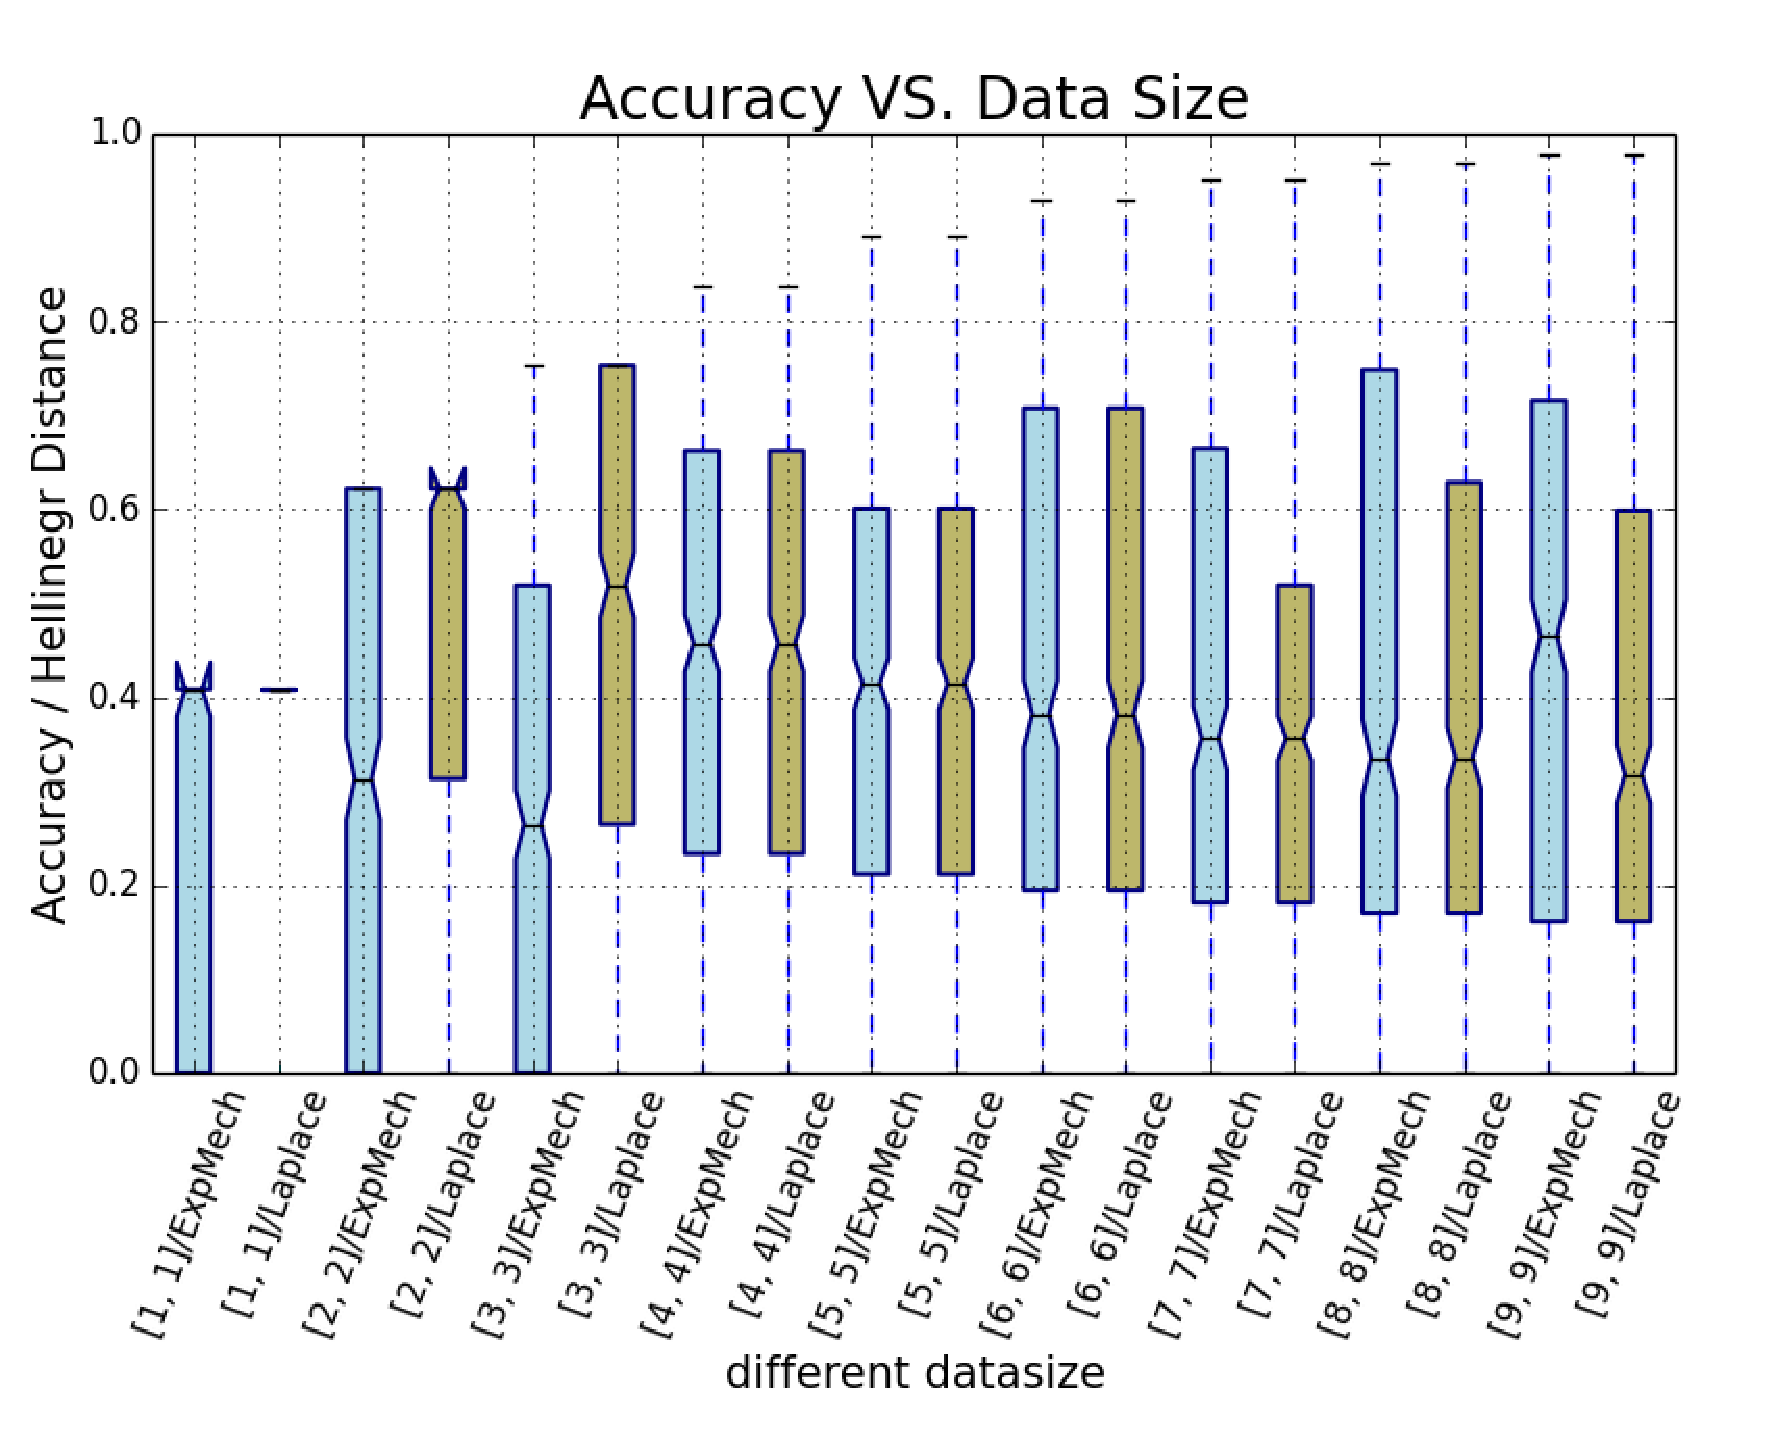
\includegraphics[width=0.3\textwidth]{accuracy_vs_datasize_1_1.eps}}
  \subfigure[three dimensions with $\dirichlet (1,1,1)$ prior distribution]{
    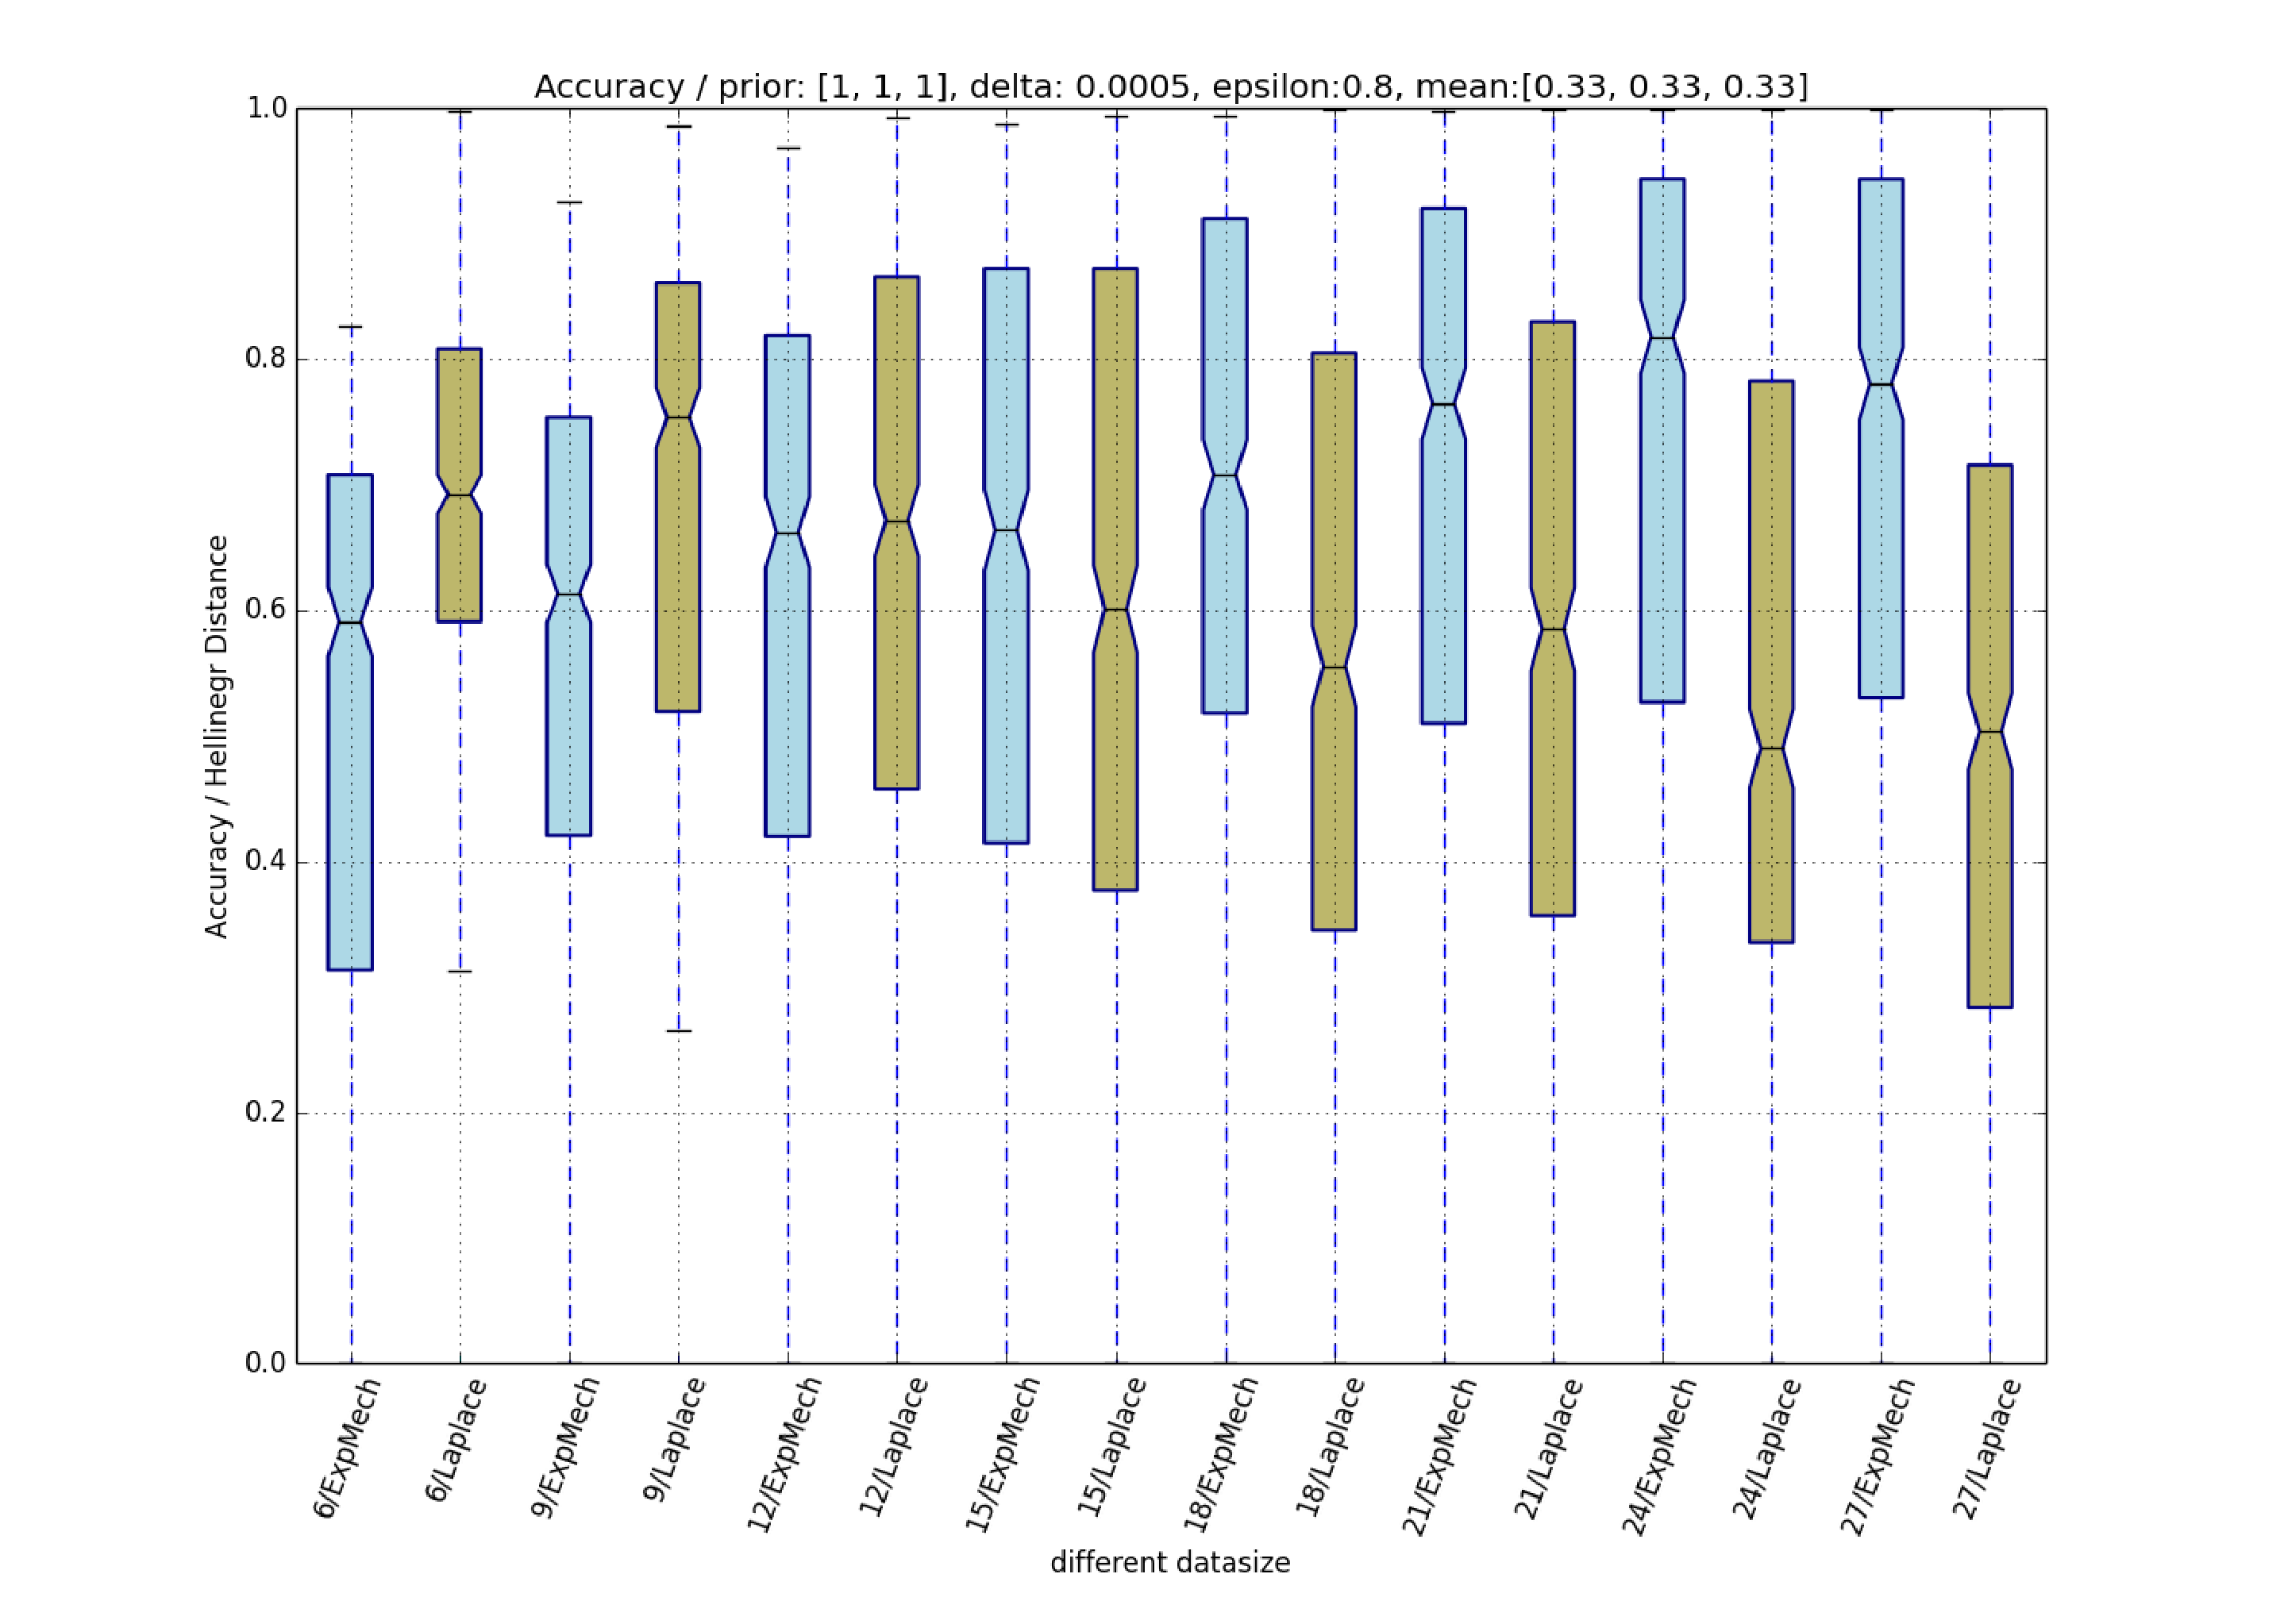
\includegraphics[width=0.3\textwidth]{accuracy_vs_datasize_1_1_1.eps}} 
\caption{Accuracy measurement based on Hellinger distance wrt. different datasizes. Settings: observed data are uniformly distributed, $\epsilon = 0.8$ and $\delta = 0.00000001$}
\label{fig_vs_datasize}
\end{center}
\end{figure}

In Fig. \ref{fig_vs_datasize}, both of the two plots show that when data size go larger, accuracy of our exponential mechanism are decreasing. In Fig. \ref{fig_vs_datasize}(a), when the data size is smaller than 12, we can beta Laplace mechanism but fail when data size larger than or equal to 12. Same as in Fig. \ref{fig_vs_datasize}(b), we can beat Laplace mechanism when data size is smaller than 15 and fail otherwise.

\subsubsection{Accuracy Evaluation wrt. Dimensions}
\label{subsubsec_vs_dimension}


\begin{figure}[ht]
\centering
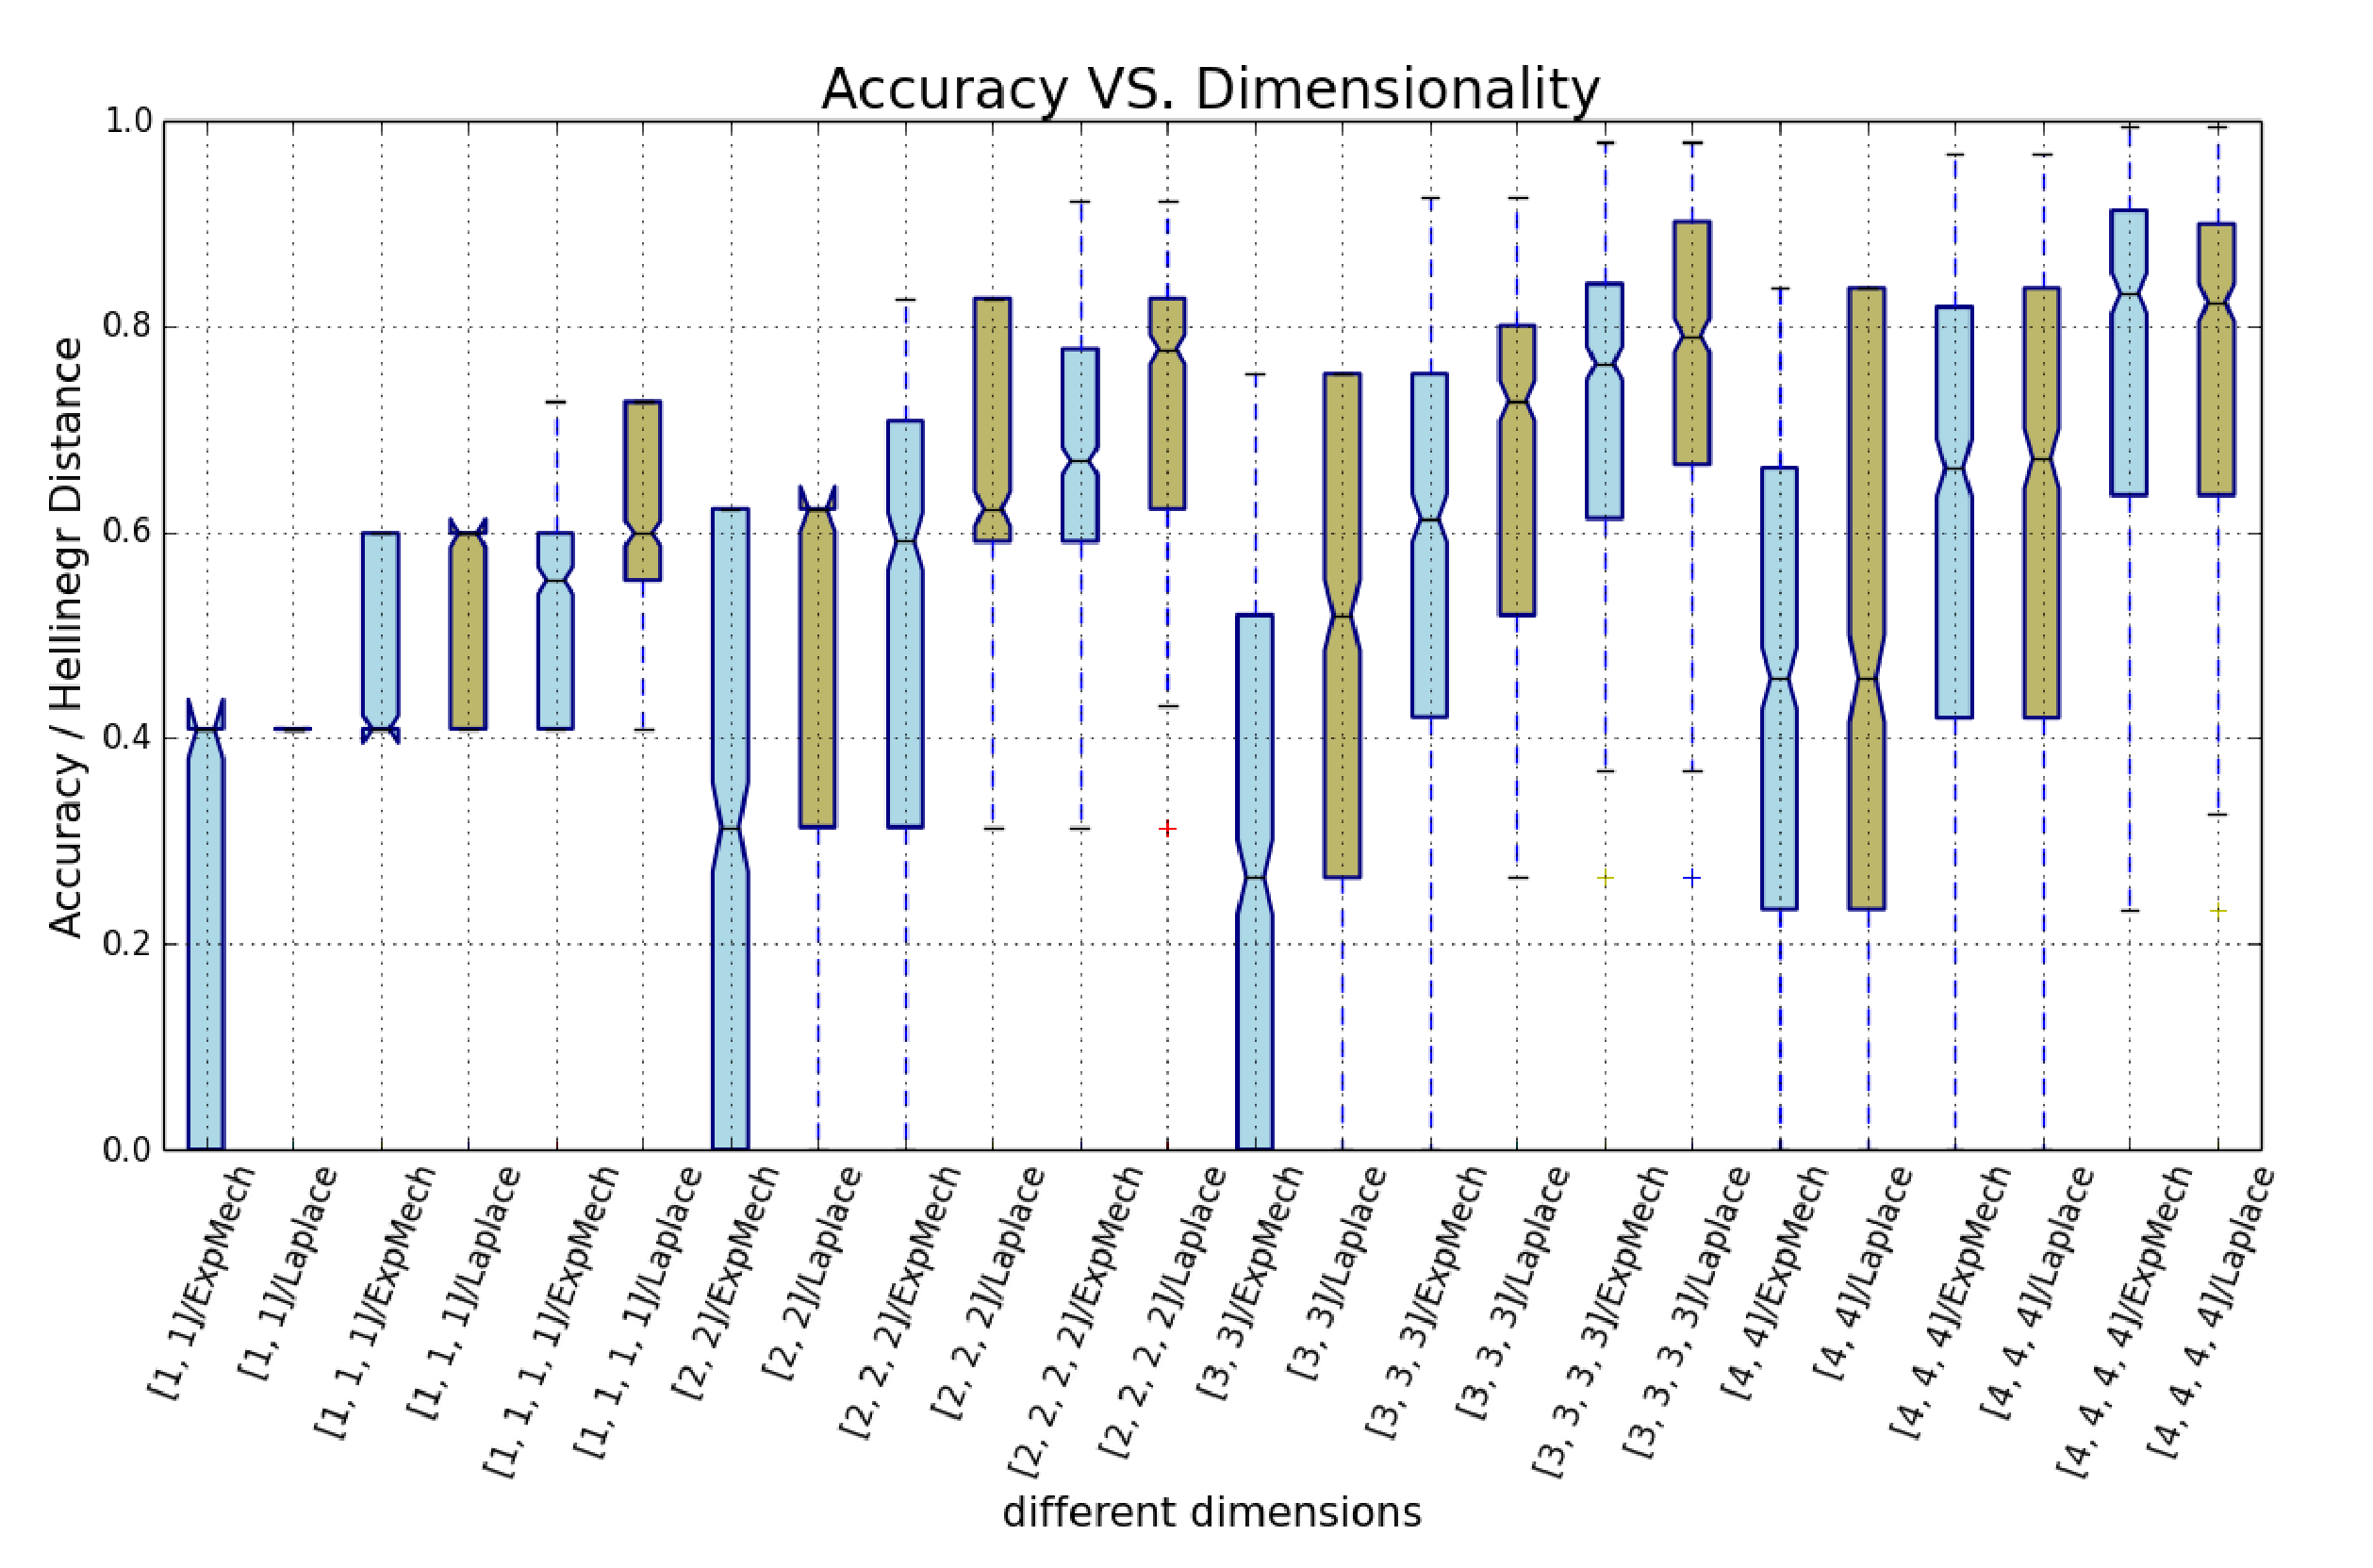
\includegraphics[width=0.45\textwidth]{accuracy_vs_dimension.eps}
\caption{Accuracy measurement based on Hellinger distance wrt. different dimensions and data size. Settings: observed data are uniformly distributed, $\epsilon = 0.8$ and $\delta = 0.00000001$, prior distributions are all $1$ in every dimension}
\label{fig_vs_dimension}
\end{figure}

In Fig. \ref{fig_vs_dimension}, x-axis are observed data sets of different size and dimensions. The plot shows that dimensions have similar influence on our exponential mechanism and the Laplace mechanism. Accuracy of two mechanisms both decrease when dimensions go larger. We will be beat by Laplace mechanism when data size increase but will not be affected when dimensions increase. In other words, dimension has little influence on whether we will beat Laplace mechanism.


\subsubsection{Accuracy Evaluation wrt. Data variance}
\label{subsubsec_vs_variance}

\begin{figure}[ht]
\centering
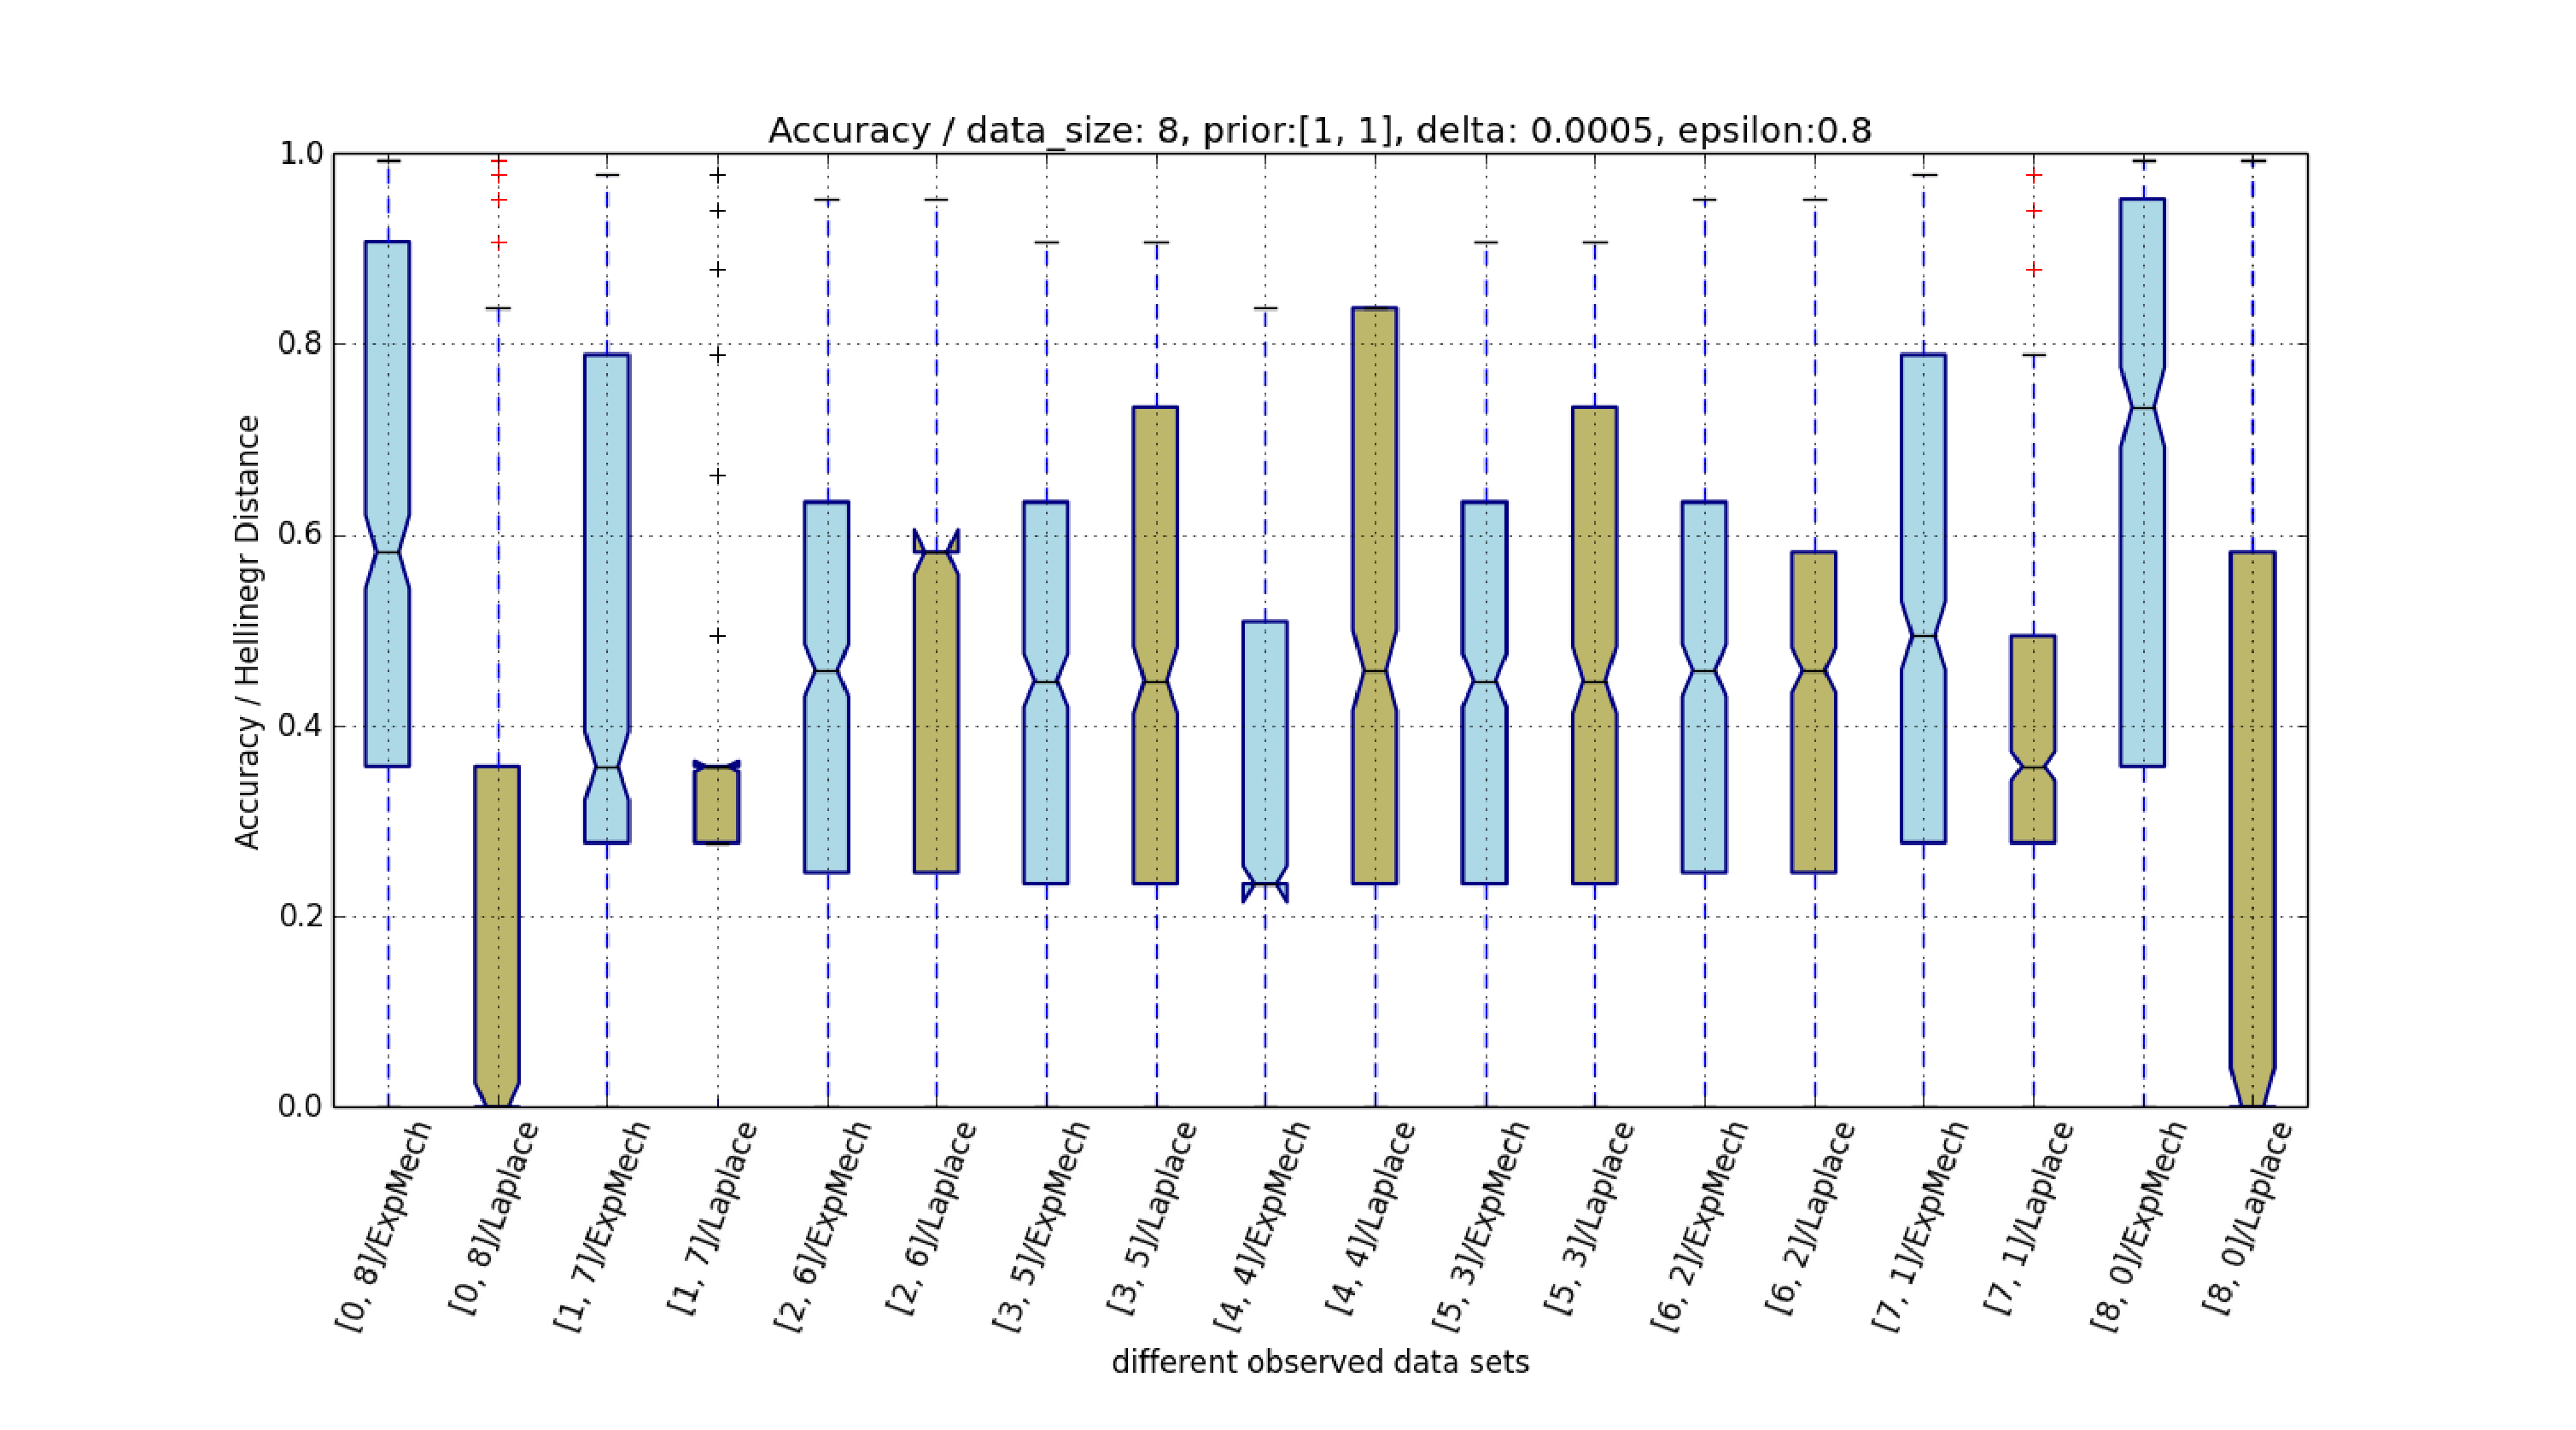
\includegraphics[width=0.45\textwidth]{accuracy_vs_mean_1_1.eps}
\caption{Accuracy measurement based on Hellinger distance wrt. different data variance. Settings: $\epsilon = 0.8$ and $\delta = 0.00000001$, prior distributions are all $1$ in every dimension}
\label{fig_vs_variance}
\end{figure}

In Fig. \ref{fig_vs_variance}, x-axis are observed data sets of different variances (or means). We study this variable under two-dimension $\betad$ distribution in order to be concise. It shows that our mechanism's accuracy is better when data variance go smaller, meanwhile Laplace mechanism go worse. We will beat Laplace mechanism when observed data are more uniformly.



\subsubsection{Accuracy Evaluation wrt. Prior Distribution}
\label{subsubsec_vs_prior}

\begin{figure}[ht]
\centering
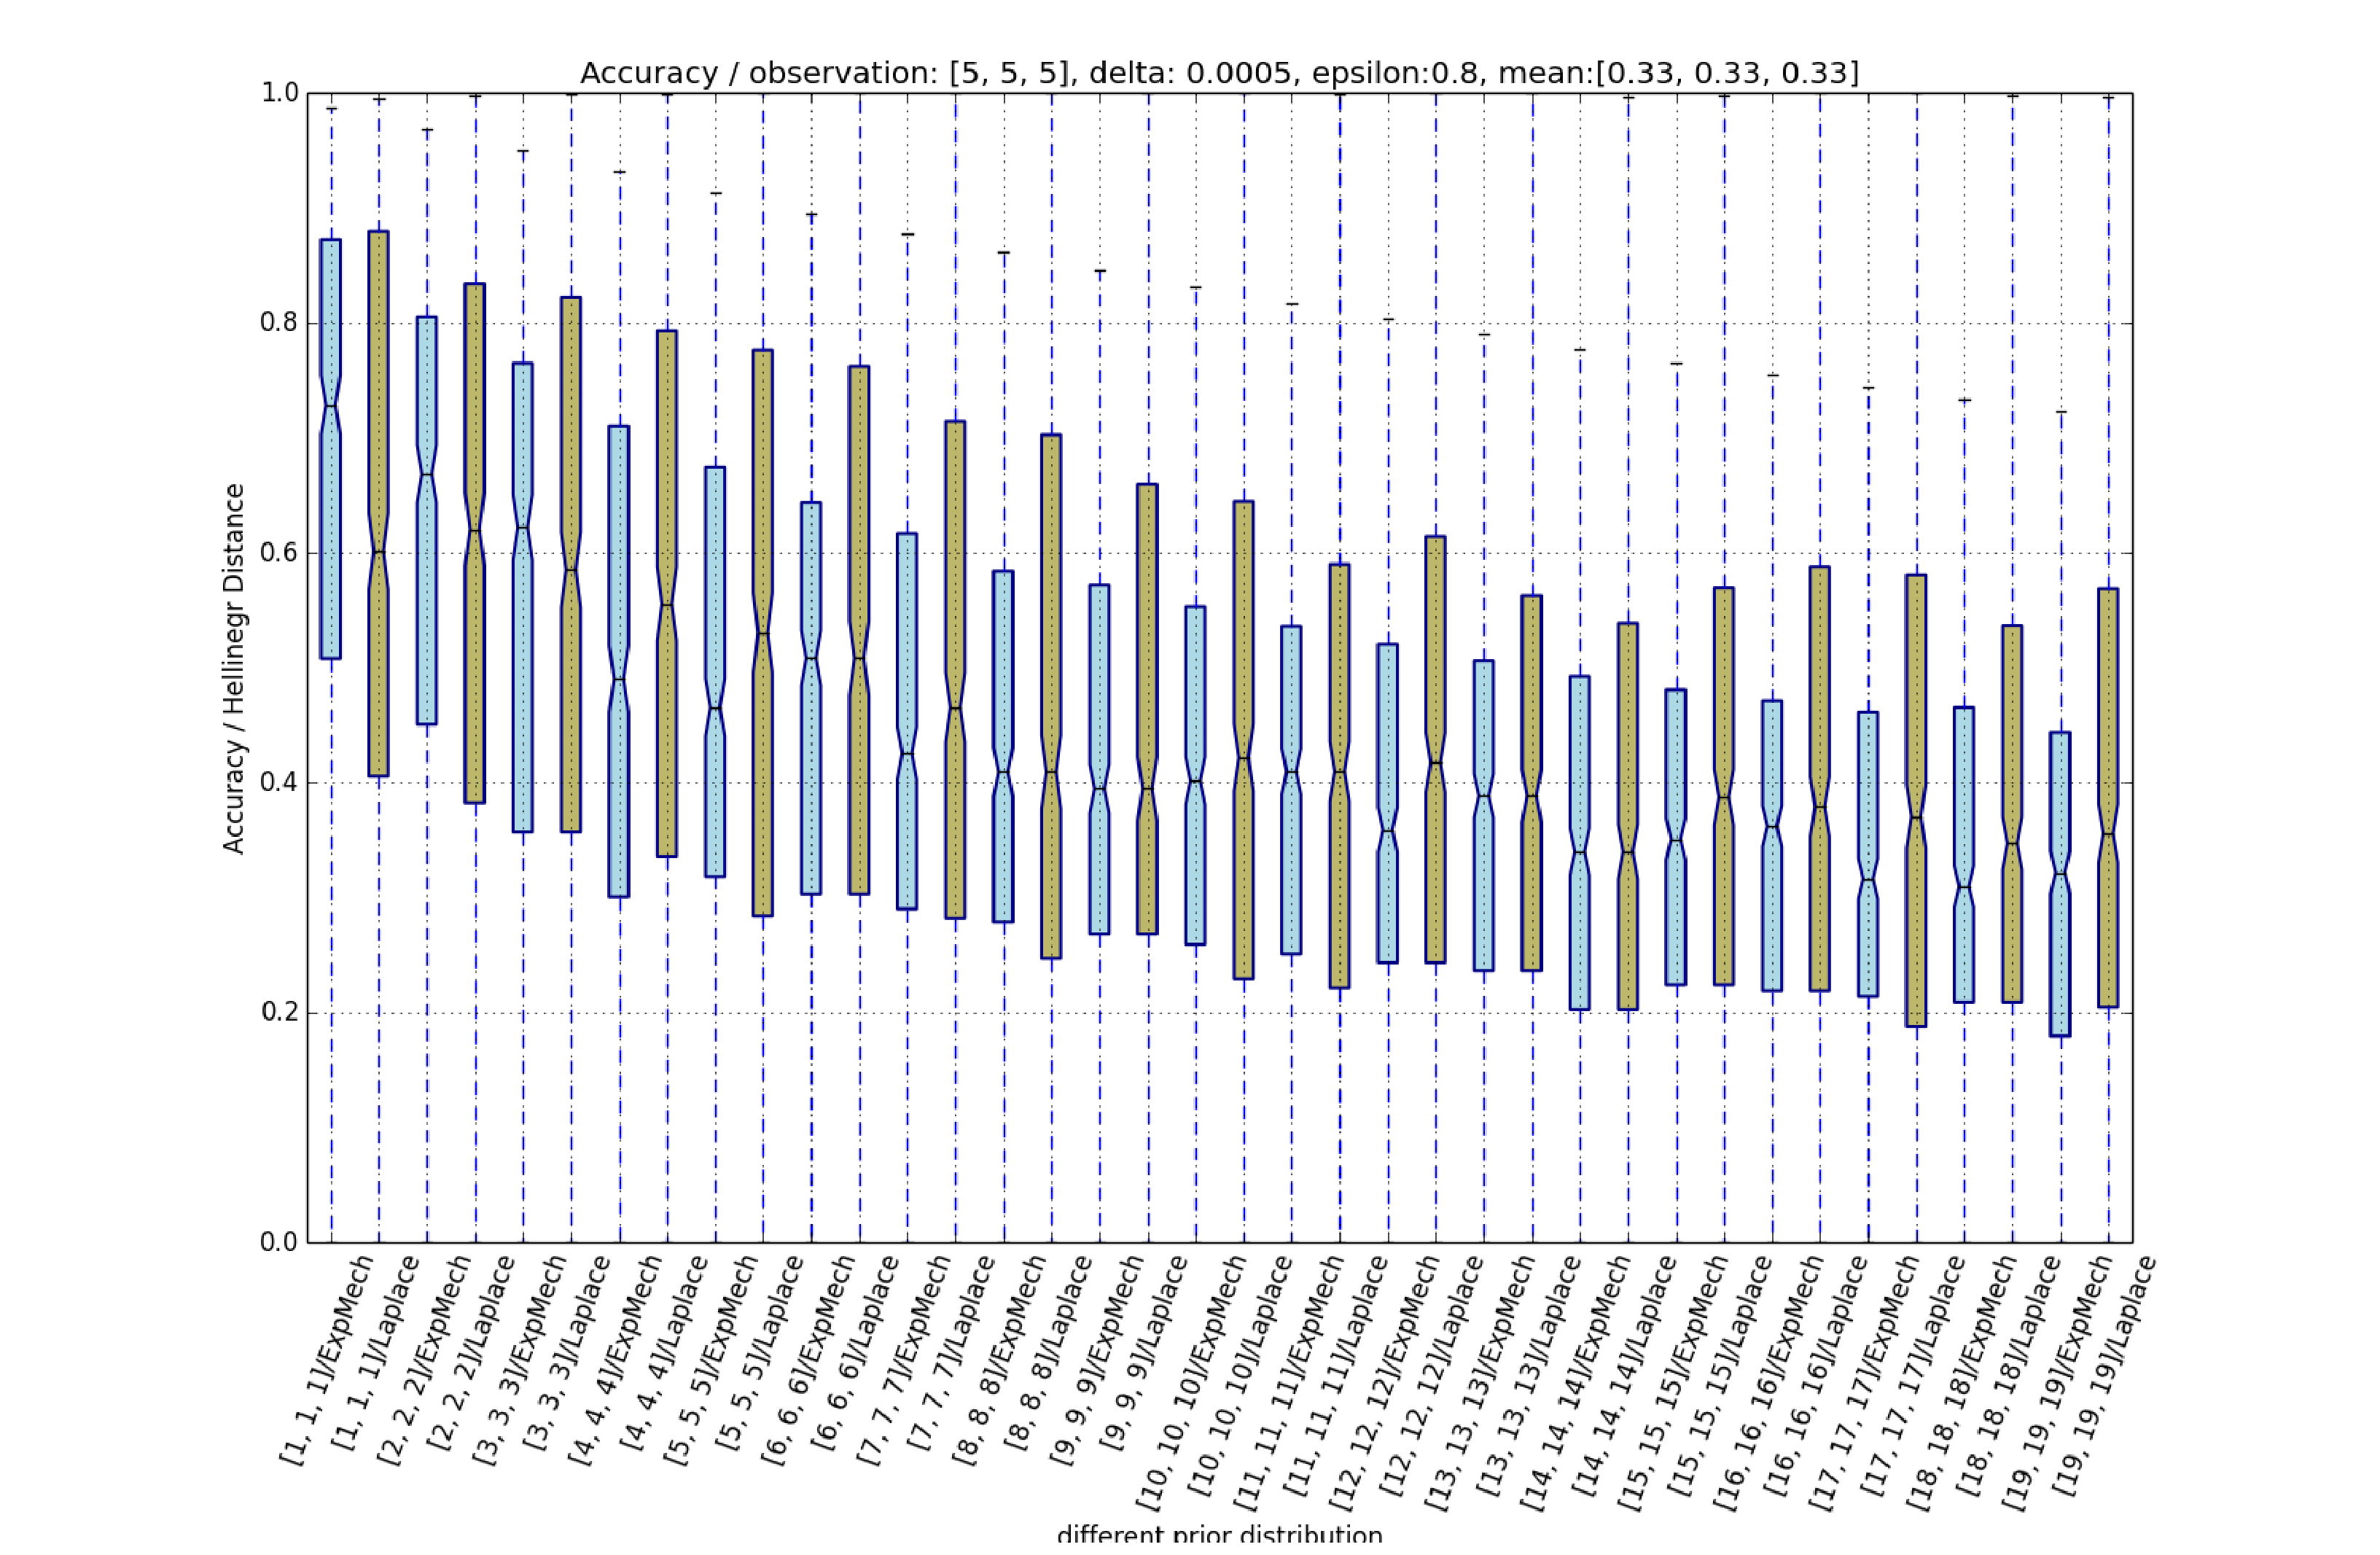
\includegraphics[width=0.45\textwidth]{accuracy_vs_prior_5_5_5.eps}
\caption{Accuracy measurement based on Hellinger distance wrt. different prior distribution. Settings: $\epsilon = 0.8$ and $\delta = 0.00000001$, observed data set is: $[5,5,5]$}
\label{fig_vs_prior}
\end{figure}

In Fig. \ref{fig_vs_prior}, we study this variable under setting that observed data set is $[5,5,5]$ because in Fig. \ref{fig_vs_datasize} Laplace mechanism beat us when data size is 15 and uniformly distributed. The plot shows that in the beginning we cannot beat Laplace but when prior distribution grow larger, we perform better and better and beat Laplace mechanism finally.



% \subsubsection{Accuracy Evaluation wrt. Prior Distribution and Data Variance}
% \label{subsubsec_vs_prior_variance}

% \begin{figure}[ht]
% \centering
% 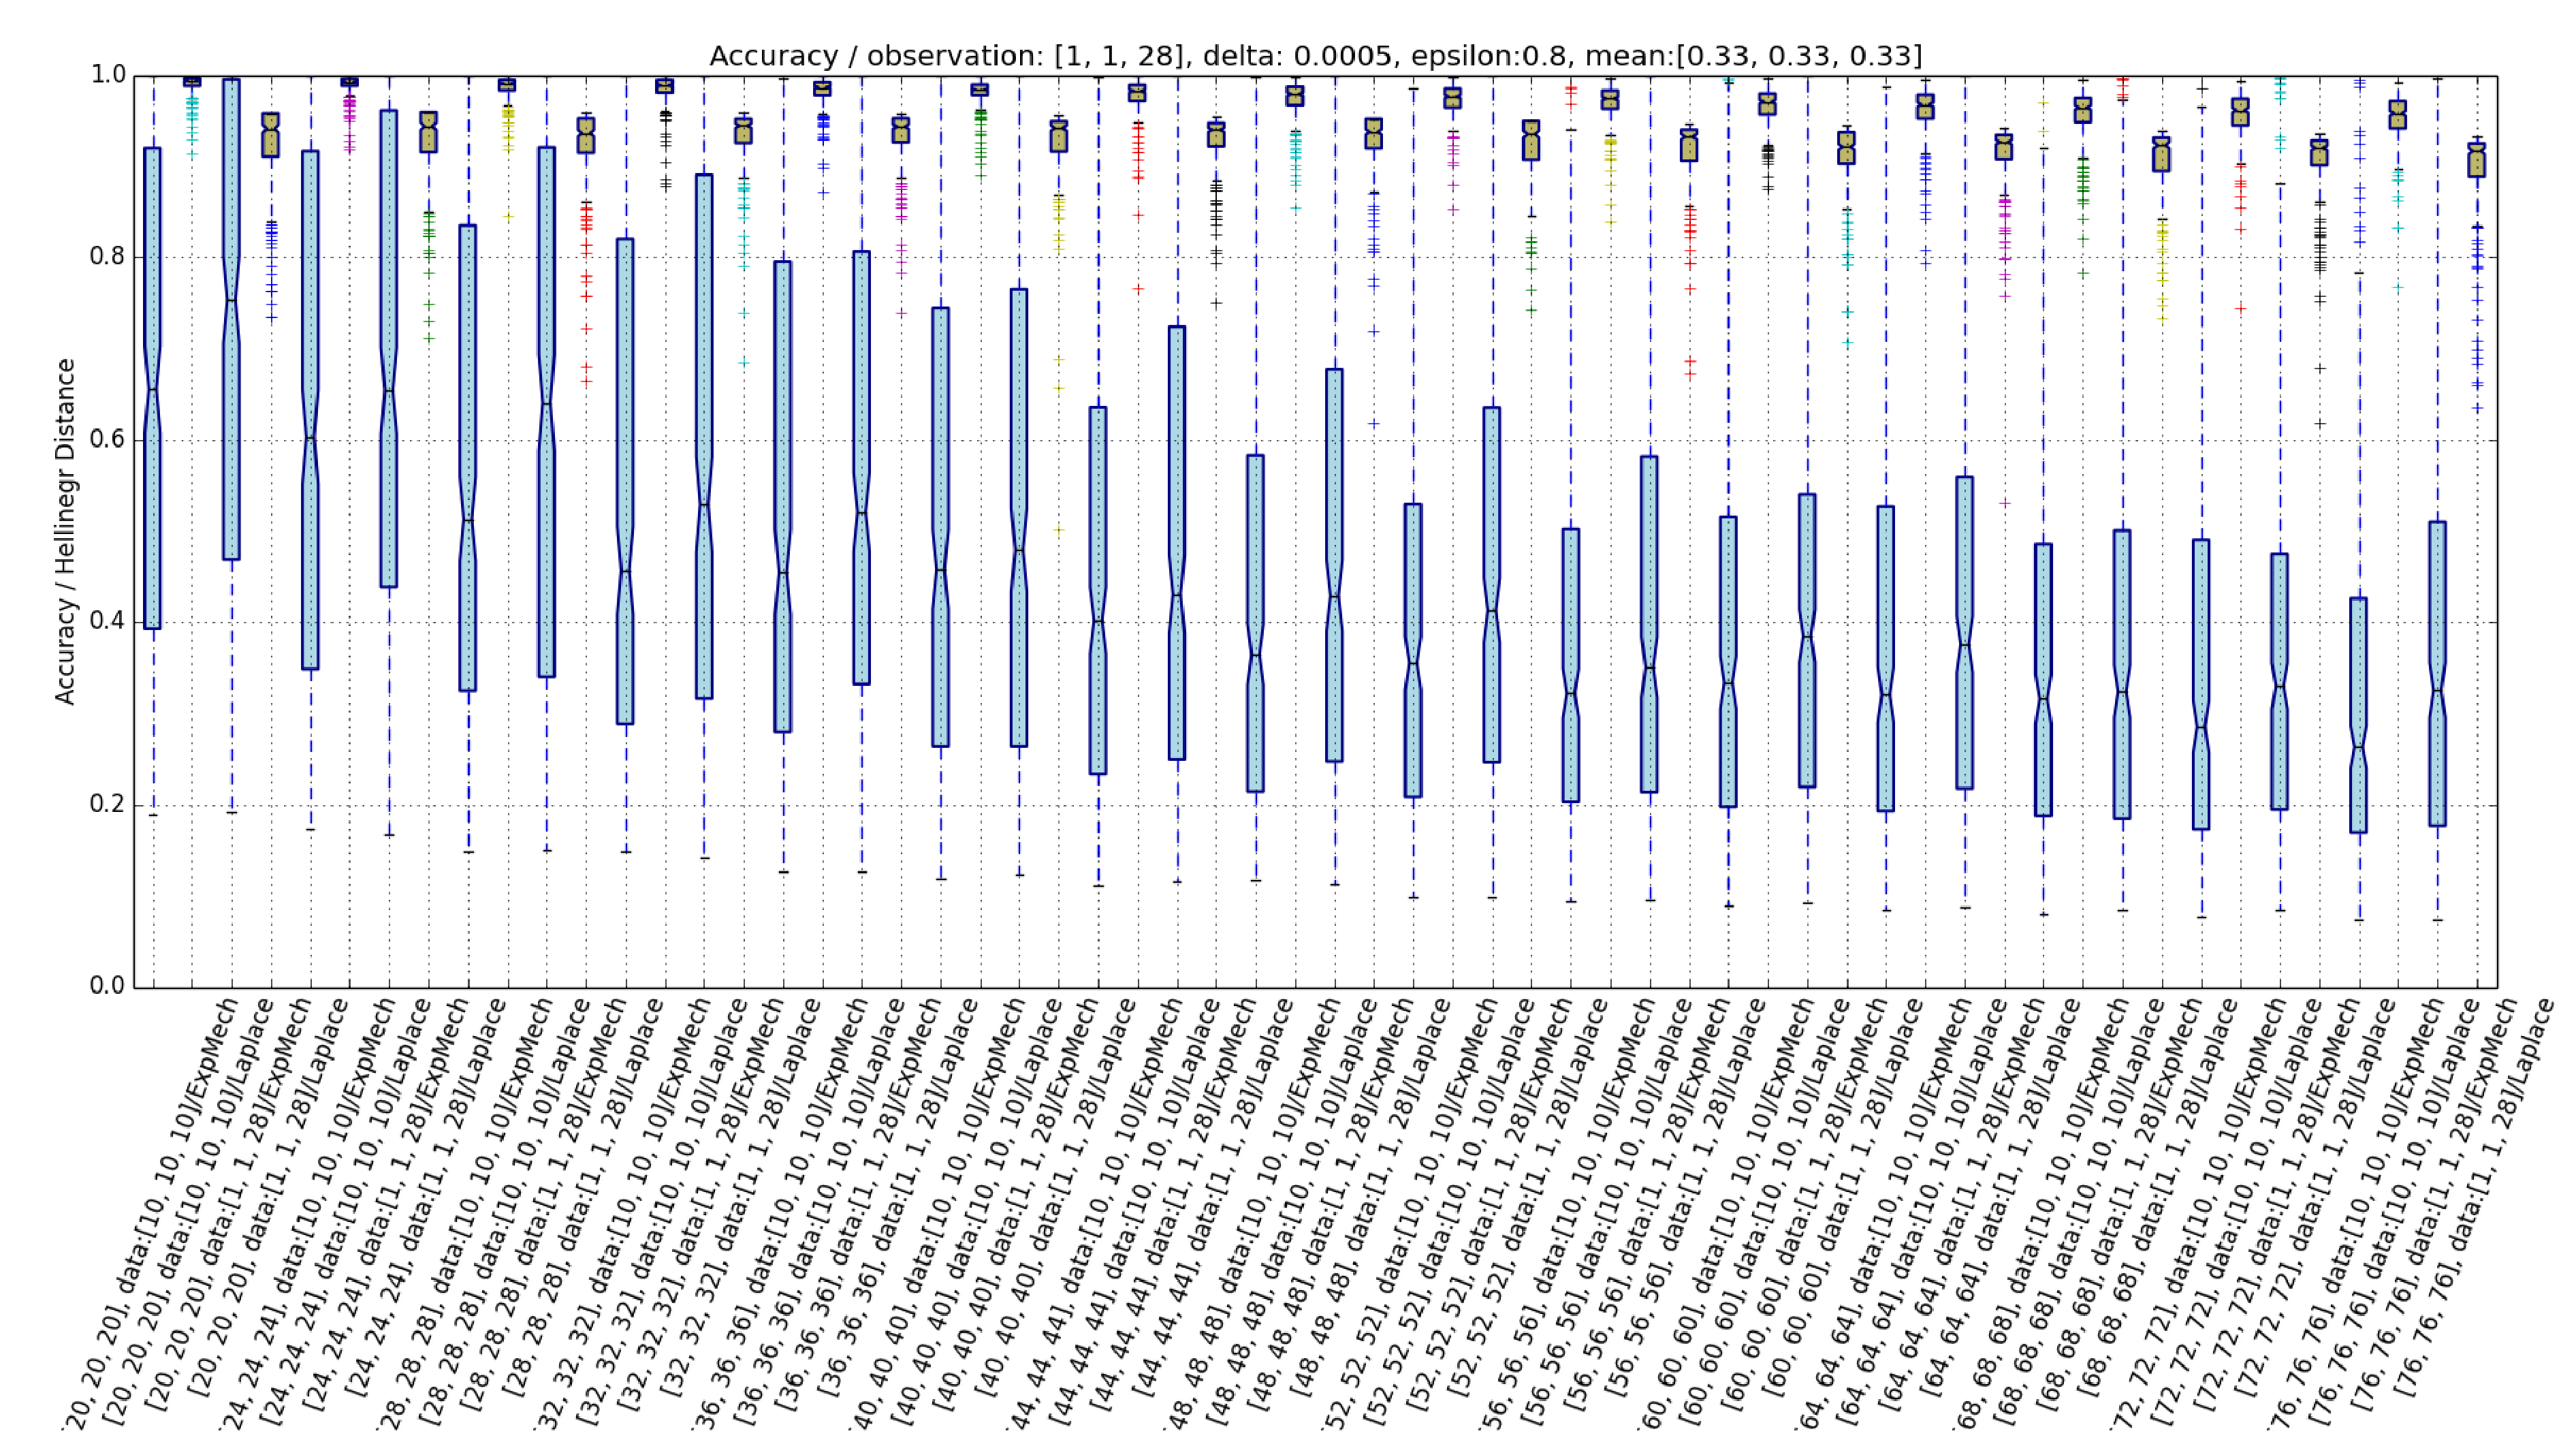
\includegraphics[width=0.45\textwidth]{Accuracy_VS_Prior_mean.eps}
% \caption{Accuracy measurement based on Hellinger distance wrt. different prior distribution and data variances. Settings: $\epsilon = 0.8$ and $\delta = 0.00000001$, observed data sets are $[10,10,10]$ and $[1,1,28]$ and prior distributions are range from $[20,20,20]$ to $[76,76,76]$}
% \label{fig_vs_prior_variance}
% \end{figure}

% Here, we change the prior distribution and data variance in the same time. As shown in Fig. \ref{fig_vs_prior_variance}, our exponential mechanism do better in uniform data set than in edging data set while Laplace mechanism on the contrary. Moreover, our mechanism is improving continuously and significantly as prior distribution increasing while Laplace mechanism isn't.


\section{Conclusions}
We can obtain some preliminary conclusions: 
\begin{enumerate}
	\item We can beat Laplace mechanism when data size is small.
	\item We will beat Laplace mechanism when observed data are more uniformly.
  \item When prior distribution grow larger, we perform better and better and beat Laplace mechanism finally.
\end{enumerate} 

In consequence, we have a better accuracy in small data size, in larger prior and in uniformly data.



\bibliographystyle{ACM-Reference-Format}
\bibliography{bayesian.bib}

\end{document}
